% !TEX TS-program = lualatex
\documentclass[12pt,openany]{book}
%TC:ignore
% This is all the packages and settings and so on.
% It is using custom fonts that needs to be installed on the computer. If they are not present, they have to be added manually.
\usepackage[
	citestyle=ieee, 
    bibstyle=ieee,
    style=numeric-comp,
    sorting=none,
    doi=true, 
    url=true,
    maxbibnames=99, % Make sure we are printing all authors in the appendix
    ]{biblatex}
    
% Makes the last name first in the bibliography.
% \DeclareNameAlias{author}{last-first}
\DeclareNameAlias{author}{family-given}
\AtEveryBibitem{% clear note for bib
  \clearfield{note}%
}

% Specify the margins. This is 6.25inches in text with which 
% can be used to size figures to the correct size.
\usepackage[a4paper, margin=2.5625cm]{geometry}
\usepackage{eso-pic}					% Packages for layout and graphics 
\usepackage{graphicx}
\usepackage{tikz}
\usetikzlibrary{fadings}
\usepackage{setspace}
% \usepackage{tocloft}		 		    % Fixing a bug with page style changes for toc	
% \tocloftpagestyle{plain}
\usepackage{etoc} 						% Separate tocs for appendix and the rest    
\usepackage{chngcntr}					% Count figures within chapters
\usepackage{booktabs}					% Table formatting
\usepackage{fancyhdr}					% Setting the style for header and footer.
\usepackage{tabularx}
\usepackage{multirow}                   % For better tables 
\usepackage[hidelinks]{hyperref}		% Clickable links
\usepackage{nameref}					% References with names
\usepackage[parfill]{parskip}			% New line instead of indent for sections
\usepackage{tcolorbox}					% Create boxes around content
\tcbset{colback=white,arc=0mm}
\usepackage{pgfgantt}                   % For gantt chart 
\usepackage{amsmath}                    % For math
% \usepackage{mathdots}
% \usepackage{yhmath}
\usepackage{siunitx}
% \usepackage{array}
% \usepackage{gensymb}
\usepackage{amssymb}
\usepackage{mathtools}              % Add text to math arrows.
\usepackage{float}
% \usepackage{cancel}
\usepackage{tocloft}                
\usepackage{color}
\usepackage{multirow}
\usepackage{textcomp}               % Fixing warning for gensyb \perthousand
% \usepackage{svg}                    % including svg files
\usepackage{caption}                % For subfigures
\usepackage{subcaption}
% \usepackage{fontspec}
\usepackage{fontawesome}
\usepackage{datetime}
\usepackage{titlesec}               % For title
\usepackage{longtable}              % For long table
% \usepackage{smartdiagram}
\usepackage{overpic}

\usetikzlibrary{chains,shapes.symbols,positioning}
\usepackage[printonlyused]{acronym}

\counterwithin{figure}{section} 
\counterwithin{table}{section}

% Specifying fonts
\setmainfont{TeX Gyre Termes} 
% \setmainfont{Georgia} 
\setsansfont{Arial}
\newfontfamily\footerfont{Georgia}

% \chapterfont{\sffamily\fontsize{17}{17}}
% \sectionfont{\sffamily\fontsize{14}{15}}
% \subsectionfont{\sffamily\fontsize{13}{15}}
% \subsubsectionfont{\sffamily\fontsize{12}{15}}
% \titleformat{\chapter}[display]
%   {\normalfont\sffamily\huge\bfseries}
%   {\chaptertitlename \thechapter}{17pt}{\Huge}
% \titleformat{\section}
%   {\normalfont\sffamily\Large\bfseries}
%   {\thesection}{1em}{}

% Remove the title and make sure that the text is adjusted
% \usepackage{abstract}
% \setlength{\absleftindent}{0mm}
% \renewcommand{\abstractname}{\vspace{-\baselineskip}}
% \renewcommand{\abstractnamefont}{\sffamily\fontsize{14}{15}}
% \renewcommand{\abstracttextfont}{\normalfont\fontsize{12}{13}}

% Renaming and setting style of table of contents
\renewcommand*\contentsname{Contents}
\renewcommand*\cfttoctitlefont{\fontsize{16}{0}\bf\sffamily}
\renewcommand\cftchapfont{\fontsize{14}{0}\bf\sffamily}
\renewcommand\cftchappagefont{\fontsize{13}{0}\bf\sffamily}
\renewcommand\cftsecfont{\fontsize{12}{0}\sffamily}
\renewcommand\cftsecpagefont{\fontsize{12}{0}\sffamily}
\renewcommand\cftsubsecfont{\fontsize{12}{0}\sffamily}
\renewcommand\cftsubsecpagefont{\fontsize{12}{0}\sffamily}

% Styling the header and footer
\fancyhf{}
\fancyhead{}
\fancyfoot{}
\fancyhead[OL]{\selectfont\leftmark}
\fancyhead[OR]{\selectfont\thepage}
\fancyhead[ER]{\selectfont\rightmark}
\fancyhead[EL]{\selectfont\thepage}
% \fancyfoot[R]{\footerfont\thepage}
\setlength{\headheight}{15.5pt}

\fancypagestyle{plain}{
    \fancyhf{}
    % \fancyheadoffset{1cm}
    \setlength{\headheight}{0em}
    
    % \fancyhead{}
    % \fancyfoot{}
    \renewcommand{\headrulewidth}{0pt}
    \fancyfoot[C]{\footerfont\thepage}
}

\titlespacing*{\chapter}{0pt}{0pt}{10pt}
\AtBeginDocument{\addtocontents{toc}{\protect\thispagestyle{empty}}}
\pagestyle{fancy}

% Making the command for placing text in random locations
\newcommand\PlaceText[3]{%
\begin{tikzpicture}[remember picture,overlay]
\node[outer sep=0pt,inner sep=0pt,anchor=south west] 
  at ([xshift=#1,yshift=-#2]current page.north west) {#3};
\end{tikzpicture}%
}

% Disable hyphenation
\pretolerance=10000
\tolerance=2000 
\emergencystretch=50pt

% \AtBeginBibliography{\small}

% Defining files for bibliography
\addbibresource{references.bib}
% Add a second bibliography file for the second author to allow
% both to update it through the mendeley integration.
% \addbibresource{ref-author-2.bib}

% Defining document information
\title{Optimal Gait Control of Soft Quadruped Robot by Model-based Reinforcement Learning}

\author{NIU Xuezhi}

\begin{document}
\setstretch{1.25}

% The front page of the document
\pagenumbering{Roman}
\makeatletter
\begin{titlepage}

\vspace*{-4.6\baselineskip}
\hspace*{-0.15\textwidth}
\includegraphics[width=0.2\paperwidth]{setup/img/kth-logo.jpg}
\par\vspace*{2.5\baselineskip}

\PlaceText{65mm}{12mm}{\fontsize{12}{0}\sffamily DEGREE PROJECT IN MECHATRONICS,}
\PlaceText{65mm}{17mm}{\fontsize{12}{0}\sffamily SECOND CYCLE, 30 CREDITS}
\PlaceText{65mm}{22mm}{\fontsize{12}{0}\sffamily\itshape STOCKHOLM, SWEDEN \the\year}
~\\

\makebox[0pt][l]{%
\begin{minipage}[b]{0.25\textwidth}
~\\
\end{minipage}
\begin{minipage}{0.65\textwidth}
\begin{flushleft}
{\fontsize{25}{20}\bf\sffamily\@title\\}
\vspace{1cm}
% {\fontsize{19}{17}\bf\sffamily \subtitle\\}
% \vspace{1cm} 
{\fontsize{20}{18}\sffamily \@author}\\
\end{flushleft}
\end{minipage}
}


% \hspace*{-3cm}\begin{minipage}[b]{63.5mm}
% ~\\
% \end{minipage}
% \begin{minipage}{0.65\textwidth}
% \begin{flushleft}
% {\fontsize{28}{24}\bf\sffamily\@title\\}
% \vspace{0.5cm}
% {\fontsize{19}{17}\bf\sffamily \subtitle\\}
% \vspace{0.5cm} 
% {\fontsize{16}{0}\sffamily \@author}\\
% \end{flushleft}
% \end{minipage}


\AddToShipoutPictureBG*{%]
    \AtPageLowerLeft{%
        
\includegraphics[width=1.0\paperwidth]{setup/img/kth-footer.png}
    }%
}

\PlaceText{70mm}{280mm}{\color{white}\fontsize{12}{0}\sffamily KTH ROYAL INSTITUTE OF TECHNOLOGY }
\PlaceText{70mm}{285mm}{\color{white}\fontsize{10}{0}\sffamily SCHOOL OF INDUSTRIAL ENGINEERING AND MANAGEMENT}
\end{titlepage}
\makeatother

\newpage
\pagestyle{myempty}
\newpage
\thispagestyle{empty}
~\\
\vfill
{ \setstretch{1.1}
	\subsection*{Authors}
	NIU Xuezhi { }$\langle$\href{mailto:xuezhin@kth.se}{xuezhin@kth.se}$\rangle$\\
    Msc. in Engineering Design - Mechtronics \\
	KTH Royal Institute of Technology
	
	\subsection*{Place for Project}
	Stockholm, Sweden
	
	\subsection*{Examiner}
	Lei Feng \\
	Department of Machine Design \\
	KTH Royal Institute of Technology
	
	\subsection*{Supervisor }
	Tan Kaige\\
 % Mechatronics and Embedded Control Systems division, 
    Department of Machine Design\\
	KTH Royal Institute of Technology
	~
}

\titleformat
{\chapter} % command
[display] % shape
{\normalfont\huge\bfseries} % format
{\hfill \thechapter} % label
{-2ex} % sep
{
    \vspace{-1.2em}
    \begin{table}[hp]
    \centering
    {\sffamily
    \resizebox{\textwidth}{!}{%
    \begin{tabular}{|cp{5cm}p{5cm}|}
        \hline
        \multicolumn{1}{|p{3.875cm}}{\begin{tabular}[l]{@{}c@{}}\includegraphics[width=0.5\linewidth]{setup/img/kth\_logo.eps}\\ \tiny\sffamily\bfseries KTH Industriell Teknik \vspace*{-0.3cm}\\ \tiny\sffamily\bfseries och Management\end{tabular}} &
          \multicolumn{2}{c|}{\begin{tabular}[c]{@{}c@{}}\textbf{Examensarbete TRITA-ITM-EX 2023:XXX}\\ \\ \\ \textbf{Adaptiv gångstyrning av en mjuk fyrbent robot} \\ \textbf{genom modellbaserad förstärkningsinlärning}\vspace{2em}\end{tabular}} \\
        \multicolumn{1}{|c}{} &
          \multicolumn{2}{c|}{NIU Xuezhi} \\ \hline
        \multicolumn{1}{|l|}{\begin{tabular}[c]{@{}l@{}}\scriptsize Godkänt\\ \normalsize 2023-mån-dag\end{tabular}} &
          \multicolumn{1}{p{5cm}|}{\begin{tabular}[c]{@{}l@{}}\scriptsize Examinator\\ \normalsize Lei Feng\end{tabular}} &
          \begin{tabular}[c]{@{}l@{}}\scriptsize Handledare\\ \normalsize Tan Kaige\end{tabular} \\ \hline
        \multicolumn{1}{|p{5cm}|}{} &
          \multicolumn{1}{l|}{\begin{tabular}[c]{@{}l@{}}\scriptsize Uppdragsgivare\\ \normalsize Lei Feng\end{tabular}} &
          \begin{tabular}[c]{@{}l@{}}\scriptsize Kontaktperson\\ \normalsize Lei Feng\end{tabular} \\ \hline
    \end{tabular}%
    }}
\end{table}

    \vspace{-1em}
    % \noindent
    \makebox[0pt][l]{\rule[.6ex]{\linewidth}{2.5pt}}%
    \rule[.3ex]{\linewidth}{.6pt}
    % \vspace{-0.5ex}
} % before-code
[
\vspace{-2ex}%
\rule{\textwidth}{.6pt}
] % after-code

\newpage
%%%%%%%%%%%%%%%%%%%%%%%%%%%%%%%%%%%%
%%	 The Swedish abstract         %%
%%%%%%%%%%%%%%%%%%%%%%%%%%%%%%%%%%%%
\chapter*{Sammanfattning}
%%%%%%%%%%%%%%%%%%%%%%%%%%%%%%%%%%%%

Fyrbenta robotar har fördelen att kunna manövrera i komplex terräng utan mänsklig ansträngning, och de kan till exempel ge större absorptionsförmåga så att roboten bättre kan stå emot stötar och slag. Även om stela robotar är kända för sin snabba respons och exakta rörelser, kan de vara begränsade i sitt rörelseområde på grund av sina stela mekaniska strukturer, såsom leder och hydrauliska ställdon. På senare tid har utvecklingen av sensorer, ställdon och datorer gjort det lättare att styra mjuka fyrbenta robotar i verkliga livet, vilket gör det möjligt att utforska styrstrategier för ökad anpassningsförmåga och effektivitet i olika terränger och miljöer. Samtidigt underlättar användningen av förstärkningsinlärning för styrning av robotteknik uppnåendet av autonoma och anpassningsbara robotbeteenden, där robotar lär sig att agera genom interaktioner med sina miljöer för att optimera prestanda. 

Trots framstegen inom styrning av fyrbenta robotar kräver integrering av avancerade styrmetoder som förstärkningsinlärning omfattande utbildning och robusthetsöverväganden för att säkerställa säker funktionalitet i den verkliga världen. Att anpassa effektiva simuleringsbaserade styrtekniker till konkreta robotar stöter på utmaningar som härrör från skillnaden mellan simulerade och verkliga miljöer, vilket kräver förbättrade metoder för förstärkningsinlärning. Denna avhandling strävar efter att bidra väsentligt till att öka robotförmågan genom att använda en optimal gångkontroll av mjuka fyrhjuliga robotar genom modellbaserad förstärkningsinlärning. Genom att ta itu med de utmaningar som är kopplade till den verkliga implementeringskomplexiteten och förfina kontrollstrukturerna, syftar den till att bana en transformativ väg för en harmonisk sammanslagning av förstärkningsinlärning i den mjuka fyrhjuliga robotdomänen, vilket förbättrar prestanda, anpassningsförmåga och autonomi.

Inom innehållet i denna rapport ingår implementeringen av modellbaserade tekniker för förstärkt inlärning för att optimera gångkontrollen, med detaljer om simuleringsinställningen, belöningsstrukturen och policyförfiningsprocessen. En omfattande presentation av resultaten tillhandahålls, tillsammans med en djupgående analys som validerar effektiviteten hos de föreslagna metoderna. Analysen visar på betydande förbättringar av träningseffektiviteten och det autonoma beteendet, vilket i slutändan bekräftar effektiviteten hos de föreslagna metoderna. 

\subsection*{Nyckelord}
Fyrhjuliga robotar, mjuk robotteknik, adaptiv gångkontroll, modellbaserad förstärkningsinlärning


% \pagestyle{plain}
\titleformat
{\chapter} % command
[display] % shape
{\normalfont\huge\bfseries} % format
{\hfill \thechapter} % label
{-2ex} % sep
{
    \vspace{-1.2em}
    \selectfont
\begin{table}[hp]
    \centering
    {\sffamily
    \resizebox{\textwidth}{!}{%
    \begin{tabular}{|cp{5cm}p{5cm}|}
        \hline
        \multicolumn{1}{|p{3.875cm}}{\begin{tabular}[l]{@{}c@{}}\includegraphics[width=0.5\linewidth]{setup/img/kth\_logo.eps}\\ \tiny\bfseries KTH Industrial Engineering \vspace*{-0.3cm}\\ \tiny\bfseries and Management\end{tabular}} &
          \multicolumn{2}{c|}{\begin{tabular}[c]{@{}c@{}}\textbf{Master of Science Thesis TRITA-ITM-EX 2023:XXX}\\ \\ \\ \textbf{Adaptive Gait Control of Soft Quadruped Robot} \\ \textbf{by Model-based Reinforcement Learning}\vspace{2em}\end{tabular}} \\
        \multicolumn{1}{|c}{} &
          \multicolumn{2}{c|}{NIU Xuezhi} \\ \hline
        \multicolumn{1}{|l|}{\begin{tabular}[c]{@{}l@{}}\scriptsize Approved\\ \normalsize 2023-month-day\end{tabular}} &
          \multicolumn{1}{p{5cm}|}{\begin{tabular}[c]{@{}l@{}}\scriptsize Examiner\\ \normalsize Lei Feng\end{tabular}} &
          \begin{tabular}[c]{@{}l@{}}\scriptsize Supervisor\\ \normalsize Tan Kaige\end{tabular} \\ \hline
        \multicolumn{1}{|p{5cm}|}{} &
          \multicolumn{1}{l|}{\begin{tabular}[c]{@{}l@{}}\scriptsize Commissioner\\ \normalsize Lei Feng\end{tabular}} &
          \begin{tabular}[c]{@{}l@{}}\scriptsize Contact person\\ \normalsize Lei Feng\end{tabular} \\ \hline
    \end{tabular}%
    }}
\end{table}

    \vspace{-1em}
    % \noindent
    \makebox[0pt][l]{\rule[.6ex]{\linewidth}{2.5pt}}%
    \rule[.3ex]{\linewidth}{.6pt}
    % \vspace{-0.5ex}
} % before-code
[
\vspace{-2ex}%
\rule{\textwidth}{.6pt}
] % after-code

\newpage
\pagenumbering{Roman}
% \thispagestyle{plain}
%%%%%%%%%%%%%%%%%%%%%%%%%%%%%%%%%%%%
%%  The English abstract          %%
%%%%%%%%%%%%%%%%%%%%%%%%%%%%%%%%%%%%
\chapter*{Abstract}
%%%%%%%%%%%%%%%%%%%%%%%%%%%%%%%%%%%%

Quadruped robots share advantages of maneuverability in complex terrain without human effort; for instance, they can provide greater absorption capacity, allowing the robot to withstand impacts and shocks better. While rigid robots are known for their fast response and motion accuracy, they may be limited in their motion range due to their rigid mechanical structures, such as joints and hydraulic actuators. Recently, the advancement in sensors, actuators, and computers have facilitated the easy real-life control of soft quadruped robots, enabling the exploration of control strategies for enhanced adaptability and efficiency in diverse terrains and environments. Meanwhile, the utilization of reinforcement learning for the control of robotics facilitates the attainment of autonomous and adaptable robotic behaviors, where robots learn to act through interactions with their environments to optimize performance. 

Nevertheless, despite progress in control of quadruped robotics, integrating advanced control methods like reinforcement learning necessitates extensive training and robustness considerations for ensuring secure real-world functionality. Adapting effective simulation-based control techniques to tangible robots encounters challenges stemming from the disparity between simulated and real-world environments, demanding improved reinforcement learning methodologies. This thesis strikes to contribute significantly to the augmentation of robotic capabilities by employing an optimal gait control of soft quadruped robots through model-based reinforcement learning. By addressing the challenges tied to real-world implementation complexities and refining control structures, it aims to pave a transformative pathway for the harmonious amalgamation of reinforcement learning into the soft quadruped robotics domain, enhancing performance, adaptability, and autonomy.

Within the contents of this report, the implementation of model-based reinforcement learning techniques to optimize gait control is included, detailing the simulation setup, reward structure, and policy refinement process. A comprehensive presentation of the results is provided, along with an in-depth analysis that validates the effectiveness of the proposed methodologies. This analysis reveals notable improvements in training efficiency and autonomous behavior, ultimately affirming the efficacy of the undertaken methods.

\vspace{2cm}
\subsection*{Keywords:}
Quadruped Robots, Soft Robotics, Optimal Gait Control, Model-Based Reinforcement Learning(MBRL)


\titleformat
{\chapter} % command
[display] % shape
{\normalfont\huge\bfseries} % format
{\hfill Chapter \ \thechapter} % label
{-2ex} % sep
{
    % \noindent
    \makebox[0pt][l]{\rule[.6ex]{\linewidth}{2.5pt}}%
    \rule[.3ex]{\linewidth}{.6pt}
    % \vspace{-0.5ex}
} % before-code
[
\vspace{-2ex}%
\rule{\textwidth}{.6pt}
] % after-code

\newpage
\chapter*{Acknowledgements}
I am deeply grateful for the opportunity to complete this Master's Thesis and would like to acknowledge the support and guidance of several individuals who have contributed to the successful completion of this project.

First and foremost, I would like to extend my sincere thanks to the Mechatronics Department of Machine Design at KTH for their unwavering support throughout the duration of this project. I am particularly indebted to my academic supervisor, Mr. Tan Kaige, for his guidance and unwavering commitment to keeping me on track. Moreover, I would like to express my deep appreciation to the examiner, Prof. Lei Feng, for his interest in my work and for his valuable consultation. Dr. Fredrik Asplund deserves my gratitude for his invaluable guidance and advice regarding the research methodology, which helped shape the initial direction of this thesis work. In addition, I appreciate the assistance of Seshagopalan Thorapalli Muralidharan in identifying and resolving potential issues related to the electrical board and wiring. 

I cannot overlook the unwavering support of my parents throughout my academic journey, and I deeply appreciate their encouragement, which has been a constant source of motivation. Furthermore, I would like to recognize the contribution of ChatGPT, the language model developed by OpenAI, for its assistance in refining some certain written content included in this thesis.

Lastly, I would also like to acknowledge myself, as I am also proud of the dedication, perseverance, and hard work I have put into completing this Master's Thesis.

\vspace{2cm}
\hfill NIU Xuezhi 牛雪芝

\hfill Stockholm, \monthname{ }2023 $\ddot\smile$

\newpage

\chapter*{Acronyms}

\section*{Abbreviations}
\begin{acronym}[RDBMS]
\acro{3D}{Three Dimensional}
\acro{4D}{Four Dimensional}
\acro{DoF}{Degree of Freedom}
\acro{RL}{Reinforement Learning}
\acro{MBRL}{Model-Based Reinforement Learning}
\acro{MFRL}{Model-Free Reinforement Learning}
\end{acronym}

\section*{General mathematics}




\newpage

\etocdepthtag.toc{mtchapter}
\etocsettagdepth{mtchapter}{subsection}
\etocsettagdepth{mtappendix}{none}

\tableofcontents
\newpage
%TC:endignore
\setstretch{1.25}
\pagestyle{myfancy}
\section{Requirements}
Abstract and Introduction: Concise overview of the research field relevant to the Master’s thesis, and identification of important open questions. Clear description of the problem addressed in the thesis, and clear statement of the project goals. Appropriate literature citations in a uniform and consistent style and format (applies to whole thesis)

Methods and Results: Clear and complete description of the methods used such that all experiments can be reproduced by others. Clear description of the logic and hypotheses underlying the choice of performed experiments. Clear and complete presentation and correct interpretation of the experimental results. Appropriate quality and quantity of results. Correct presentation and labelling of figures and tables.

Discussion and Conclusions: Concise discussion and critical evaluation of the obtained results with respect to the original goals. Discussion of the results into a more general context within the research field. Discussion of the possibilities and limitations of the applied experimental techniques. Formulation of new hypotheses, outlook for future work.
A) Abstract
An abstract that allows an "informed reader" to grasp the contents of the report. This abstract should be 100% finished at the 80%-draft of the report.
B) Introduction
Define the background of your project, the purpose of the report, specific descriptions of problems, your research questions, any limitations to the scope of your investigation, and (briefly) your chosen methodology.
C) Related Work / Theoretical Background / Theoretical Framework
It is necessary to describe the relevant, scientific background knowledge concerning the area in which you will perform your thesis work. One goal of this section is to analyse the literature reviewed and thus specify the direction of your project work. The main goal is for you to build on and expand your existing knowledge to assist you in dealing with the task at hand. This section is ideally structured as describing related work (scientific papers that perform variants of the same investigation as you do), as a theoretical background (scientific papers that deal with the same problem area as you do), or as a theoretical framework (scientific papers that you use to create a theoretical model for explaining your results).
D) Methodology
Describe the scientific methodology that you have used in your investigation, using an appropriate scientific textbook as a reference. You have been introduced to case studies and experiments in the research methodology course, but you can use other methodologies if you can motivate it. For a case study this section includes a detailed description if your chosen case(s). An experimental study can provide hypotheses here, or in Section B (whichever is most easily read). This section also includes a description of the choices you have made to support the internal validity, external validity and reliability of your investigation.
Note that methodologies can be described as being quantitative or qualitative, but these two words do not describe any specific methodology by themselves.
E) Result/Analysis
Present the results from your study. If appropriate for readability, this section can succinctly compare your empirical results with existing theory in the field and/or your hypotheses. This interpretation/analysis should then be directly related to the papers described in Section B.
F) Discussion
In this section you discuss your findings. This discussion should answer your research questions in relation to the papers described in Section B, and possibly other relevant papers. In other words, this section should put your results into perspective considering the results from other studies, the wider discussion in your problem area and/or considering the theoretical models you have used.
Note that this can include an evaluation of your results to highlight e.g., performance improvements of a solution you have investigated, but that this is not enough on its own – all improvements must be put into perspective considering relevant aspects of the discussion in associated papers.
This section can also include a “limitations” subsection, which describes limitations to your findings - such as when it is not appropriate to trust them.
This section should also include a discussion of your results and investigation in relation to ethical, social or sustainability issues.
G) Conclusions and Future Work
Describe the conclusions of your work and give recommendations on how to proceed with the work.
H) Appendices
Important, but complementary material/results can be placed in appendices. This includes details of any implementation (practical work stages, etc.), large data sets, etc.”
\pagenumbering{arabic}

\chapter{Introduction}
\label{chap1}
\textit{In this chapter, the background of soft quadruped robots and reinforce learning approaches to its control is presented. Formulated research questions are listed together with methodologies. In addition, the limitations and delimitation to this thesis are discussed, as well as the ethics and sustainability analysis.}

\section{The Background}
In the realm of engineering, robotics emerges as a magnificent confluence of mechanical, electrical, and computer science, orchestrating a symphony of autonomous systems designed to push the boundaries of human potential and expanding efficiency\cite{billardTrendsChallengesRobot2019}. The involvement of robotic systems in our everyday lives has become increasingly commonplace, with its presence being felt across diverse fields such as manufacturing\cite{wangCurrentResearchesFuture2018}, agriculture\cite{liDevelopmentFieldEvaluation2023}, transportation\cite{zhangFindingCriticalScenarios2023}, education\cite{riedoThymioIIRobot2013} and even personal assistance\cite{openaiGPT4TechnicalReport2023}. In the domain of mobile robotics, the conventional approach to locomotion has been through the usage of wheels or tracks, making them apt for navigation on smooth surfaces\cite{liResearchMammalBionic2011}. Nonetheless, when it comes to maneuvering through unstructured and hazardous environments, such as the ones often encountered during search and rescue missions\cite{hawkesSoftRobotThat2017}, industrial production lines\cite{huDesignQuadrupedInspection2021}, or scientific research endeavors\cite{hewingLearningbasedModelPredictive2020}, legged robots, characterized by their flexible structures, have demonstrated their worth. However, recent advancements in material sciences and design have given rise to a new breed of robots known as soft robots. These robots, owing to their deformable structure, have the unique ability to mold themselves according to their surroundings, which makes them ideal for interacting with humans or fragile objects in a safe manner\cite{muralidharanSoftQuadrupedRobot2021}. This necessitates the development of advanced control strategies that can adapt to the dynamic and ever-changing morphology of these robots\cite{wangControlStrategiesSoft2022}. This thesis project seeks to investigate innovative control strategies that enable effective motion control of soft quadruped robots, contributing to the advancement of soft robotics technology.

In the previous studies\cite{thorapallimuralidharanContinuumActuatorBased2020} completed by the KTH Mechatronics and Embedded Control Systems Unit, tendon-driven soft continuum actuators were implemented in \ac{3D} /\ac{4D} printed structures to operate as legs of quadruped robots. Specifically, the tendons are used to transmit the force from motors, while the soft material acts as the core and the rigid disc acts as the tendon guide to form the actuator body. Since soft legs are inherently compliant to the terrain, they have had an increased capability of traversing complicated environments. Based on this soft leg, a soft quadrupedal robot prototype was developed and gait analysis was performed to enable the robot to walk\cite{daneliaStructureGaitOptimizationof2021}, namely SoftQ. Modelling for the actuators and legs are quite important for closed loop control, since the robots will benefit from feedback to the closed loop control when interacting with the terrine. Therefore, the KTH team\cite{muralidharanSoftQuadrupedRobot2021} have already investigated the modeling process of a quadruped robot enabled by four tendon-driven continuum actuators on MathWorks Simulink\textsuperscript{\textregistered}. Based on the developed soft robot simulation model, a gait controller was developed by a \ac{RL} algorithm \ac{SAC} recently\cite{jiSynthesizingOptimalGait2022}.

\ac{RL} has shown great potential in studying the control of quadruped robot motion due to its ability to learn complex control policies through trial-and-error interactions with the environment\cite{rechtTourReinforcementLearning2019}. This approach is particularly relevant for soft quadruped robots, as their continuous and deformable morphology poses significant challenges for traditional control methods\cite{zhangEffectiveSoftRobot2017}. Moreover, \ac{RL} enables the robot to learn from experience, allowing it to optimize its behavior based on feedback received from the environment in the form of a reward signal, thereby leading to the development of more efficient and robust control policies that can handle complex and unpredictable environments\cite{jiLearningbasedControl4D2022}. Consequently, \ac{RL} is ideally suited for studying the control of complex systems such as soft quadruped robots, which are challenging to model and control using traditional methods\cite{rechtTourReinforcementLearning2019}. Although various \ac{RL} algorithms have been used to develop policies for quadruped robots\cite{cebeOnlineDynamicTrajectory2021,chignoliOnlineTrajectoryOptimization2021,chignoliRapidReliableQuadruped2022}, challenges remain in developing RL-based gait control strategies. These strategies need to handle the continuous and deformable morphology of the robot while also being computationally efficient\cite{wangEfficientLearningRobust2022}.  Hence, gait control of soft quadruped robots stands as a promising area of research with the potential to advance the field of soft robotics. However, the traditional learning methods suffer from challenges such as high sample complexity\cite{haarnojaSoftActorCriticOffPolicy2018}, instability during training\cite{zhangUnderstandingDeepLearning2021}, and the need for careful tuning of hyperparameters\cite{haarnojaSoftActorCriticAlgorithms2019}. There is a clear need for further research to develop more efficient and effective RL control strategies that can handle the complexity of these robots and enable them to perform tasks in real-world environments\cite{annaswamyAdaptiveControlIntersections2023}. Looking ahead, \ac{RL} is likely to continue being applied for learning dynamic walking gaits for quadruped robots in both simulated and real-world environments. Moreover, \ac{RL} is expected to be utilized for controlling the behavior of quadruped robots in various tasks, including but not limited to obstacle avoidance and terrain adaptation. These applications of \ac{RL} hold great promise for advancing the field of robotics gait control and improving the efficiency and effectiveness of soft quadruped robots in various practical applications.

In short, the core of this thesis lies at the intersection of two rapidly developing research areas, soft-bodied robotics and reinforcement learning. Incorporating \ac{MBRL}, which involves utilizing models of the environment to improve the efficiency of learning, the thesis focuses on developing innovative control strategies using \ac{MBRL} for proficient gait regulation of soft quadruped robots, intending to promote progress in the field and introduce flexible, efficient robotic systems proficient in navigating complex environment autonomously.

\section{Problem Statement}
The research at hand adopts a novel approach by utilizing \ac{MFRL} for the development of innovative control strategies aimed at proficient movement regulation in soft quadruped robots\cite{jiSynthesizingOptimalGait2022}. Previous work has primarily focused on employing model-free reinforcement learning techniques to address challenges in larger state spaces, offering valuable insights into the potential of reinforcement learning for complex robotic systems. However, there remain several uncovered limitations that warrant meticulous consideration for future endeavors in this domain.

A prominent challenge is the significant time inefficiency inherent in training processes. The iterative nature of \ac{MFRL} and complecity of simulation to soft robot can lead to protracted training times, hindering the real-time application of learned strategies\cite{jiSynthesizingOptimalGait2022}. To address this challenge, innovative approaches have been explored. One such solution is the concept of \ac{MBRL}, which offers a promising approach to mitigate the time efficiency problem. \ac{MBRL} is considered to generate a functional representation of the robot’s interaction with the external environment, so as to resemble the physical plant model and provide the state update feedback with high accuracy efficiently\cite{rayModelBasedReinforcementLearning2010}. In \ac{MBRL}, the agent learns a surrogate model of the environment, which can be used to make predictions about the future state of the environment and the possible outcomes of different actions, which allows the agent to plan ahead and make more informed decisions, allowing it to learn more efficiently and solve tasks more effectively\cite{polydorosSurveyModelBasedReinforcement2017}. The surrogate model within an MBRL framework to simulate the environment and predict the outcomes of different actions, rather than directly interacting with the real environment. This approach is considered to speed up learning and improve efficiency.

Furthermore, the complex dynamics of high-dimensional state and action spaces pose a formidable obstacle. The intricate interactions between the soft robot's flexible structure and its environment create a complex learning landscape\cite{arulkumaranDeepReinforcementLearning2017}, making exploration and convergence slower. In specific, the input to the \ac{RL} agent consists of state space and action space, and the state space was defined by available sensor measurements, including robot moving velocity in three directions, rotational angle in three directions and normalized contact force on four feet. The action space was defined by motors on the legs, and three motors on each leg. Therefore, the state-action space of the reinforcement learning reaches 22 dimensions, which expands the computational requirements and leads to sparsity in the reward function. As discussed in the background, the state space of the surrogate model consists of state transitions states and reward function states, which will also reach a significant high dimensions. To address this limitation, exploring dimensionality reduction techniques, such as advanced feature extraction methods\cite{polydorosSurveyModelBasedReinforcement2017} or learned representations\cite{wangBenchmarkingModelBasedReinforcement2019}, could offer more concise and effective representations of the state space, thereby enabling quicker and more adaptive learning. 

To address these challenges, this research employs approaches such as pattern-defined reinforcement learning and parameterization. In the previous training\cite{jiSynthesizingOptimalGait2022}, the gait controllers were learnt from actuator-level, but a popular way to design the locomotion controller in rigid quadruped robots is to define certain gait pattern, includes trot, pace, bound, pronk, gallop, etc.\cite{zhongAnalysisResearchQuadruped2019}. Therefore, if the gait controllers could be defined on certain patterns, the gait controllers could be simplified by some certain gaits and some actions could be composed to reduce the state-action space so as to increase the learning efficiency\cite{owakiQuadrupedRobotExhibiting2017}. For instance, the widely adopted trot, known for stability and balance\cite{fletcherTrot2012}, is chosen to restrict the movement of soft quadruped robots in reinforcement learning. Another method to restrict the state space of the plant model is parameterization, which parameterizing gait phases and control policies based on the abstraction of a quadruped robot\cite{shaoLearningFreeGait2022}, as demonstrated in previous work\cite{jiOmnidirectionalWalkingQuadruped2022}.

In conclusion, the investigation centers on enhancing the control strategies of soft quadruped robots, bridging the gap between learned strategies and real-time application. The research seeks to contribute to the advancement of robotics by addressing the challenges posed by time efficiency and dimensionality while harnessing the potential of reinforcement learning in the context of soft robotic locomotion control. The subsequent section outlines the research questions framed to guide this study's exploration and investigation.
\subsection*{Research Questions}
To elaborate, the problem addressed in this thesis was initially formulated by a set of research questions, which aimed to identify and explore the challenges and opportunities associated with gait control of soft quadruped robots. The following questions were designed to guide the research process and help frame the problem in a meaningful and relevant way.
\begin{enumerate}
    \item \label{rq1}How to restrict the state space or design a surrogate model with high estimation accuracy of soft quadruped robots plant compared to using Simulink Multibody functions? This model could be extracted as a representation of the real system, allowing for efficient and accurate simulations and training. Some methods considered to restrict the state space:
    \begin{enumerate}
        \item Pattern-defined reinforcement learning, it involves selecting a subset of features based on the certain pattern of quadruped robots, i.e. trot.
        \item Parameterization, the higher-level abstractions of the state-action space, it will use phases between gait and real motors to parameterize gaits of quadruped robots.
    \end{enumerate}
    \item \label{rq2}In comparison to model-free \ac{RL}, to what extend can the model-based \ac{RL} approach generate a better \ac{RL} agent and enhance the ability of a soft quadruped robot to walk in terms of stability, walking speed, and cost-of-transport? The enhancement than model-free \ac{RL} is a benchmark of this project. Furthermore, it is important to evaluate the performance of model-based \ac{RL}, and the evaluation of performance of this project focus on the simulation benefices, so what the trade-off is among the learning efficiency, the simulation accuracy and the long-term planning accuracy in order to train an optimal policy for gait control of soft quadruped robot?
\end{enumerate}
The ultimate goal of this thesis was to advance our understanding of gait control for soft quadruped robots and contribute to the development of effective strategies for controlling their motion. This was achieved by addressing a set of research questions, the answers to which are presented in Chapter \ref{chap6}. 

\section{Scope}
The objective of this study is to investigate and improve the learning efficiency associated with the current methods utilized for an optimal gait control of soft quadruped robots. This thesis proposes a \ac{MBRL} approach to improve the learning efficiency and accuracy of optimal gait control while developing resilient and efficient gait control policies that can handle the continuous and deformable morphology of the robot. Moreover, the research seeks endeavors to make a valuable contribution to the development of more efficient and effective \ac{RL} control strategies that can facilitate soft quadruped robots to perform tasks in real-world scenarios. To validate these concepts, practical physical tests are conducted to corroborate the research's practical applicability and effectiveness. Ultimately, this thesis also introduces a new software architecture tailored to the specific requirements of the  soft quadruped robot SoftQ.

\subsection*{Limitations}
The research is encumbered by the concept of the "sim-to-real gap," representing the disparities between simulated and real-world scenarios, Simulations and experiments conducted within controlled environments possess limitations in accurately emulating the complexities of real-world contexts. As a consequence, the transition of simulated models to practical applications can result in performance discrepancies. This inherent limitation arises due to the potential divergence between simulation outcomes and real-world behaviors, potentially rendering conclusions derived from simulations inapplicable in real-world contexts. Additionally, the interconnected nature of the robot's legs imposes constraints on the diversity of gaits that can be studied, restricting the robot's capability for certain types of locomotion requiring individual leg movement. This limitation inhibits the exploration of locomotion strategies relevant to real-world scenarios. Consequently, the evaluation of controllers will not focus on algorithm intricacies but rather on the impact of these controllers on the robot's stability, walking speed, and cost-of-transport.

\subsection*{Delimitation}
This thesis is centered around a thorough exploration and resolution of the challenges associated with model-based reinforcement learning in the context of optimal gait control for soft quadruped robots. However, it is essential to acknowledge and define specific delimitation that provide a scope to the study. These delimitation shape the boundaries within which the research operates and offers a clear understanding of the study's focus. Firstly, this research is delimited to the examination of soft quadruped robots exclusively and does not encompass other categories of robots or diverse robotic systems. The study narrows its scope intentionally to maintain a concentrated and in-depth analysis of the challenges pertinent to soft quadruped robots. Secondly, the influence of external factors, such as wind, terrain variations, and obstacles, is deliberately excluded from consideration within this study. While these external conditions can significantly impact the performance of robotic systems, their exclusion is necessary to maintain a focused exploration of the model-based reinforcement learning challenges specific to gait control. Furthermore, it is important to highlight that this project operates under the assumption that the hardware design of the soft quadruped robot is both fixed and operational. Variations or changes in the hardware design are not considered within the scope of this research. Finally, the project's scope is delimited to a specific model-based algorithm for reinforcement learning, i.e. \ac{SAC}. Alternative approaches, methodologies, or algorithms for gait control are intentionally not explored within this study. The research is designed to deeply investigate the intricacies and potential solutions within the context of the chosen model-based algorithm.

\section{Methodology}
In this degree project, a set of methodologies and methods have been employed to address the research questions and achieve the objectives. The methodology employed comprises four main stages, namely data collection and processing, model-based \ac{RL} algorithm development and comparison, evaluation and analysis, and validation. Detailed description of these methodologies and methods will be presented in Chapter \ref{chap3}. 

Firstly, the signals to motors from the typical trot of quadruped robots were extracted by studying the actuation of the soft quadruped robot trot pattern. Subsequently, a model of the soft quadruped robot was obtained and used to generate simulation data using the Simscape model based on the extracted state space. A surrogate model was then designed with high estimation accuracy of the soft quadruped robot plant based on the processed data, which could effectively simulate the dynamics of the system and train an optimal policy for gait control. After that, a model-based reinforcement learning algorithm was developed for gait control of the soft quadruped robot using the extracted features and the reduced state space. The algorithm's performance was evaluated in simulation using metrics such as stability, walking speed, and cost-of-transport, and its design and parameters were iteratively modified to improve its performance. The previous model-free reinforcement learning algorithm's performance was also evaluated and compared using the same metrics. In the next step, the trade-offs between learning efficiency, simulation accuracy, and long-term planning accuracy were evaluated in the context of training an optimal policy for gait control of the soft quadruped robot. The results were analyzed to draw conclusions about the effectiveness of the proposed model-based reinforcement learning approach compared to model-free reinforcement learning. Finally, the proposed approach was validated by implementing the optimal policy on the physical soft quadruped robot and measuring its performance in a real-world setting in terms of walking speed, stability, and cost-of-transport. The physical robot's performance was compared with the simulated results to validate the accuracy of the simulation and the effectiveness of the proposed approach. The graphical representation depicted in the Figure \ref{fig:method} provides a comprehensive outline of this thesis and enumerates the areas of investigation that have been explored.
\tikzstyle{chevron}=[shape=signal, draw, signal from=west, signal to=east,
    align=center, font=\small, minimum height=3em, draw, minimum width=4em, 
    node distance = 0.5em, inner xsep=1em]

\begin{figure}[ht]
    \centering
    \begin{tikzpicture}[auto]
    \node[chevron, start chain=going right](1){Model design};
    \node[chevron, right=0.5em of 1, on chain](2){\ac{MBRL} algorithm \\development};
    \node(3)[chevron, on chain]{Experiments and \\analysis};
    \node(4)[chevron, on chain]{Validation};
    \node[font=\footnotesize, below=0em of 1,text width=4cm]{-Feature extraction\\ -Data collection\\ -Surrogate model training};
    \node[font=\footnotesize, below=0em of 2,text width=4cm]{-Model implementation\\ -\ac{MBRL} algorithm design\\ -Validate \ac{MBRL} algorithm};
    \node[font=\footnotesize, below=0em of 3,text width=4cm]{-\ac{MFRL} algorithm test\\ -Experiments\\ -Analysis};
    \node[font=\footnotesize, below=0em of 4,text width=4cm]{-Validation on real robot\\ -Evaluation of performance};
    \end{tikzpicture}
    \caption{Overview of the methods in this thesis}
    \label{fig:method}
\end{figure}
 
\section{Ethics and Sustainability}
The use of robotics and artificial intelligence raises ethical and sustainability considerations that need to be addressed in this project. One ethical consideration is related to the potential for the quadruped robot to be used for military or surveillance purposes, which could have negative impacts on privacy and human rights. To ensure that the robot is used ethically, the project will focus on the development of an optimal gait controller for soft quadruped robots for use in research and other non-military applications. Sustainability considerations include the environmental impact of the materials used in the construction of the robot, as well as the potential impact of the project on the environment through energy consumption and waste. To address these considerations, the project will use environmentally-friendly materials where possible and focus on energy efficiency in the design and testing of the robot.

\section{Outline}
This paper is structured into 6 chapters, beginning with an introductory Chapter \ref{chap1} that provides readers with necessary contextual information and a clear overview of this thesis. Chapter \ref{chap2} is dedicated to a comprehensive review of existing literature in the field, with a particular focus on defining key concepts and providing a thorough problem description. This chapter also deals with the design of soft continuum actuator and the design of the basic structure used to train the neural networks and \ac{RL} agent. Chapter \ref{chap3} outlines the research methods utilized to answer the research questions. Chapter \ref{chap4} is devoted to the implementation of detailed design and the experiments conducted for the research questions. Chapter \ref{chap5} presents the results of the experiments, which also includes the major modifications made to the existing \ac{RL} training method for the improvement. Finally, Chapter \ref{chap6} provides a comprehensive summary of the research project and its future prospects.

\chapter{<Theoretical Background>}
% \thispagestyle{fancy}
In this chapter, a detailed description about background of the degree project is presented together with related work. Discuss what is found useful and what is less useful. Use valid arguments. 

Explain what and how prior work / prior research will be applied on or used in the degree project /work (described in this thesis). Explain why and what is not used in the degree project and give valid reasons for rejecting the work/research.

Use references!

\section{Use headings to break the text}
Do not use subtitles after each other without text in between the sections.

\subsection{Related Work}
You should probably keep a heading about the related work here even though the entire chapter basically only contains related work.

\chapter{Methodology and Experimental Setup}
\label{chap3}
% \thispagestyle{fancy}
\textit{This chapter motivates the methodologies to address the research questions while incorporating engineering subject matter, such as models, hardware platforms, and software environments pertinent to this degree project.} 

\section{Methodologies}
Concerning \hyperref[rq1]{research question 1}, the state space restriction methods discussed should be confident to restrict the state space and increase the learning efficiency, since the algorithm is constructed directly from the state space, but the effectiveness of the surrogate model is undetermined. Therefore, an assessment of the effectiveness of the surrogate model is required, taking into account key metrics such as the Root Mean Squared Error (RMSE) of prediction on the gaits, correlation coefficient($R$) between simulations and predictions on the reference, and Normalized Root Mean Squared Error (NRMSE) of observations from the sensors on the robot. Then, the independent variables that will be used are settings of parameterization parameters, rotational angle $\alpha_r$, bending angle $\alpha_b$ and compressed length of the actuator $z_l$, which was determined by previous parameterization on the continuum actuators\cite{jiOmnidirectionalWalkingQuadruped2022}. Thus, dependent variables are simulation time, prediction accuracy and long-term prediction accuracy, where long-term prediction was examined by correlation coefficient $R$.
\begin{itemize}
    \item Independent variables: 
    \begin{itemize}
        \item Compressed length of the actuator limit($z_l$ (mm)), Type: Continuous
        \item Bending angle limit ($\alpha_b$ (rad)), Type: Continuous
    \end{itemize}
    \item Dependent variables:
    \begin{itemize}
        \item Model accuracy, Type: Continuous, Metrics: Validation RMSE, Validation Loss, $R$ and NRMSE of single step prediction
        \item Long-term prediction accuracy, Type: Continuous, Metrics: $R$, NRMMSE
        \item Simulation time without failure, Type: Continuous, Metrics: time steps before failure 
    \end{itemize}
\end{itemize}

After the data was collected, the data should be preprocess to conduct a correlation analysis to determine if there is a linear relationship between the independent variables and the dependent variable. To analyze the data, three multiple linear regressions will be conducted, with the three parameters as independent variables and each of performance metrics as the dependent variable. In addition, a best performane model should be determined from this test and proceed it to answer research question 2.
Regarding to \hyperref[rq2]{research question 2}, another Analysis of Variance (ANOVA) test could be conducted to evaluate the performance of model-based RL agent in comparison to model-free RL agent in terms of stability, walking speed and cost-of-transport. Firstly, the independent variables are defined as the desired walking speed and the type of RL method, with two levels: model-based RL and model-free RL. The dependent variables will be stability, walking speed, and cost of transport, measured as performance metrics during the gait. The stability of robot could be quantified by the zero-moment point (ZMP) method, while walking speed and cost-of-transport are direct performance metrics during gait. Data will be collected by simulating the gait controller using both RL methods, and measuring the three performance metrics for each simulation run, resulting in three data sets for each RL method. 
\begin{itemize}
    \item Independent variables: 
    \begin{itemize}
        \item Type of RL method, Type: Categorical, Categories: Model-based, Model-free
    \end{itemize}
    \item Covariance:
    \begin{itemize}
        \item Desired walking speed ($v_x$ (m/s)), Type: Continuous
    \end{itemize}
    \item Dependent variables:
    \begin{itemize}
        \item Stability (N*m), Type: Continuous, Metrics: Sum of moment, 
        \item Resultant walking speed (m/s), Type: Continuous
        \item Cost-of-transport (J/kg/m), Type: Continuous, Metrics: Energy used by a weight to travel a distance
        \item Learning efficiency, Type: Continuous, Metrics: Number of iterations to converge
        \item Long-term planning, Type: Continuous, Metrics: Cumulative reward
    \end{itemize}
\end{itemize}
A one-way Analysis of covariance (ANCOVA) test will be conducted with \ac{RL} method type as one factor, and the desired walking speed as a covariance. The null hypothesis is that there is significant difference in the means of the performance metrics between the two RL methods with different desired walking speed. If the null hypothesis is rejected, it indicates that there is a significant difference in at least one of the performance metrics between the two RL methods. Furthermore, a Pareto analysis will be employed to evaluate the trade-off between multiple objectives, focusing on simulation benefits, where learning efficiency can be measured by the number of iterations or episodes required for the model-based RL algorithm to converge to a satisfactory policy, long-term planning effectiveness could be measured by evaluating cumulative reward obtained by the policy over a longer horizon. The Pareto front is then determined by identifying the set of solutions that cannot be improved in one objective without worsening at least one other objective. The Pareto set can be also computed, which is the set of algorithms that correspond to the Pareto front, and the Pareto optimal solutions will also be determined, which are the objective values associated with each point on the Pareto front. 

\section{Modelling}
The process of modeling a robot is a fundamental step in developing an effective controller. Modeling soft-legged robots with soft actuators is challenging due to the non-linearity, time-variant properties, and unpredictable behaviors of soft materials. Despite these difficulties, research groups from KTH Royal Institute of Technology\cite{jiSynthesizingOptimalGait2022, daneliaStructureGaitOptimizationof2021, thorapallimuralidharanContinuumActuatorBased2020, jiLearningbasedControl4D2022} have successfully constructed a soft quadruped robot using soft continuum actuators, enabling it to walk. However, the robot's movement is not yet optimal, emphasizing the necessity for continued research and development in this field. This thesis work was based on this complete soft quadruped robot model, SoftQ, which is shown in Fig. \ref{fig:robot}(a). 

\subsection{Physical Model}
SoftQ is a tendon-driven and lightweight robotic system that capable of locomotion similar to quadruped animals. The physical body of SoftQ is comprised of discrete subsystems, each playing a pivotal role in its operational intricacy. At its core, the robot's main body assumes the form of a hollow lightweight panel, housing an array of essential constituents, including servo motors, STM32 microcontroller, Raspberry Pi, electrical interface board, voltage converter, \ac{IMU} sensor, \ac{ToF} sensors, batteries, and complex wiring infrastructure. The servo motor plays a pivotal role by transducing pulse signals into rotational torque via its shaft, subsequently translating this torque through a spool mechanism onto a connected tendon string. This interaction engenders the generation of tendon force, which is then transmitted to the actuator to induce controlled deformation. The deformation process is guided by the equilibrium between the applied tendon force and the reactive force exerted by the actuator. Because of the morphology of actuation systems, the whole actuator is so called \ac{CTSA} and the details are illustrated in \ref{fig:robot}(b)-(d). The robot's locomotion is enabled by these four \ac{CTSA}s that are strategically grouped and positioned to govern the movement of individual legs, and each leg is actuated by three motor and \ac{CTSA} systems. \begin{figure}[htb]
    \centering
    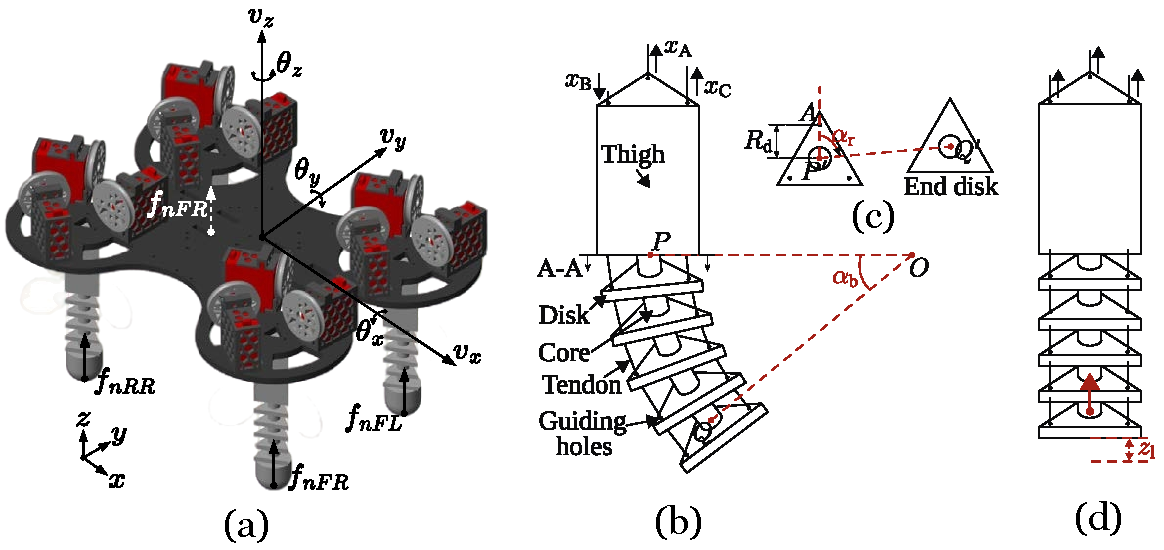
\includegraphics[width=\linewidth]{img/chap3/robots.pdf}
    \caption{Graphical overview of SoftQ and the Compressible Tendon-driven Soft Actuator (CTSA) to drive the robot. (a) Rendered robot with key state notations. (b) The structure and notations of the CTSA. The upper part from section A-A is the rigid thigh for maintaining the actuator length and the lower part is compressible and bendable. The bending angle of the lower part is noted as $\alpha_b$. (c) The top view of the bent CTSA of section A-A. $\alpha_r$ refers to the rotational angle of the CTSA. (d) The CTSA compression is realized by pulling the three tendons by the same amount, with the compression length being noted as $z_l$, originated from Ji et al.\cite{jiSynthesizingOptimalGait2022, jiOmnidirectionalWalkingQuadruped2022}}
    \label{fig:robot}
\end{figure} Notably, the \ac{CTSA}s present a pioneering feature of SoftQ, encompassing soft continuum actuators that facilitate continuous bending or twisting motion throughout their length. Through three motor and \ac{CTSA} systems that evenly distribute forces at radial locations, the robot's four legs attain the capacity for versatile omnidirectional bending\cite{jiOmnidirectionalWalkingQuadruped2022}. Between the \ac{CTSA} and the foot, sensory feedback of contact force is furnished by force sensors attached between them, detecting forces resulting from ground contact, depicted in Figure \ref{fig:actuation}(d). The electrical interface board plays a vital role in this robotic system, facilitating the transmission of both signals and power among motors, microcontrollers, and power sources. Beneath this board, a Raspberry Pi is plugged and mounted by screws, while seamlessly integrated upon it are a STM32 microcontroller and an \ac{IMU}. Additionally, \ac{ToF} sensors are strategically positioned in varying orientations via external hubs, enabling multi-directional sensory input. Accompanying these components, voltage converters and batteries find their placement beneath the panel. Through interconnecting cables, they provide power to the servo motors via the interface board. This distinctive mechanism is visually demonstrated in Figure \ref{fig:robot}, effectively showcasing the robot's versatile and agile locomotion capabilities.

Of particular significance, the architecture of the \ac{CTSA} entails a sequential arrangement of rigid disks and flexible cores, the details of actuation are illustrated in Fig. \ref{fig:actuation}. The interface between the servo motor's shaft and a connected spool serves to convert motor torque into tendon-based force. The end of the tendon are tethered to the spool and the terminal disk of the contiguous continuum structure. Rotation of the spool induces a corresponding change in tendon length. The central position of the spool, designated as position 0, corresponds to the neutral configuration where the actuator assumes a linear form. Positive spool rotations induce tendon retraction, while negative rotations become slack. Tendon-induced forces elicit actuator deformation, with the balance between tendon force and actuator reaction force governing deformation dynamics. The three driven tendons adopt a radial distribution around the actuator's rigid disks, passing through guiding apertures on said disks. The length of the actuators with core and disk structures has been modified, with the upper thigh region reinforced to enhance rigidity. The guiding apertures on rigid disks enable unfettered tendon motion while maintaining positional stability, as depicted in Figure \ref{fig:robot}. This unique attribute eliminates the requirement for discrete joints or segments, thereby contributing to the robot's innate flexibility and agility. To achieve optimal actuator bending while preserving overall robot balance, the servo motor's maximum rotational angle is capped at $\bar{a}_M = \pi/6$, corresponding to a rotational range of [-$\bar{a}_M$,$\bar{a}_M$]. This angular range corresponds to a \ac{PWM} signal interval of [6.67\%, 8.33\%].
\begin{figure}[ht]
    \centering
    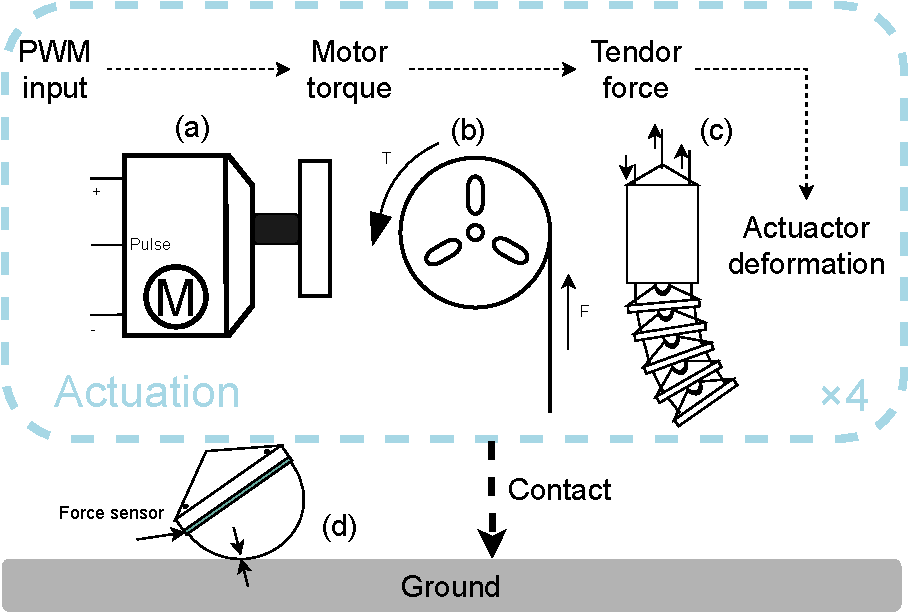
\includegraphics[width=0.9\linewidth]{img/chap3/actuation.pdf}
    \caption{Overview of the quadruped robot's main subsystems enabled by tendon-driven soft actuators. (a) Servo motor converts PWM signal to rotational motions while applying torque exerted on the rotational spool. (b) The spool translates the torque from the servo motor to the traction force in the tendon. (c) The tendon force is applied on the actuator and effectuates its deformation. (d) The actuator's deformation introduces relative motion between the robot's feet and diverse ground conditions, thereby instigating the overall locomotion of the quadruped robot. Reproduced from Ji et al.\cite{ji2022Synthesizing, ji2022Omnidirectional}}
    \label{fig:actuation}
\end{figure}


Furthermore, the inverse kinematics model of \ac{CTSA} using three tendons can be derived through geometric analysis as discussed in \cite{muralidharanSoftQuadrupedRobot2021}, and is expressed as follows:
\begin{equation}
    \begin{aligned}
    x_A &= R_d\alpha_b\cdot{\cos(\alpha_r)} \\
    x_B &= R_d\alpha_b\cdot{\cos(\alpha_r+\frac{2}{3}\pi)} \\
    x_C &= R_d\alpha_b\cdot{\cos(\alpha_r+\frac{4}{3}\pi)}
    \end{aligned}
    \label{eq:value2motor}
\end{equation}

Here, $x_{A,B,C}$ denote the tendon displacement. The positive values of $x_{A,B,C}$ indicate that the tendon pulls the respective actuator end, while negative values signify tendon release and slackening. $R_d$ represents the radius of the circle formed by the three guiding holes on a disk as depicted in Figure \ref{fig:robot}(b). The geometric correlation between $[\alpha_b, \alpha_r]^T$ and $[x_A, x_B, x_C]^T $ can be encapsulated as a function: $g: \mathbb{R}^2 \rightarrow \mathbb{R}^3$. For the described \ac{CTSA}, assuming that the compressed length of the actuator $z_l$ results solely from equal-length pulling of the three tendons, the actuator's total degrees of freedom are established as three: $[\alpha_b, \alpha_r, z_l]^T$. Consequently, the inverse kinematic model of the \ac{CTSA} becomes $f : \mathbb{R}^3 \rightarrow \mathbb{R}^3$:
\begin{equation}
    \begin{bmatrix}x_A\\x_B\\x_C\end{bmatrix} = f(\begin{bmatrix}\alpha_b\\ \alpha_r\\ z_l\end{bmatrix}) = g(\begin{bmatrix}\alpha_b\\ \alpha_r\end{bmatrix}) + z_l\begin{bmatrix}1\\1\\1\end{bmatrix}
    \label{eq:cov2eq}
\end{equation}

The robot design is a sophisticated design for this project, and only part of sensors will be used to guide the optimal gait controller design. The servo motor interfaces with \ac{PWM} signals, generating rotational torque  that is subsequently propagated to downstream subsystems. The utilized servo motor is TS-411MG model from TrackStar, which receives \ac{PWM} signals and rotates the shaft proportionally by a built-in position controller with corresponding sensors. In specific, the robot's feet are equipped with four force sensors each, labelled as \ac{FR}, \ac{FL}, \ac{RR}, and \ac{RL2}. Augmenting the sensing suite are five \ac{ToF} sensors from the Adafruit VL53L1X series, strategically positioned along the robot's four sides and bottom. Additionally, an \ac{IMU} module sourced from Adafruit BNO055 is centrally mounted to facilitate the detection of the robot's pose and localization. For precise localization, the outputs of the \ac{ToF} sensors are fused with the robot's rotational and translational accelerations, as quantified by the \ac{IMU}. This sophisticated data fusion strategy culminates is developed in this thesis for the robot to accurately discern its position and orientation. This augmentation proves particularly advantageous for the successful implementation of \ac{MBRL}. Particularly, certain sensors such as optical cameras and current sensors dedicated to motor control have been mounted on the robot but have not been integrated into the system. This deliberate omission stems from the focused scope of this thesis, which primarily centers on lower-level control aspects and gait coordination.

In order to facilitate the gait control of SoftQ, the robot's local coordinate system has been established utilizing the conventions of the right-hand rule, which is shown in Fig.\ref{fig:robot}(a). In this frame of reference, the $x$ direction denotes the frontal orientation, while the anti-gravity direction aligns with the $z$ direction. For capturing the robot's movements, the roll, pitch, and yaw motions are depicted through the rotational angles of the body center encompassing the three orthogonal axes, designated as $\theta_x$, $\theta_y$, and $\theta_z$. The translational moving velocities are also represented by the movement of the body center in the three directions and are noted as $v_x$, $v_y$ and $v_z$, respectively.

\subsection{Modeling in MathWorks Simulink\texorpdfstring{\textsuperscript{\textregistered}}{(R)}}
\label{sec3.2}
The Simulink model of SoftQ comprises multiple interconnected subsystems, each serving a distinct purpose. These include the motor-driven units, the tendon transmission mechanism, the flexible structure deformation system, and the ground contact subsystem. To model servo behavior in simulation, a \ac{PWM} signals was employed to control the motor, attaching a spool and varying loads and adjusting servo parameters until the deviation between the experimental and the simulation data is minimal. 

As visually depicted in Fig. \ref{fig:robot}, the \ac{CTSA} is constructed through a sequential combination of flexible cores and rigid disks with triangle shapes to retain a high stability and fast fabrication. The three driven tendons are equally distributed at a radial formation around the rigid disks and passed through respective guiding holes placed on the rigid disks, and through the cooperation of three tendons deformation, the legs could realize omnidirectional movement. To model the above soft actuator deformations, the lumped parameter method was applied, where rigid components are applied to build the shape of the cores and the disks while using spring and damper joints for modeling the connections between the cores and disks and enabling the target bending and compression actuator motions. These joints use equivalent stiffness and damping to provide equal response of the entire actuator compared with the flexible segments, only needs to estimate the rigid connecting joint motions with stiffness $k$ and damping $d$ properties in the bending and longitude directions, denoted as $k_B$, $d_B$, $k_L$ and $d_L$ respectively. In the MATLAB Simscape Multibody environment, the continuum structure was modelled using rigid components with telescope joints. Through a series of simulation trials, the equivalent bending properties were estimated to $k_B = 0.0005 N m/deg$ and $d_B = 0.00002 N m/(deg/s)$, and the longitude stiffness and damping were estimated as $k_L = 15000 N/m$ and $d_L = 800 N/(m/s)$.

The tendons simulation was modelled using a belt-cable function within the MATLAB Simscape Multibody environment. This block facilitated a direct connection with the spools and foot, omitting pulleys between the holes on the rigid disks for simulation efficiency. However, recognizing the variance introduced by this omission, a corrective coefficient, $\alpha_c = 1.16$, was introduced. This coefficient adjusts the servo motor's commanded rotation angle ($\theta$) by multiplying it with $\alpha_c$, aiming to bring the actuator's behavior in closer alignment with experimental observations. Furthermore, the use of continuum actuators in the robot, particularly the inclusion of the thigh segment, without the use of pulleys to secure tendon positions, introduces increased model errors due to the simulated detachment of tendons from the thighs. To overcome this issue, adjustments were made by relocating the spools on the servo motor shafts to the lower section of the thigh. This repositioning effectively prevents the tendons from exiting the thigh structure and consequently reduces the model error associated with the lack of pulley configurations. 

The robot is placed on the ground with gravitational forces in the simulation environment. The diverse motions of the four legs result in relative movement with the ground, generating static or dynamic friction that propels the robot's overall movement. It is important to acknowledge that the distinct frictional properties of different ground conditions can lead to varied robot motions. To model the interaction between the quadruped robot's feet and the ground, static and dynamic friction coefficients were specifically determined as $f_s = 0.315$ and $f_d = 0.3$ respectively.

The update period of the RL algorithm is $T_s = 0.05s$ and the simulation model of the soft robot is a continuous-time model. The robot's state representation consists of ten key parameters: the roll, pitch and yaw rotations ($\theta_x$, $\theta_y$, $\theta_z$), translational moving velocities in three axis ($v_x$, $v_y$, $v_z$) and contact force on each feet ($f_{nFL}$, $f_{nFR}$, $f_{nRR}$, $f_{nRL}$). To prevent the robot from falling down or entering unstable states in which the simulation results would be unreliable, termination boundaries are set in the simulation environment. When the robot states meet these termination conditions, the simulation ends before the desired simulation time. The roll and pitch angles of the body center $\theta_x$ and $\theta_y$, are set to rotate less than 0.15 rad, while the bending angle $alph_b$ of all the four legs are set to less than $\pi/3$ rad. 

\section{Experiment Setup}
The experimental setup for Model-Based Reinforcement Learning (MBRL) of the SoftQ quadruped robot encompasses a comprehensive integration of hardware and software components to facilitate the training and evaluation of the robot's locomotion control policies. The SoftQ robot, equipped with its sophisticated subsystems as described earlier, serves as the physical platform for conducting the experiments. 

\begin{figure}[ht]
    \centering
    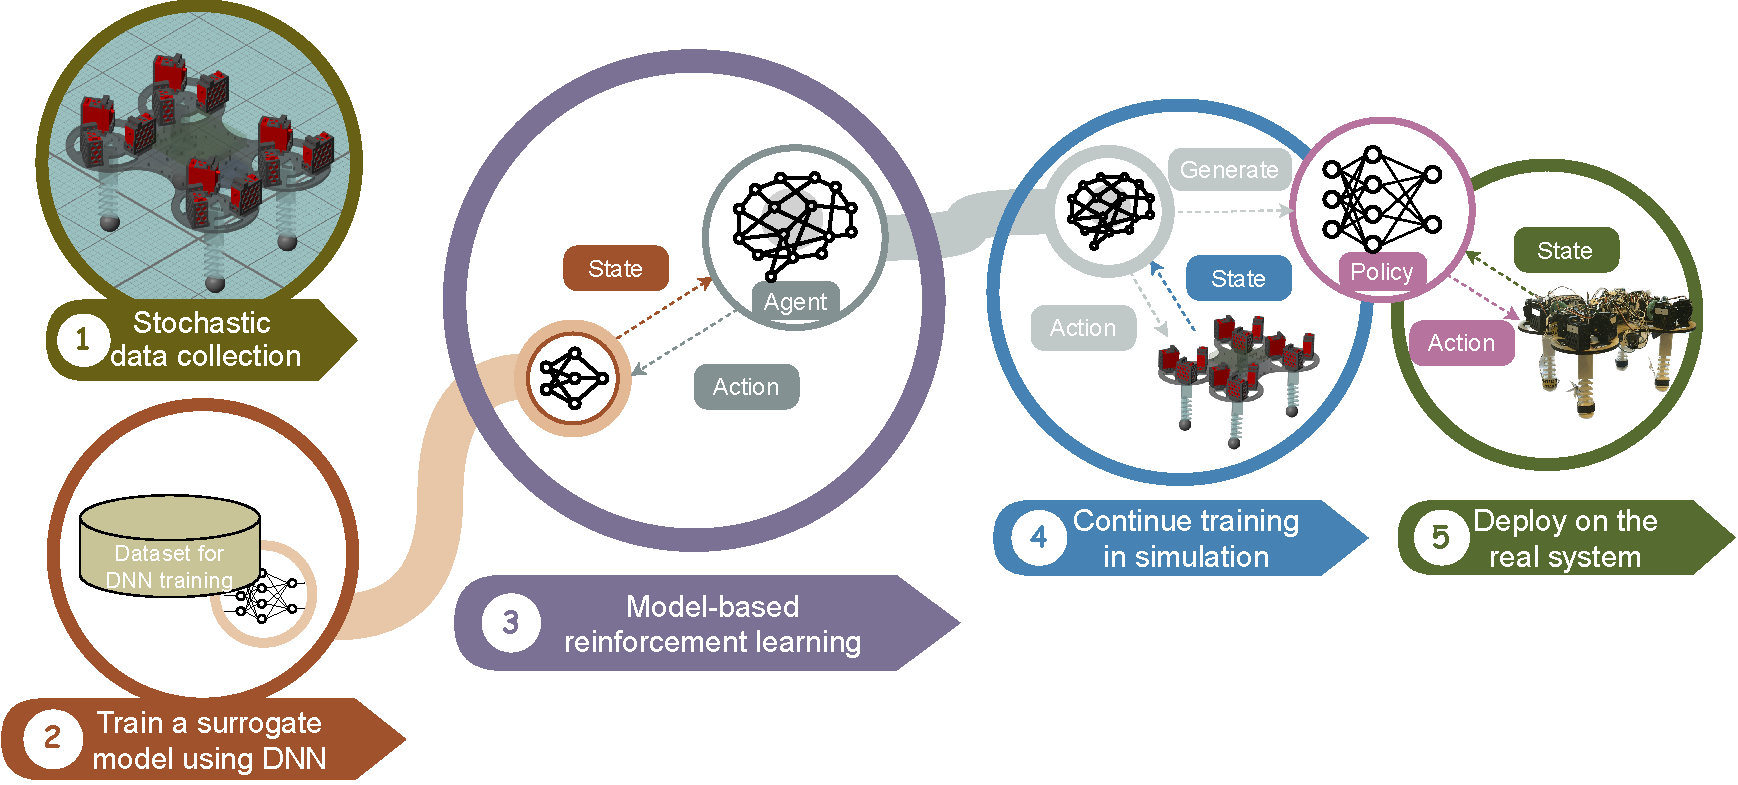
\includegraphics[width=\linewidth]{img/chap3/experiment.pdf}
    \caption{Creating a gait control policy. In the initial step, the physical parameters of the robot was identified and the stochastic actions were simulated in the identification to collect the data. In the subsequent step, an action-observation net was train that models complex robot model dynamics. The third step capitalized on the surrogate models produced in the previous two steps to train a control policy. In the fourth step, the trained control policy was further refined in simulation before deploying on the physical system.}
    \label{fig:exp}
\end{figure}



In this thesis, a practical methodology for autonomously learning and transferring agile and dynamic motor skills for complex and large legged systems were developed. This experimental framework constitutes a pivotal contribution to the field, encapsulated in the schematic representation shown in Figure \ref{fig:exp}. The central premise of this study revolves around the utilization of \ac{RL} to train the gait controller through trial and error, which involves creating a virtual model of the robot and its environment to simulate possible walking behaviors and test the efficacy of various control policies. This approach is motivated by the challenges associated with collecting data in the physical world, which can be time-consuming, costly, and hazardous. By leveraging the benefits of simulation, the training process can generate a large volume of data quickly and inexpensively, allowing for the exploration of a broad range of behaviors and control policies without exposing the physical robot to potential risks.

Central to our approach is the utilization of a surrogate model to facilitate the training of controllers via the principles of deep neural network. This surrogate model serves as a vital intermediary in the training pipeline, mediating the interaction between the RL algorithm and the complex robotic system models. The architecture of surrogate model is embodied in a multi-layer perceptron, which operates as a neural network capable of capturing intricate relationships within the data. This multi-layer perceptron is engineered to process the potential sequence of the robot's states as input and subsequently generate the corresponding actions to be executed by legs as output. This architectural configuration enables the controller with the ability to encapsulate a wide array of state-action dependencies, thereby fostering expedited controller training. Preceding the training of the surrogate model, the collection of stochastic actions and their associated observations is requisite. This data collection process can be time-intensive, but its advantages extend to its reusability for the training of other controllers. This data-driven approach allows for efficient iteration and optimization of the training process, resulting in a control policy that can be effectively applied to the robot.

The trained controller, obtained from the \ac{MBRL} paradigm, would then proceed to a subsequent phase of refinement within the simulation environment. This phase entails simulation-based continuous training, which augments the controller's robustness and efficacy, thereby reducing the reality gap and enhancing its adaptability. Subsequently, the controller that has been refined in the virtual domain is seamlessly transitioned to the physical robotic system. This direct deployment showcases the transferability and generalization capabilities of the acquired motor skills, as the controller is able to translate its learned behaviors from simulation to the tangible real-world setting.

This methodology facilitates the application of deep learning and reinforcement learning techniques to develop a robust and efficient gait controller for the soft quadruped robot. The details of control architecture and the model-based reinforcement learning framework will be shown in the next chapter. During experimentation, the robot undergoes iterative training episodes, where it interacts with its environment to learn locomotion policies. The development environment is listed in Table \ref{tab:env}. Thanks to efficient software implementations, no special computing hardware was needed, such as multi-CPU or multi-GPU servers, for training. All training sessions presented in this thesis were done on a personal computer with one CPU and one GPU, and none lasted more than twenty hours. 
\begin{table}[ht]
    \centering
    \begin{tabular}{ll}
        \toprule
        Component        & Description                             \\\midrule
        Operating System & Windows 10                              \\
        \ac{IDE}              & MATLAB R2021b                           \\
        \ac{CPU}              & Intel(R) Core(TM) i7-4770 CPU @ 3.40GHz \\
        Memory           & 16 GB                                   \\\bottomrule
        \end{tabular}%
    \caption{Development environment for stochastic model}
    \label{tab:env}
\end{table}


The collaboration of these hardware elements significantly enhances both the robot's operational capabilities and its potential for learning. A concise depiction of these hardware constituents is aptly captured in Table \ref{tab:board}, highlighting pivotal components including servo motors, motor control boards, high-level control boards, interface boards, \ac{IMU} units, \ac{ToF} sensors, step-down regulators, and batteries. These components collectively contribute to the robot's ability to perceive its surroundings, execute precise movements, manage power, and establish connections with the external world. It gives rise to a comprehensive robotic system, primed to dynamically interact with its environment and gradually enhance its locomotion capabilities through the exploration of model-based reinforcement learning techniques. In the next chapter, which includes details about control architecture and learning frameworks, the alignment between these hardware components and the research objectives becomes increasingly evident.
\begin{table}[htbp]
    \centering
    \begin{tabular}{lp{10cm}}
        \toprule
        Component        & Description                             \\\midrule
        Servo motor$\times 12$  & TrackStar TS-411MG  (Information from: \href{https://hobbyking.com/en_us/trackstar-ts-411mg-digital-1-10-scale-short-course-steering-servo-11-1kg-0-09sec-57g.html?___store=en_us}{HobbyKing.com}) \\
        Motor control board & STM32G431KB (Information from: \href{https://www.st.com/en/evaluation-tools/nucleo-g431kb.html}{st.com}) \\
        High level control board  & Raspberry Pi4 Model-B standard (Information from: \href{https://www.raspberrypi.com/products/raspberry-pi-4-model-b/}{raspberrypi.com}) \\
        Interface board & Designed by Muralidharan et al. \cite{thorapallimuralidharanContinuumActuatorBased2020} and manufactured by Shenzhen JLC Technology Group Co., Ltd \\
        \ac{IMU} & Adafruit BNO055 9-DoF@I2C (Information from: \href{https://www.bosch-sensortec.com/products/smart-sensors/bno055/#documents}{Adafruit.com}) \\
        \ac{ToF} $\times 5$ & Adafruit VL53L1X Breakout (Information from: \href{https://www.mouser.se/ProductDetail/Pimoroni/PIM373?qs=lc2O%252BfHJPVbu7kI%2FlA0xSg%3D%3D}{mouse.com}) \\
        Step down regulator & LTC3780 DC-DC 5-32V to 1V-30V 10A (Information from: \href{https://www.analog.com/en/products/ltc3780.html#product-overview}{analog.com}) \\
        Battery $\times 2$  & Li-PO 2S 7.4V 30C 1300mAh  (Information from: \href{https://www.batteriexperten.com/sv/artiklar/li-po-2s-74v-30c-1300mah-t-kontakt-vapex.html?gclid=CjwKCAjwoqGnBhAcEiwAwK-OkaSSg7U-01roWZIcyx2yhCrvc7GKyWF5eUhzEE2re9kqi-mnn9GDZBoCB6AQAvD_BwE}{batteriexperten.com})   \\\bottomrule
        \end{tabular}%
    \caption{Hardware components used in the physical robot}
    \label{tab:board}
\end{table}
\chapter{Model-based Reinforcement Learning}
\label{chap4}
\textit{This chapter comprehensively examines the application of data-driven methods to implement \ac{MBRL} for optimal gait control in soft quadruped robots, while also presenting the introduced robot's control architecture.}

\section{Method of Modelling in MBRL}
\subsection{Notation}
The goal of reinforcement learning is to learn a policy that maximizes the cumulative rewards obtained over a sequence of time steps. At each discrete time step denoted by $t$, an agent interacts with its environment. The agent finds itself in a specific state $\mathbf{s}_t$ belonging to the state space $\mathcal{S}$, then performs an action $\mathbf{a}_t$ from the set of possible actions $\mathcal{A}$. Following the action, the agent receives an associated reward $r_t$, which depends on the chosen state and action. Afterward, the agent transitions to a new state $\mathbf{s}_{t+1}$ in a discrete time system. These transitions are determined by the underlying, yet unknown, dynamics function $f$, defined as a mapping from pairs of states and actions to subsequent states $f: (\mathbf{s}_t, \mathbf{a}_t) \rightarrow \mathbf{s}_{t+\Delta t}$. 

In the context of \ac{MBRL}, a surrogate model is developed to approximate the dynamics of the environment. This model is employed to predict the future outcomes of actions and states, aiding the agent in making informed decisions. The learned dynamics function is denoted as $\hat{f}_\theta(\mathbf{s}_t, \mathbf{a}_t)$, and it is parameterized by $\theta$. This learned function accepts the current state $\mathbf{s}_t$ and the action $\mathbf{a}_t$ as inputs and produces an estimate of the future state $\mathbf{s}_{t+1}$ that the agent will encounter after taking the specified action. The parameter $\theta$ captures the characteristics of the learned function, determining its behavior. In this thesis, the chosen approach involves representing the learned dynamics function $\hat{f}_\theta(\mathbf{s}_t, \mathbf{a}_t)$ using a deep neural network. This neural network is designed to capture intricate relationships between the input state and action, allowing it to approximate the complex and often nonlinear dynamics of the environment. 

Before initiating the training process, a dataset $\mathcal{D}$ was assembled through the collection of training samples. These samples were generated by initializing the system with various starting configurations denoted as $\mathbf{s}_0$. Subsequently, random actions $\mathbf{a}_t$ were executed at each time step. These actions were drawn from a probability distribution $p(A)$. The outcomes of these actions were recorded, resulting in a sequence of states $(\mathbf{s}_0, ..., \mathbf{s}_{t-1}, \mathbf{s}_t, \mathbf{s}_{t+1}, ...)$. To ensure equitable treatment of distinct state components encompassing orientations, velocities, and forces, a preprocessing step is enacted. This step encompasses mean subtraction and standard deviation division of the dataset, ultimately leading to data distribution normalization. 

Normalizing the data serves several vital purposes, such as stabilizing training, preventing sensitivity to input variations, mitigating gradient issues, expediting convergence, enhancing generalization, ensuring uniform feature treatment, and acting as a regularization technique. This normalization process is particularly beneficial in cases where state components exhibit significant scale variations, contributing to a more robust and generalized model.

\subsection{Validation}
The surrogate model $\hat{f}_\theta(\mathbf{s}_t, \mathbf{a}_t)$ was subsequently subjected to a training process employing the dataset $\mathcal{D}$. The goal of training was to minimize a specific loss function, specifically half of the \ac{MSE}. is a convention that simplifies the mathematical calculations involved in the training process. This convention simplifies mathematical calculations during the training process without altering the fundamental optimization problem. It streamlines gradient calculations and scales the loss appropriately. The formulation of the loss function is: 
\begin{equation}
    Loss = \frac{1}{|\mathcal{D}|}\sum_{(\mathbf{s}_t,\mathbf{a}_t, \mathbf{s}_{t+1}) \in \mathcal{D}}^\mathcal{D} \frac{1}{2}\lVert \mathbf{s}_{t+1}-\hat{f}_\theta(\mathbf{s}_t, \mathbf{a}_t)\rVert^2
\label{eq:loss}
\end{equation}
where $\lVert\cdot\rVert$ denotes the Euclidean norm. Moreover, the \ac{RMSE} was employed to quantify the accuracy of the predictions made by the surrogate model. This metric provides a comprehensive assessment of the residual errors between the predictions and the true values. The \ac{RMSE} is computed as: 
\begin{equation}
    RMSE = \sqrt{\frac{\sum_{(\mathbf{s}_t,\mathbf{a}_t, \mathbf{s}_{t+1}) \in \mathcal{D}}^\mathcal{D} \frac{1}{2}\lVert \mathbf{s}_{t+1}-\hat{f}_\theta(\mathbf{s}_t, \mathbf{a}_t)\rVert^2}{|\mathcal{D}|}}
    \label{eq:RMSE}
\end{equation}
During the training process utilizing the dataset $\mathcal{D}$, both the \ac{MSE} and \ac{RMSE} in the aforementioned expressions were computed not only on the training dataset but also on a distinct validation dataset $\mathcal{D}_{val}$, which was not part of the training dataset. Additionally, the surrogate model's performance was evaluated on a real walking gait dataset designed human expert, denoted as $\mathcal{D}_{real}$, employing the \ac{NRMSE}:
\begin{equation}
    NRMSE = \sqrt{\frac{1}{\mathcal{D}_{val}}\sum_{(\mathbf{s}_t,\mathbf{a}_t, \mathbf{s}_{t+1}) \in \mathcal{D}_{val}}^{\mathcal{D}_{val}} \lVert \frac{\mathbf{s}_{t+1}-\hat{f}_\theta(\mathbf{s}_t, \mathbf{a}_t)}{max(\mathbf{s}_t) - min(\mathbf{s}_t)}\rVert^2}
    \label{eq:NRMSE}
\end{equation}

While these error metrics offer an estimate of the surrogate model's predictive capability for the next state, it is essential to assess its performance in predicting multi time step model behavior. This is crucial, as the model will be used for long-horizon control. To this end, the validation errors over a span of $T$ steps were computed. This was achieved by employing the learned surrogate model to make multi-step open-loop predictions. For each given sequence $(a_t, ..., a_{t+T})\in\mathcal{D}_{real}$ on the initial starting state $s_0$, a comparison was drawn between the corresponding ground-truth states $(s_t, ..., s_{t+T})\in\mathcal{D}_{real}$ and the multi-step state predictions $(\hat{s}_t, ..., \hat{s}_T)$ generated by the learned surrogate model. This comparison was formulated as:
\begin{equation}
    NRMSE^{T} = \sqrt{\frac{1}{\mathcal{D}_{val}}\sum_{(\mathbf{s}_t,\mathbf{a}_t, \mathbf{s}_{t+1}) \in \mathcal{D}_{val}}^{\mathcal{D}_{val}}\frac{1}{T}\sum_{i=1}^{T}\lVert \frac{\mathbf{s}_{t+i}-\hat{\mathbf{s}}_{t+i}}{max(\mathbf{s}_t) - min(\mathbf{s}_t)}\rVert^2}, 
    \hat{\mathbf{s}}_{t+i} = \begin{cases} 
                        s_t & i=0 \\
                        \hat{f}_\theta(s_t, a_t) & i>0
                    \end{cases}
    \label{eq:NRMSET}
\end{equation}
Furthermore, a further comparison was carried out, involving the ground-truth state $(\mathbf{s}_{t+T})$ and the state prediction derived from the last computed step using the learned surrogate model $(\hat{\mathbf{s}}_{t+T})$. It is used to assess how closely the values of predictions and ground truth are correlated to each other. This comparison incorporated data from a total of $N$ observations and was assessed using the correlation coefficient ($R$), as defined by the following equation:
\begin{equation}
    R=\rho_{val}^{N} = \frac{\sum_{i=1}^{N}(\mathbf{s}_i - \Bar{\mathbf{s}}_i)(\hat{\mathbf{s}}_i-\Bar{\mathbf{s}}_{pred,i})}{\sqrt{\sum_{i=1}^{N}(\mathbf{s}_i - \Bar{\mathbf{s}}_i)^2 \sum_{i=1}^{N}(\hat{\mathbf{s}}_i-\Bar{\mathbf{s}}_{pred,i})^2}}
    \label{eq:R}
\end{equation}
where $\Bar{\mathbf{s}}_{pred,i}$ represents the mean prediction of the surrogate model for state $\mathbf{s}_i$ based on the actions $\mathbf{a}_i$ and is calculated as: $\Bar{\mathbf{s}}_{pred,i} = \frac{1}{n}\sum_{i=1}^{n}\hat{f}_\theta(\mathbf{s}_i, \mathbf{a}_i)$ 

Importantly, the $T$-step validation procedure was exclusively utilized for result analysis and was not employed during the actual training process.

\section{Neural Networks Design}
\label{sec:NN_design}
When considering the creation of a surrogate model to expedite the RL training process, as discussed in Chapter \ref{chap2}, \ac{ANN} comes to the forefront of the thoughts due to their inherent capacity to capture complex relationships within data and provide an efficient approximation of underlying dynamics\cite{zouOverviewArtificialNeural2009}. As highlighted, there exist multiple viable approaches within the realm of \ac{ANN}s, such as typical \ac{DNN}, \ac{RNN} and \ac{CNN}. Although \ac{CNN}  are a subset of feedforward neural networks, their convolutional layers are specifically tailored to discern spatial patterns and features within multidimensional and local receptive fields. This attribute renders them particularly suited for analyzing the influence of actions on subsequent states in a structured manner. However, given that the model at hand pertains to complex temporal relationships, the utilization of \ac{CNN} is not suitable within the scope of this thesis.

Belongs to \ac{ANN}, a typical \ac{DNN} consists of interconnected layers of artificial neurons, including the input layer, hidden layers, and output layer, which builds up the world of artificial intelligence and offers a straightforward design approach. The input layer receives raw data and transfers it to subsequent layers. The hidden layers undertake intermediate computations, employing activation functions to extract intricate features from the data. The output layer produces the final network output based on the assigned task, such as classification or regression. The design of the hidden layers can be meticulously tailored to accommodate various tasks, ensuring adaptability and versatility in tackling diverse computational challenges. 

Emerging as a distinct architecture within the realm of \ac{ANN}, \ac{RNN}s present a distinctive architecture. Setting them apart from the conventional feedforward neural networks, \ac{RNN}s incorporate loops within their structure, thereby enabling the assimilation of sequential and temporal information. This unique characteristic renders \ac{RNN}s especially adept at handling tasks characterized by sequences, time series data, and other dynamic patterns\cite{liptonCriticalReviewRecurrent2015}. Notably, each neuron within an \ac{RNN} not only processes the immediate input but also taps into information from preceding time steps, resulting in the creation of an internal memory mechanism. This inherent recurrence empowers \ac{RNN}s to effectively capture dependencies evolving over time and to manage sequences of varying lengths\cite{sherstinskyFundamentalsRecurrentNeural2020}. Given these attributes, \ac{RNN}s are considered a choice for capturing the complex dynamics between actions and observations in time series data.

\subsection{Neural Network Architecture}
Continuing with the discussion of neural network architecture, it is important to underscore the significance of selecting an appropriate model for the specific task at hand. \ac{DNN} serve as a foundational architecture in the realm of artificial neural networks. They are characterized by an intricate interconnection of layers consisting of artificial neurons, including input, hidden, and output layers.

In the context of DNNs, raw data is initially received at the input layer and subsequently propagated through the network's layers. The intermediate computations occur within the hidden layers, which are strategically positioned between the input and output layers. These computations involve the application of activation functions at each pair of hidden layers. A commonly used activation function is \ac{ReLU}\cite{sunFormalVerificationStochastic2022}, known for introducing non-linearity by transforming negative values to zero while preserving positive values through element-wise activation. 

A fundamental component within DNNs is the fully connected layer, also referred to as the dense layer\cite{goodfellowDeepLearning2016}. This layer's distinguishing feature is that every neuron within it is interconnected with each neuron in the preceding and succeeding layers. This interconnectedness allows for comprehensive feature extraction and transformation. Neurons in the fully connected layer apply a linear transformation to the input vector using weight matrices. Subsequently, a non-linear activation function, denoted as $f$, is applied to the product: $y_{jk}(x)=h\left(\sum_{i=1}^{n_H} w_{j k} x_i+w_{j0}\right)$. Finally, the output layer generates the network's ultimate output, tailored to the specific regression task at hand. The structural arrangement of a DNN is visually depicted in Fig. \ref{fig:NN}.
\tikzset{%
  every neuron/.style={
    circle,
    draw,
    minimum size=0.5cm
  },
  neuron missing/.style={
    draw=none, 
    scale=3,
    text height=0.333cm,
    execute at begin node=\color{black}$\vdots$
  },
}

\begin{figure}[ht]
\centering
    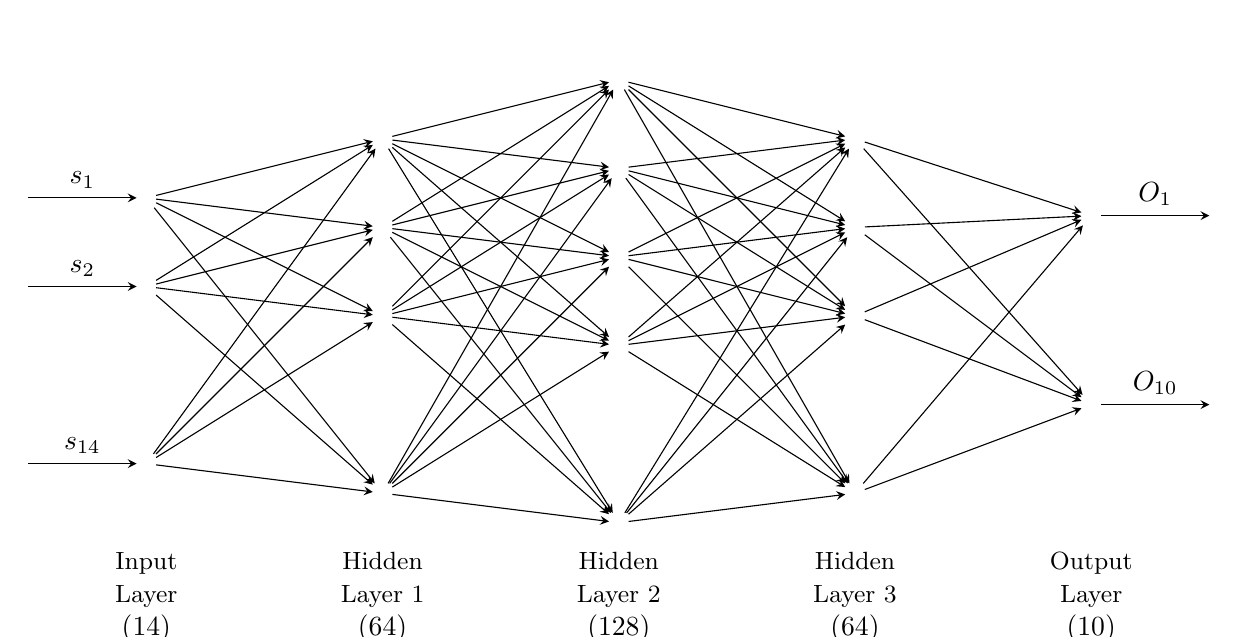
\begin{tikzpicture}[x=1.5cm, y=1.5cm, >=stealth, auto]
    
        \foreach \m/\l [count=\y] in {1,2,missing,3}
          \node [every neuron/.try, neuron \m/.try] (input-\m) at (0,2-\y*.75) {};
        \foreach \m [count=\y] in {1,2,3,missing,4}
          \node [every neuron/.try, neuron \m/.try ] (hidden1-\m) at (2,2.5-\y*0.75) {};
        \foreach \m [count=\y] in {1,2,3,4,missing,5}
          \node [every neuron/.try, neuron \m/.try ] (hidden2-\m) at (4,3-\y*0.75) {};
        \foreach \m [count=\y] in {1,2,3,missing,4}
          \node [every neuron/.try, neuron \m/.try ] (hidden3-\m) at (6,2.5-\y*.75) {};
        \foreach \m [count=\y] in {1,missing,2}
          \node [every neuron/.try, neuron \m/.try ] (output-\m) at (8,1.9-\y*.8) {};
        \foreach \l [count=\i] in {1,2,14}
          \draw [<-] (input-\i) -- ++(-1,0)
            node [above, midway] {$s_{\l}$};
        \foreach \l [count=\i] in {1,10}
          \draw [->] (output-\i) -- ++(1,0)
            node [above, midway] {$O_{\l}$};
        \foreach \i in {1,...,3}
          \foreach \j in {1,...,4}
            \draw [->] (input-\i) -- (hidden1-\j);
        \foreach \i in {1,...,4}
          \foreach \j in {1,...,5}
            \draw [->] (hidden1-\i) -- (hidden2-\j);
        \foreach \i in {1,...,5}
          \foreach \j in {1,...,4}
            \draw [->] (hidden2-\i) -- (hidden3-\j);
        \foreach \i in {1,...,4}
          \foreach \j in {1,...,2}
            \draw [->] (hidden3-\i) -- (output-\j);
        \foreach \l [count=\x from 0] in {\small Input \\\small Layer\\(14) ,\small Hidden \\\small Layer 1\\(64), \small Hidden \\\small Layer 2\\(128), \small Hidden \\\small Layer 3\\(64), \small Output \\\small Layer\\(10)}
          \node [align=center, below, yshift=-5.5cm] at (\x*2,2) {\l};
    \end{tikzpicture}
    \caption{Neural network structure of surrogate model}
    \label{fig:NN}
\end{figure}
        % \foreach \l [count=\i] in {1,2,3,64}
        %   \node [above] at (hidden1-\i.north) {$H_{1,\l}$};
        % \foreach \l [count=\i] in {1,2,3,4,128}
        %   \node [above] at (hidden2-\i.north) {$H_{2,\l}$};
        % \foreach \l [count=\i] in {1,2,3,64}
        %   \node [above] at (hidden3-\i.north) {$H_{3,\l}$};

DNNs are particularly adept at capturing intricate and complex relationships within data\cite{goodfellowDeepLearning2016}, making them well-suited for a wide range of applications, including image recognition, natural language processing, and more. In contrast, \ac{RNN}, characterized by loops in their structure, are ideal for handling sequential and temporal data, incorporating information from previous time steps to model temporal dynamics\cite{liptonCriticalReviewRecurrent2015}. Each neuron within an RNN not only processes the current input but also incorporates information from previous time steps. This inherent recurrence equips RNNs to capture and model temporal dynamics, which is essential for scenarios where actions influence subsequent states over time\cite{sherstinskyFundamentalsRecurrentNeural2020}. RNNs employ loops to create a feedback mechanism where the output from one step becomes the input for the next. This cyclic connectivity enables RNNs to maintain a form of memory across different time steps\cite{liptonCriticalReviewRecurrent2015}. As an evolution of the RNN architecture, \ac{LSTM} layers incorporate specialized memory cells and gating mechanisms that enable them to selectively retain or forget information over extended sequences\cite{yuReviewRecurrentNeural2019}. These mechanisms regulate the flow of information through the network, allowing it to selectively remember or forget information over longer sequences.
\tikzset{%
  every neuron/.style={
    circle,
    draw,
    minimum size=0.5cm
  },
  neuron missing/.style={
    draw=none, 
    scale=3,
    text height=0.333cm,
    execute at begin node=\color{black}$\vdots$
  },
  rect neuron/.style={ % Define the style for rectangle nodes
  rectangle,
  draw,
  minimum size=0.5cm,
  align=center, 
  },
  cross/.style={
    path picture={
      \draw[black]
        (path picture bounding box.south east) -- (path picture bounding box.north west)
        (path picture bounding box.south west) -- (path picture bounding box.north east);
    }
  },
}

\begin{figure}[ht]
\centering
    \begin{tikzpicture}[x=1.5cm, y=1.5cm, >=stealth, auto, scale=0.8]
        \foreach \m/\l [count=\y] in {1,2,missing,3}
          \node [every neuron/.try, neuron \m/.try] (input-\m) at (0,2-\y*.75) {};
        \foreach \m [count=\y] in {1,2,3,missing,4}
          \node [every neuron/.try, neuron \m/.try ] (hidden1-\m) at (2,2.5-\y*0.75) {};
        \node [rect neuron/.try, neuron 1/.try] (hidden2-1) at (4,3-1*0.75) {LSTM};
        \node [rect neuron/.try, neuron 2/.try] (hidden2-2) at (4,3-2*0.75) {LSTM};
        \node [rect neuron/.try, neuron 3/.try] (hidden2-3) at (4,3-3*0.75) {LSTM};
        \node [rect neuron/.try, neuron 4/.try] (hidden2-4) at (4,3-4*0.75) {LSTM};
        \node [rect neuron/.try, neuron missing/.try] (hidden2-missing) at (4,3-5*0.75) {};
        \node [rect neuron/.try, neuron 5/.try] (hidden2-5) at (4,3-6*0.75) {LSTM};

        % Dropout Layer
        \node [every neuron/.try, neuron 1/.try ] (dropout-1) at (6,2.5-2*0.75) {};
        \node [every neuron/.try, neuron missing/.try ] (dropout-missing) at (6,2.5-4*0.75) {};
        \node [every neuron/.try, neuron 1/.try ] (dropout-2) at (6,2.5-5*0.75) {};
        \node [every neuron/.try, neuron 1/.try, cross] (dropouted-1) at (6,2.5-1*0.75) {};
        \node [every neuron/.try, neuron 1/.try, cross] (dropouted-2) at (6,2.5-3*0.75) {};
        \foreach \m [count=\y] in {1,missing,2}
          \node [every neuron/.try, neuron \m/.try] (output-\m) at (8,1.9-\y*.8) {};
        \foreach \l [count=\i] in {1,2,14}
          \draw [<-] (input-\i) -- ++(-1,0)
            node [above, midway] {$s_{\l}$};
        \foreach \l [count=\i] in {1,10}
          \draw [->] (output-\i) -- ++(1,0)
            node [above, midway] {$O_{\l}$};
    
        \foreach \i in {1,...,3}
          \foreach \j in {1,...,4}
            \draw [->] (input-\i) -- (hidden1-\j);
        \foreach \i in {1,...,4}
          \foreach \j in {1,...,5}
            \draw [->] (hidden1-\i) -- (hidden2-\j);
        \foreach \i in {1,...,5}
          \foreach \j in {1,...,2}
            \draw [->] (hidden2-\i) -- (dropout-\j);
        \foreach \i in {1,...,2}
          \foreach \j in {1,...,2}
            \draw [->] (dropout-\i) -- (output-\j);
        \foreach \l [count=\x from 0] in {\small Input \\\small Layer\\(14), \small Fully connected \\\small Layer (64), \small LSTM \\\small Layer \\(100), Dropout layer \\(0.5), \small Output \\\small Layer\\(10)}
          \node [align=center, below, yshift=-4.5cm] at (\x*2,2) {\l};
    \end{tikzpicture}
    \caption{\ac{LSTM} \ac{RNN} Architecture. The figure illustrates the architecture of an LSTM-based  RNN. The initial layer comprises the input data, followed by a fully connected layer featuring 64 neurons. Subsequently, the fully connected layer is seamlessly activated by a \ac{ReLU} function before connected to a bidirectional LSTM layer with 100 hidden units. A Dropout layer with 0.5 probability is strategically incorporated before the output layers. }
    \label{fig:lstmstruct}
\end{figure}
        % \foreach \l [count=\i] in {1,2,3,64}
        %   \node [above] at (hidden1-\i.north) {$H_{1,\l}$};
        % \foreach \l [count=\i] in {1,2,3,4,128}
        %   \node [above] at (hidden2-\i.north) {$H_{2,\l}$};
        % \foreach \l [count=\i] in {1,2,3,64}
        %   \node [above] at (hidden3-\i.north) {$H_{3,\l}$};

In the context of the SoftQ surrogate model, a bidirectional LSTM architecture is also adopted, involving two distinct LSTM layers. The first layer processes the sequence in the traditional forward direction, while the second layer processes it in reverse. This bidirectional approach enhances the model's ability to capture bidirectional dependencies within the data. The architecture of the bidirectional LSTM RNN is visually depicted in Fig. \ref{fig:lstmstruct}. In addition to the LSTM layer, a dropout layer with a dropout rate of 50\% is incorporated into the architecture to enhance robustness and generalization capabilities. The dropout layer is a regularization technique that helps prevent overfitting by randomly setting a portion of the input neurons to zero during training.

With the architectural groundwork laid, 15\% of the training data was reserved for validation purposes, and the loss and \ac{RMSE} of the training is shown in Fig. \ref{fig:train2net}(a) and (c). Following this validation stage, the network was evaluated with some manual trot gait test data, the evaluation results are shown in Fig. \ref{fig:comp2net}.

\subsection{Optimization Algorithms}
Furthermore, it is essential to emphasize that alongside architectural considerations, the choice of optimization algorithms holds significant importance before the commencement of the training process. These algorithms steer the iterative parameter updates that guide the model towards convergence. Popular optimization algorithms include \ac{SGDM}\cite{liuImprovedAnalysisStochastic2020}, \ac{Adam}\cite{zhangImprovedAdamOptimizer2018}, and \ac{RMSProp}\cite{liDeepConvolutionGated2021}. These algorithms adjust the weights of the model based on the gradients of the loss function with respect to the parameters. They help to guide the model towards finding optimal parameter values that minimize the loss function.

\ac{SGDM} augments the standard Stochastic Gradient Descent (SGD) by introducing a momentum term. This term incorporates the weighted average of the previous gradients to determine the direction of the parameter updates. This addition imparts momentum to the optimization process, allowing for smoother convergence by reducing the oscillations that can occur during gradient updates\cite{zhangComputerVisionbasedTree2021}. The momentum term helps to accelerate the movement along shallow directions while dampening oscillations in steep directions. 

\ac{Adam} is an optimization algorithm that combines the advantages of both momentum-based methods and adaptive learning rates. It maintains exponentially decaying moving averages of both past gradients and past squared gradients\cite{zhangRobotGraspingMethod2021}. These moving averages are used to compute adaptive learning rates for individual parameters. Additionally, \ac{Adam} employs bias correction mechanisms to counteract potential bias towards zero at the beginning of training. By adjusting the learning rates dynamically based on the historical gradients, \ac{Adam} enhances convergence speed and adaptability across varying gradients\cite{zhangRobotGraspingMethod2021}.

\ac{RMSProp} is an optimization technique designed to address the challenges of learning rate selection in \ac{SGDM}. It maintains an exponentially decaying average of squared gradients for each parameter. The learning rate is then divided by the square root of this average, which normalizes the learning rate by the historical gradient magnitudes. This adaptive learning rate adjustment helps to mitigate the problem of diminishing or exploding gradients\cite{escobar-naranjoSelfsupervisedLearningApproach2023}.

\begin{figure}[htb]
    \centering
    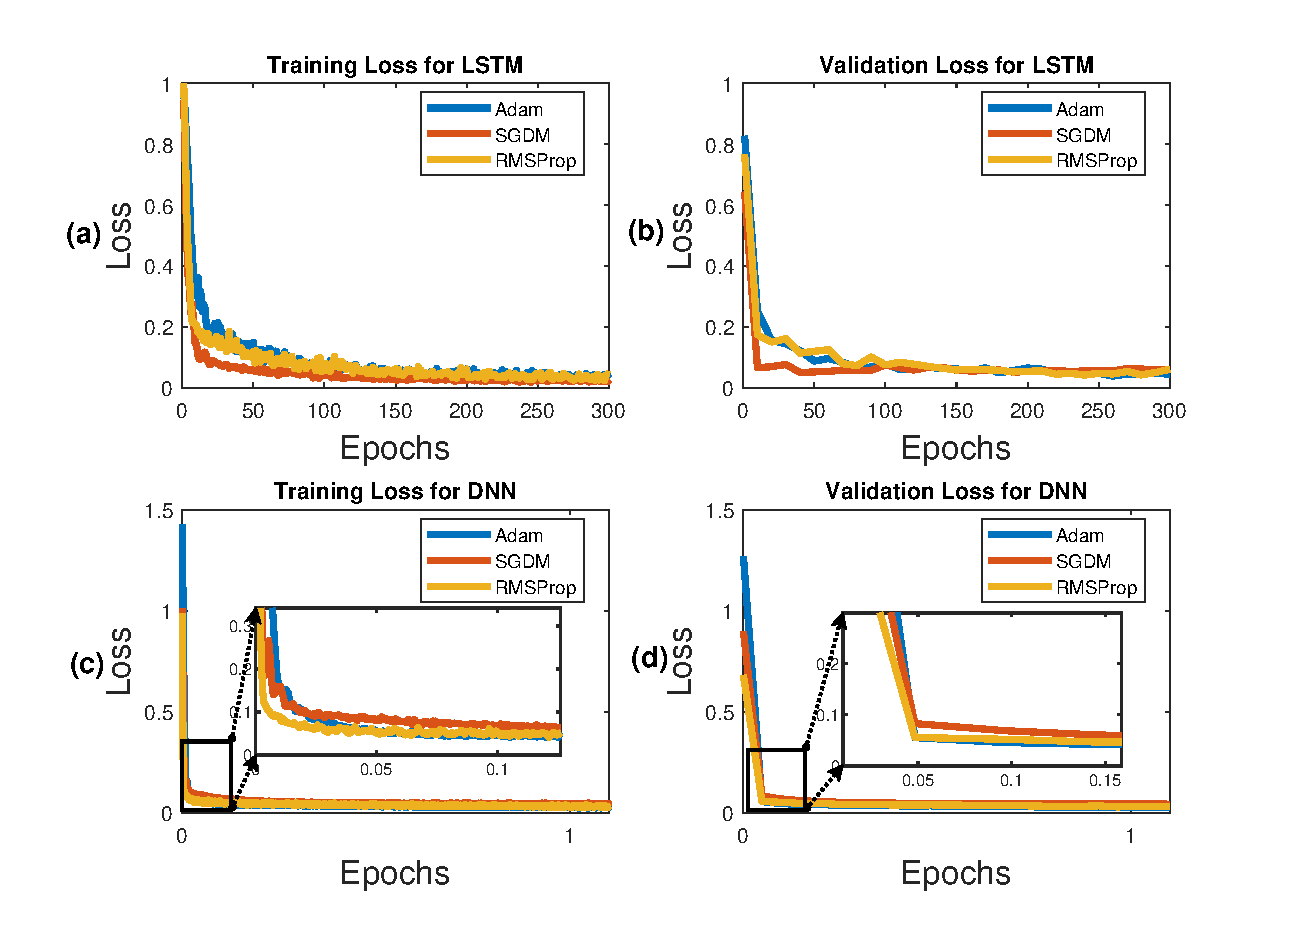
\includegraphics[width=\linewidth]{img/chap4/comp_op.eps}
    \caption{Comparison of Training Trajectories with Different Optimization Algorithms. The figure illustrates the training trajectories of two applied architectures while employing three different optimization algorithms: \ac{SGDM}, \ac{Adam}, \ac{RMSProp}. (a) Training loss and (b) validation loss for the bidirectional \ac{LSTM}-based \ac{RNN} architecture, (c) training loss (d) validation loss for the \ac{DNN} architecture.}
    \label{fig:comp3op}
\end{figure}

By implementing all three optimization algorithms in two networks, a comprehensive exploration was undertaken to discern the most suitable optimization strategy for the training of the surrogate model. This comprehensive approach facilitated a comprehensive assessment of each algorithm's impact on the training process and subsequent model performance. Specifically, the training was performed on both the bidirectional LSTM-RNN and DNN architectures, maintaining a consistent learning rate of 0.001. The training data was shuffled at the end of each epoch, and a mini-batch size of 512 was utilized. The training trajectories of the bidirectional LSTM-RNN and DNN networks, encompassing the utilization of the three optimization algorithms, are visually depicted in Figure \ref{fig:comp3op}. 

For the bidirectional LSTM-based RNN architecture, SGDM is the emerged as the optimal choice due to its remarkable ability to achieve the lowest training loss and converge rapidly. It exhibited both the fastest convergence and the least training loss among the evaluated optimization algorithms. In contrast, for the DNN architecture, Adam optimization took the lead. Adam demonstrated superior performance by learning rapidly and converging to the lowest loss values, both in validation and training. Its ability to efficiently navigate the DNN's training dynamics underscores its suitability for this architecture. Notably, all three optimization algorithms proved to be stable options for training this architecture effectively.

\subsection{Network Validation}
Nonetheless, when comparing the training performance of the bidirectional LSTM-based RNN architecture and the DNN architecture, as illustrated in Figure \ref{fig:train2net}, it becomes evident that the DNN architecture exhibits greater efficiency in terms of data utilization. Notably, the DNN showcases the capability to converge to a lower loss while achieving a reduced \ac{NRMSE}. This underscores the DNN's efficiency in leveraging the provided data and achieving enhanced predictive accuracy with a more compact loss function. Furthermore, evaluated against the real expert trot gait simulation data, the bidirectional LSTM-based RNN architecture achieves an NRMSE of approximately 0.61 for single step prediction, whereas the DNN attains a significantly lower NRMSE of around 0.26. This substantial divergence in NRMSE values highlights the DNN's proficiency in making more accurate predictions on these test cases. A more comprehensive review of the single-step predictions, as compared to the expert trot simulation data, can be observed in Figure \ref{fig:lstm_test} and Figure \ref{fig:DNN_test} in the Appendix.

\begin{figure}[H]
    \centering
    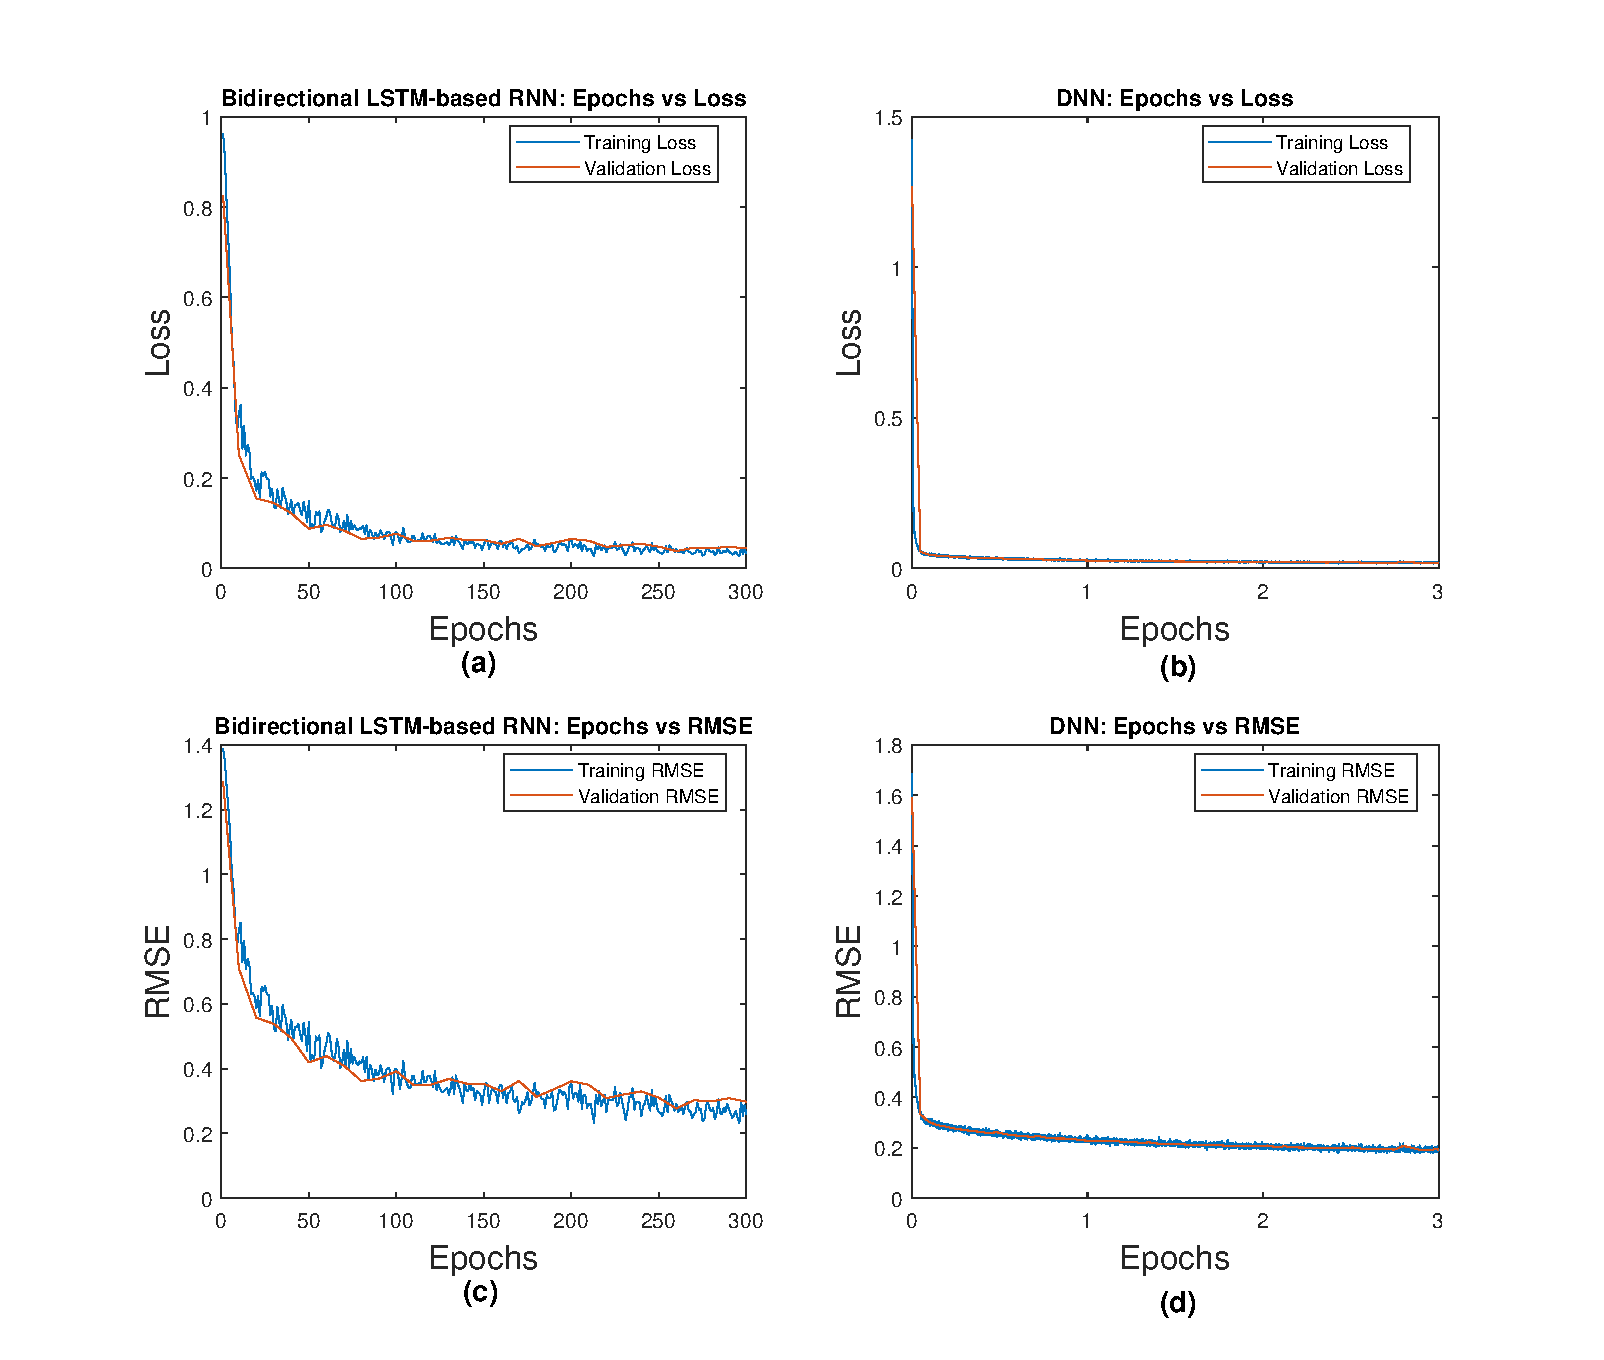
\includegraphics[width=\linewidth]{img/chap4/train_result.eps}
    \caption{Training of bidirectional LSTM-RNN architecture and DNN architecture. (a)-(b) Loss vs epoch for model training with bidirectional LSTM-based and DNN model; (c)-(d) RMSE vs epoch for model training with bidirectional LSTM-based and DNN model.}
    \label{fig:train2net}
\end{figure}

In addition, an evaluation of the long-term predictions produced by both architectures, as illustrated in Figure \ref{fig:comp2net}, reveals valuable insights. The average correlation coefficient ($R$) for the DNN architecture's single-step predictions exceeded 0.9, maintaining a commendable level of above 0.76 even for predictions spanning 10 seconds. While there was a slight increase in the \ac{NRMSE} for the DNN architecture from 0.26 to 0.35, the \ac{NRMSE} remained relatively stable in the case of the bidirectional LSTM-based RNN. Additionally, it was also observed from the correlation coefficient ($R$) of different prediction steps that the bidirectional LSTM-based RNN architecture did not exhibit substantial drops, demonstrating its stability in predicting long-term and time-series data with consistency. On the other hand, the bidirectional LSTM-based RNN architecture demonstrated a single-step correlation coefficient ($R$) of around 0.64 and an \ac{NRMSE} of approximately 0.62. For long-term predictions, these metrics do not surpass those achieved by the DNN architecture, indicating its limited ability to predict future states with high accuracy. 
\begin{figure}[htb]
    \centering
    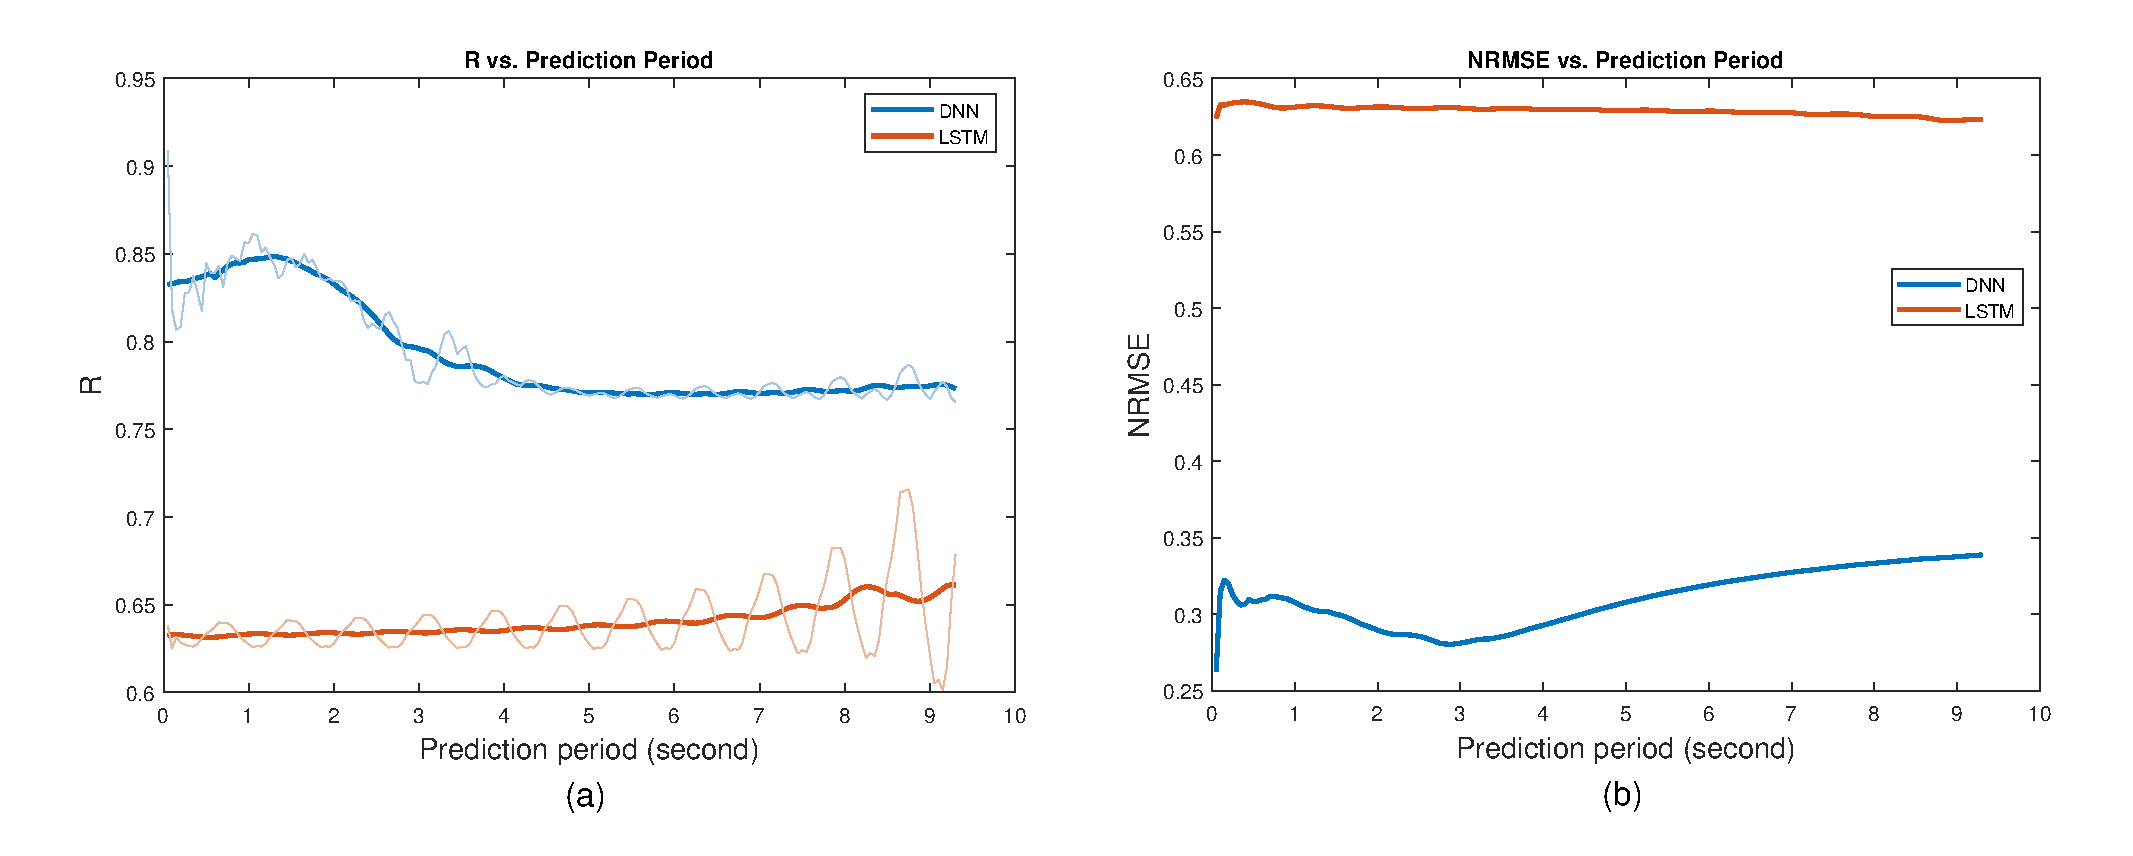
\includegraphics[width=\linewidth]{img/chap4/long2net.eps}
    \caption{Comparison of Long-Term Predictions by Some Expert Gait Data $\mathcal{D}_{real}$. (a) This figure illustrates the average correlation coefficient ($R$) of long-term predictions between the DNN architecture and the bidirectional LSTM-based RNN architecture. (b) This figure shows the \ac{NRMSE} of long-term predictions between the DNN architecture and the bidirectional LSTM-based RNN architecture.}
    \label{fig:comp2net}
\end{figure}

LSTM is designed to capture long-term dependencies in sequential data, which can introduce unnecessary complexity when applied to problems with less pronounced sequential patterns. In contrast, DNNs are simpler and may be better suited for situations where data relationships are not strongly sequential. The underlying dynamics of the environment may involve complex and nonlinear relationships. DNNs are well-suited for capturing such intricate patterns, as they can adapt their internal representations to accommodate nonlinearities. While LSTM is a powerful choice for tasks with strong sequential dependencies, it may not be the best fit for problems where data relationships are less sequential. In this particular case, the characteristics of the problem favored the DNN architecture. LSTM, while proficient in handling sequential dependencies, may not excel in capturing these nonlinear relationships. The DNN's efficiency, simplicity, ability to capture nonlinear patterns, and stability in long-term predictions made it the preferred architecture for this particular task of surrogate model training. Therefore, the DNN architecture optimized with the Adam optimization algorithm emerges as a promising choice for surrogate model training.

\subsection{Dataset Size}
The neural network's architecture, as discussed earlier, provides the framework for representing the complex relationships within the soft quadruped robot's behavior. However, the size of dataset remains a critical factor in enabling the neural network to learn effectively and achieve high estimation accuracy. The dataset's size is defined as a sequence of data, where each sequence data refers to the data collected during a sampling session that occurs without any failures. This definition is established to guarantee the consistency and reliability of the data employed in the neural network's training.

A sufficiently large dataset is essential as it provides the neural network with a diverse set of examples that encompass various scenarios and conditions. This diversity allows the network to generalize well and effectively capture the underlying relationships inherent in the dynamics of the soft quadruped robot. The consequence of having a small dataset is the risk of overfitting, where the network memorizes the training examples but does not truly comprehend the underlying patterns. Conversely, a larger dataset should aid the network in learning these underlying patterns more comprehensively and reduce the risk of overfitting. 

In Figure \ref{fig:datasize}, the average results of 5 long-prediction tests with different dataset size are shown. The correlation coefficient ($R$) remains similar at the single-step prediction level, but for long-term prediction, R increases significantly as the dataset size grows from 20 to around 220 sequences of data. It is worth noting that our analysis identifies oscillations in the correlation coefficient ($R$). These oscillations can be attributed to the presence of an oscillation gait pattern within the data. This gait pattern introduces fluctuations in the predictions at different time steps. Furthermore, we observe that such oscillations are more pronounced when using LSTM networks. This behavior can be attributed to the LSTM's focus on capturing long-term dynamics, potentially overlooking instantaneous dynamics.

In addition to the correlation coefficient, the prediction accuracy was also assessed using \ac{NRMSE}. The findings reveal a consistent trend: the NRMSE decreases as the dataset size grows from 20 sequences to around 280 sequences. These observations indicate that a larger dataset contributes to improved generalization, enhancing the network's ability to accurately estimate the behavior of the soft quadruped robot across a broader range of situations, including those has not encountered during sampling. This becomes particularly crucial when deploying the surrogate model in real-world scenarios where conditions may vary.

However, it is noteworthy that the trend reverses after 300 sequences of data and worsens further with 3000 sequences of data. The reason for the decline in performance with more data could be attributed to the fact that the random action data collected may not adequately characterize the useful information about the robot's dynamics. This could be due to the imbalanced distribution of data, with fewer samples representing high walking velocity, leading to the diminishing returns of adding more data in this form.
\begin{figure}[htb]
    \centering
    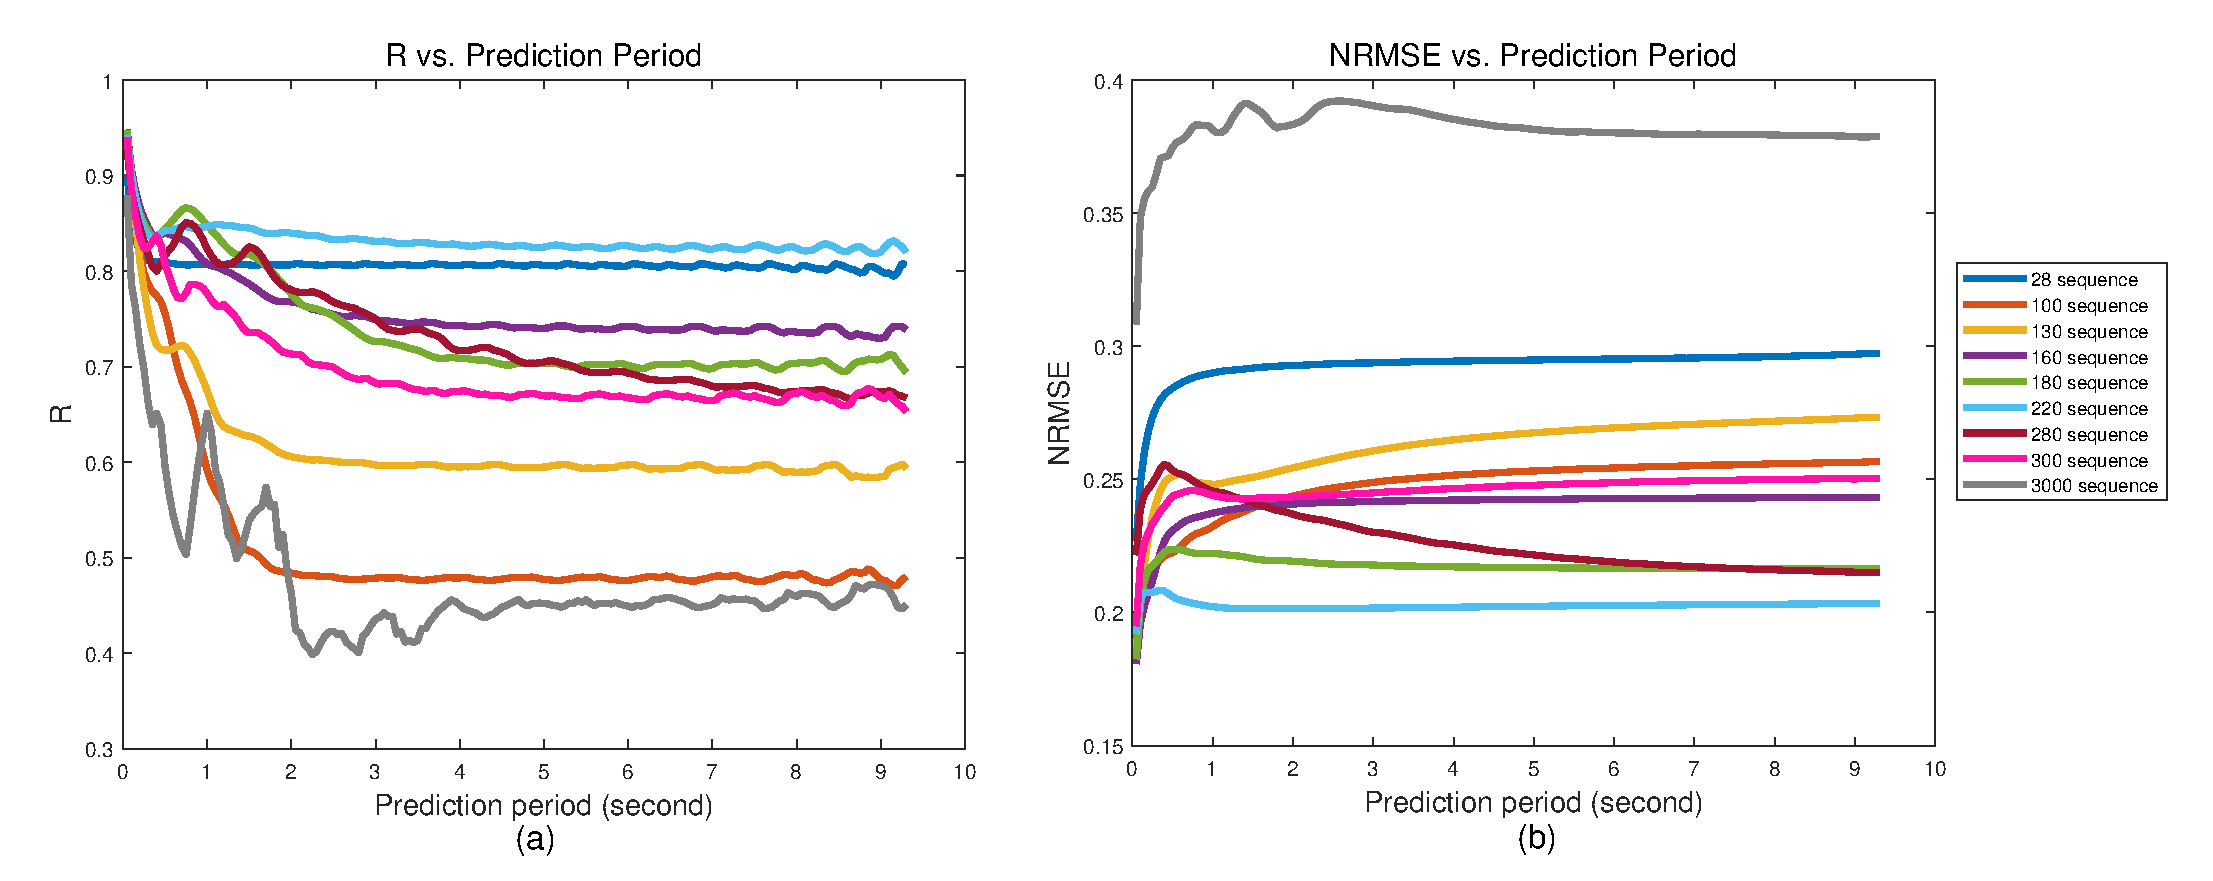
\includegraphics[width=\linewidth]{img/chap4/datasize.eps}
    \caption{Comparison of Different Data Size of Dataset $\mathcal{D}$ in Long-Term Predictions using some expert trot gait data. (a) This figure illustrates the average correlation coefficient ($R$) of long-term predictions between the DNN architecture and the bidirectional LSTM-based RNN architecture. (b) This figure shows the \ac{NRMSE} of long-term predictions between the DNN architecture and the bidirectional LSTM-based RNN architecture.}
    \label{fig:datasize}
\end{figure}

It is crucial to strike a balance between dataset size and the associated computational resources and time required for training. Collecting and curating a substantial dataset demands significant effort and resources, and training a neural network on a large dataset can be computationally intensive. Therefore, careful consideration is required to determine an appropriate dataset size that aligns with the available resources while still achieving the desired level of accuracy and generalization. Based on these observations, selecting a dataset size approximately 20 times the dimensions of the observation data seems to strike a reasonable balance for the surrogate model in this thesis, which means about 200 sequences of data in this thesis.

\section{Model-based RL Algorithm}
After successfully training the surrogate model, the next phase of this thesis involves the application of \ac{MBRL} algorithms to further advance the research objectives. As previously discussed in Chapter \ref{chap2}, the \ac{SAC} algorithm has been selected due to its advantages in promoting efficient exploration and its compatibility with continuous action spaces. 

SAC addresses the challenge of dealing with continuous action spaces by incorporating an actor network that explicitly represents the policy function. This actor network is parameterized to output a probability distribution over actions, typically modeled as a Gaussian distribution with mean and standard deviation. SAC learns both the Q-function and the policy (actor) simultaneously through a combination of entropy-regularized policy optimization and Q-value estimation. In Figure \ref{fig:SAC}, an overview of this approach to learn a walking gait controller for a quadruped robot using the SAC algorithm is presented.
\begin{figure}[htb]
    \centering
    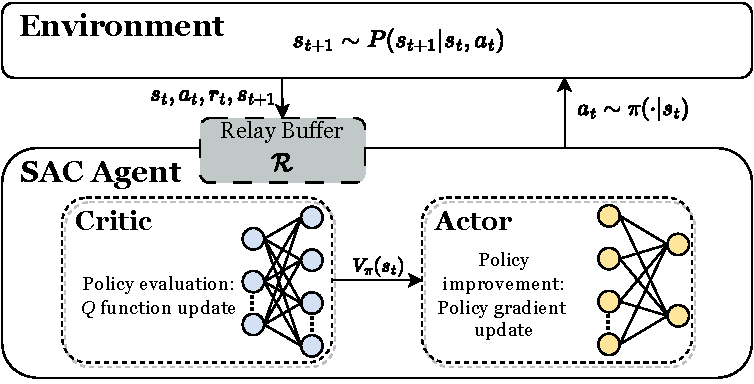
\includegraphics[width=0.9\linewidth]{img/chap4/SAC.pdf}
    \caption{Schematic of the Soft Actor Critic (SAC) method. Reproduced from Ji et al.\cite{jiSynthesizingOptimalGait2022}}
    \label{fig:SAC}
\end{figure}
 

\subsection{SAC Algorithm}
The \ac{SAC} algorithm builds upon the principles of Actor-Critic but introduces a significant enhancement. To find an optimal gait controller through RL, the surrogate model is employed as an environment model within the framework of a Markov Decision Process ($\mathcal{S}, \mathcal{A}, P, r$). In this construct:
\begin{itemize} 
    \item $\mathcal{S}$ and $\mathcal{A}$ characterize the continous state and action spaces, respectively.
    \item The transition function $P(\mathbf{s}_{t+1} | \mathbf{s}_t, \mathbf{a}_t): \mathcal{S} \times \mathcal{A} \times \mathcal{S} \rightarrow [0,+\infty)$ encapsulates the probability density governing an agent's transition from the current state $s_t \in S$ to a subsequent state $\mathbf{s}_{t+1} \in \mathcal{S}$ upon executing action $\mathbf{a}_t \in \mathcal{A}$. This function encapsulates the dynamics of the environment.
    \item Following the execution of action $\mathbf{a}_t$ within state $\mathbf{s}_t$, the agent is rewarded with an immediate feedback $r_t := r(\mathbf{s}_t, \mathbf{a}_t)$. The reward function $r: \mathcal{S} \times \mathcal{S} \to \mathbb{R}$ quantifies the desirability of an action within a given state.
\end{itemize}

The central objective of SAC is to derive a policy that maximizes the cumulative expected reward while also taking into account the entropy of the policy distribution. Specifically, if $X$ is a random variable and its probability density function is $p$, then its entropy $H(X)$ is defined as $H(X) = \mathbb{E}_{x\sim p}[-\ln p(x)]$, then the degree of stochasticity of a policy $\pi$ in a state $\mathbf{s}_t$ could be represented as $H(\pi(\cdot|\mathbf{s}_t)) = \mathbb{E}_\pi[-\ln \pi(\mathbf{a}_t|\mathbf{s}_t)]$. Policy entropy measures the randomness of the actions available to the agent, with higher entropy values indicating greater uncertainty. By including the entropy value in the objective function, exploration during training is encouraged, mitigating the risk of converging to a locally optimal policy. A non-deterministic control policy $\pi$ provides the conditional probability density $\pi(\mathbf{a}_t|\mathbf{s}_t)$ of taking action $\mathbf{a}_t$ in a known state $\mathbf{s}_t$. The goal is to find a stochastic policy that maximizes the sum of rewards and entropy. 

According to this Soft Bellman equation\cite{haarnojaSoftActorCriticOffPolicy2018}, the process of Soft Policy Iteration can ultimately converge to the Soft $Q$ function associated with policy $\pi$. Then in the policy improvement step, the policy is updated towards the exponential of the new soft $Q$ function. The iterative process of alternating between Soft policy evaluation and Soft policy improvement allows the final policy to converge to the optimal policy, as dictated by the objectives of maximum entropy reinforcement learning. In cases involving continuous spaces, it becomes necessary to approximate these iterations by parameterizing the $Q$ function and the policy $\pi$. In the maximum entropy RL, the problem can be defined to find the optimal policy $\pi^*$ each visited state, with the form of 
\begin{equation}
    \pi^* = \arg\max_\pi\mathbb{E}_\pi [\sum_t r(\mathbf{s}_t,\mathbf{a}_t)+\alpha H(\pi(\cdot|\mathbf{s}_t))]
    \label{eq:bellman}
\end{equation} 
where $\alpha$ is the entropy regularization coefficient that explicitly controls the trade-off between exploration and exploitation. It determines the relative importance between the entropy term against the reward, and a higher $\alpha$ corresponds to higher exploration. 

In Soft Policy Iteration, the Soft Bellman equation plays a pivotal role in evaluating and improving the control policy. This equation calculates the expected reward for taking an action $\mathbf{a}_t$ in a state $\mathbf{s}_t$ and then following the policy $\pi$ with a discount factor $\gamma$.  This $Q$ function, which assesses the quality of a control policy, can be expressed as:
\begin{equation}
    Q_\pi(\mathbf{s}_t,\mathbf{a}_t) = r(\mathbf{s}_t,\mathbf{a}_t) + \gamma\mathbb{E}_{\pi}[V(\mathbf{s}_{t+1})]
    \label{eq:Q}
\end{equation} 
Next, the value function $V_\pi(\mathbf{s}_t)$ is defined to represent the expected cumulative reward when following policy $\pi$ from state $\mathbf{s}_t$. It takes into account the Soft $Q$ function and incorporates an entropy term with a temerature parameter $\alpha$:
\begin{equation}
    V_\pi(\mathbf{s}_t) = \mathbb{E}_{\mathbf{a}_t\sim \pi}[Q_\pi(\mathbf{s}_t,\mathbf{a}_t)] + H(\pi(\cdot|\mathbf{s}_t)) = \mathbb{E}_{\mathbf{a}_t\sim \pi}[Q_\pi(\mathbf{s}_t,\mathbf{a}_t) - \alpha\ln\pi(\mathbf{a}_t|\mathbf{s}_t)]
    \label{eq:valuef}
\end{equation}

For environments in continuous state and action spaces, the SAC algorithm employs Gaussian mixtures with mean and variance through the neural networks to model both the soft Q-function critic and the policy actor. Specifically, two action-value $Q$ functions are modeled, each parameterized by $\omega_1$ and $\omega_2$ and a policy function $\pi$, parameterized by $\phi$. SAC follows the concept of Double Deep Q-Network (DQN), using two networks and selecting the one with the smaller value to mitigate value overestimation issues. Both networks provide independent estimations of the value function through $Q_1(\mathbf{s}_t, \mathbf{a}_t)$ and $Q_2(\mathbf{s}_t, \mathbf{a}_t)$. Additionally, corresponding target networks, $Q_{\omega_1}(\mathbf{s}_t, \mathbf{a}_t)$ and $Q_{\omega_2}(\mathbf{s}_t, \mathbf{a}_t)$, are created to enhance optimization stability. During the update of both the $Q$ value function and the policy function, the minimum of the two target $Q$ functions is used for temporal difference target calculation. The loss function for the $Q$ functions, denoted as $L_Q(\omega)$, aims to minimize the soft Bellman residual: 
\begin{equation}
    \begin{aligned}
    &L_Q(\omega) = \mathbb{E}_{(\mathbf{s}_t, \mathbf{a}_t, r_t, \mathbf{s}_{t+1}) \sim R}\bigg[\frac{1}{2}\bigg(Q_\omega(\mathbf{s}_t,\mathbf{a}_t)-(r_t+\gamma V_\omega^- (\mathbf{s}_{t+1}))\bigg)^2\bigg]\\
    &=\mathbb{E}_{(\mathbf{s}_t, \mathbf{a}_t, r_t, \mathbf{s}_{t+1}) \sim R,\;\mathbf{a}_{t+1} \sim \pi_\phi(\cdot|\mathbf{s}_{t+1})}\bigg[\frac{1}{2}\bigg(Q_\omega(\mathbf{s}_t,\mathbf{a}_t)-(r_t+\gamma(\min_{j=1,2}Q_{\omega_j}(\mathbf{s}_t,\mathbf{a}_t)-\alpha\ln\pi(\mathbf{a}_{t+1}|\mathbf{s}_{t+1}))\bigg)^2\bigg]
    \end{aligned}
    \label{eq:lossSAC}
\end{equation}
This loss function incorporates the temporal difference error, accounting for the difference between the predicted Q-value and the target value, which is a combination of the immediate reward and the estimated value of the next state. Additionally, the policy entropy term is included in the loss function. The loss function of the policy $\pi$ is obtained from the Kullback-Leibler divergence, which is simplified as: $$L_\pi(\phi)=\mathbb{E}_{\mathbf{s}_t\sim R,\mathbf{a}_t\sim \pi_\phi}[\alpha\ln(\pi_\phi(\mathbf{a}_t|\mathbf{s}_t))-Q_\omega(\mathbf{s}_t,\mathbf{a}_t)]$$The convergence and optimality of this approach have been rigorously established in previous works\cite{haarnojaSoftActorCriticAlgorithms2019, haarnojaSoftActorCriticOffPolicy2018}. 

To adaptively adjust the entropy regularization term, SAC reformulates the RL objective as an optimization problem with constraints. The aim is to maximize the expected return while ensuring that the mean entropy remains above a specified threshold $H_0$: $$\max_\pi\mathbb{E}_\pi \bigg[\sum_t (\mathbf{s}_t, \mathbf{a}_t)\bigg]\:s.t.\:\mathbb{E}_{(\mathbf{s}_t, \mathbf{a}_t)\sim\rho_\pi}[-\ln (\pi_t(\mathbf{a}_t|\mathbf{s}_t))] \geq H_0\;\forall t$$ During the training process, the temperature parameter $\alpha$ is dynamically updated based on the entropy of the current policy, using past experiences. Initially set to 1, $\alpha$ gradually decreases to 0 as the training progresses. That is, maximising the expected return while constraining the mean value of entropy to be greater than $H_0$, the $\alpha$ will be updated by the loss function: $$L_\pi(\alpha) = \mathbb{E}_{\mathbf{s}_t\sim R, \mathbf{a}_t\sim\pi(\cdot|\mathbf{s}_t)} [-\alpha\ln\pi(\mathbf{a}_t|\mathbf{s}_t)-\alpha H_0]$$ This adjustment reduces the emphasis on exploration when evaluating the value function. When the policy's entropy falls below the target value $H_0$, the training objective increases $\alpha$, giving more weight to the policy entropy term and encouraging exploration. Conversely, when the policy's entropy exceeds $H_0$, $\alpha$ decreases, focusing the policy training more on value enhancement.

In Figure \ref{fig:SAC}, an overview of this approach to learn a walking gait controller for a quadruped robot using the SAC algorithm is presented. The process begins with initialization, followed by the actor selecting an action $\mathbf{a}_t$ at each training step based on the observation $\mathbf{s}_t$, guided by the policy $\pi(\cdot|\mathbf{s}_t)$. The selected action is executed, allowing the robot to interact with the environment and receive a reward $r_t$ along with the next observation $\mathbf{s}_{t+1}$. These experiences, denoted as ($\mathbf{a}_t, \mathbf{s}_t, r_t, \mathbf{s}_{t+1}$), are stored in the replay buffer $R$ and serve as training data for updating the neural network parameters. The agent periodically updates the parameters in the Q-value network, alternating between the two networks to mitigate value overestimation. Note that the actor–critic connection is represented in the update of the actor policy network, where its update utilizes the minimum of soft state value from target Q networks based on Equation \ref{eq:valuef}. The policy actor network and temperature parameter are also updated through stochastic gradient descent, minimizing the residual across batch samples from the replay buffer $\mathcal{R}$. The update process considers the minimum of soft state values from target Q networks, as described earlier. The learning rate $\lambda$ guides the parameter updates in the descent direction. This iterative process of interaction and learning continues until the gait controller converges to an optimal policy or reaches a predefined maximum number of episodes. To obtain a more comprehensive and in-depth mathematical elucidation, one is advised to consult the primary research articles authored by Haarnoja et al.\cite{haarnojaSoftActorCriticAlgorithms2019, haarnojaSoftActorCriticOffPolicy2018}. This algorithm effectively addresses the challenges of continuous state and action spaces, providing a framework for maximum entropy reinforcement learning in such environments.

\subsection{Agent Specifications and Reward}
In the context of reinforcement learning, the definition of state, action, and reward constitutes a critical phase. This section provides an in-depth exposition of these fundamental aspects.
\subsubsection{State space}
\label{sec:ss}
The first consideration revolves around the definition of the state space, which is defined as the available sensor measurements from the robot. As discussed before, it includes the robot's orientation $\pmb{\theta}(t) =[\theta_x(t),\theta_y(t),\theta_z(t)]\:\in\:\mathbb{R}^3$ with regards to three dimensions, specifically roll, pitch, yaw; the moving velocities $\mathbf{v}(t) =[v_x(t),v_y(t),v_z(t)]\:\in\:\mathbb{R}^3$ along three principal axes, $x$, $y$ and $z$; and the normalized contact force $\mathbf{f}_n(t)=[f_{nFL}(t), f_{nFR}(t), f_{nRR}(t), f_{nRL}(t)]\:\in\:\mathbb{R}^4$ between each foot and ground. The above 10 dimensional measurements provide a comprehensive perspective on the robot's surroundings, enabling us to infer its internal state accurately. Additional insights into the nature and characteristics of these sensor measurements are available in Chapter \ref{chap3}. In addition, due to the computation and communication delays in real-world implementations, these temporal disparities introduce asynchrony between the observation of the environment and the execution of control actions. Notably, this asynchrony challenges the fundamental assumptions underpinning the Markov Decision Process, potentially resulting in substantial performance degradation, particularly in robot locomotion tasks. To address this challenge and ensure the effective modeling of the system's dynamics, a holistic approach is adopted. Specifically, the state representation is augmented by incorporating the action executed during the previous time step, denoted as $\mathbf{a}_{t-1} \in \mathbb{R}^4$. This augmentation empowers the agent to consider the temporal dependencies of its actions and their influence on the current state. Consequently, the state vector, denoted as $\mathbf{s}_t$, assumes an expanded form: $$\mathbf{s}_t =[\pmb{\theta}(t),\mathbf{v}(t),\mathbf{f}_n(t),\mathbf{a}_{t-1}] \:\in\:\mathbb{R}^{14}$$ This improved state representation is expected to provide the agent with a better ability to model the dynamics of its environment effectively. Furthermore, it enables the agent to grapple with the complexities arising from hardware latency in real-time robotic applications, ultimately advancing the pursuit of optimal gait control.
\subsubsection{Action space}
\label{Sec:as}
As previously elucidated, the locomotion of the robot is intricately governed by an inverse kinematics model, elegantly captured by Equation \ref{eq:value2motor}. In this context, the gait could be meticulously designed to propel the robot forward, with a particular parameterization on diagonal leg pairs. Consequently, the action space is framed around the articulation of these diagonal leg pairs. In precise terms, the action space is defined by two key components, desired bending angles ($\alpha_{b_1}\,,\alpha_{b_2}$) of each diagonal leg pairs and compressed leg length ($z_{l_1}\,,z_{l_2}$) of each diagonal leg pairs, that is $\mathbf{a}_{t} = [\alpha_{b_1}, z_{l_1}, \alpha_{b_2}, z_{l_2}]$. For faster gradient descent, the actor output is normalized between 0 and 1 based on the action spaces derived from the simulation dataset. Thus, the action space is defined as a continuous 4-dimensional space, and a single action $\mathbf{a}_t$ is a vector containing 4 desired motor positions after normalization, i.e., $\mathbf{a}_t \:\in\:[0,1]^4$ Subsequently, the policy network output is transformed using a mapping to reference leg locomotion: $\alpha_{b_{ref}} = 2\alpha_{b_{gain}}(\alpha_b(t) -0.5)$ for bending angle, and $z_{l_{ref}} = z_{l_{gain}}z_l(t)$ for compressed leg length. These transformations allow for the conversion of the actor's output into meaningful references for leg locomotion, thereby enabling the robot to execute the desired gait effectively.
\subsubsection{Reward}
The primary objective in this study is to encourage the robot maintain a straight and stable gait over extended periods. Hence, the objective reward function is formulated and defined as: 
\begin{equation}
    r(\mathbf{s}_t,\mathbf{a}_t) = \epsilon_1\frac{T_s}{T_f} + (1-\epsilon_2|v_x(t)-v_{ref}|)-\epsilon_3\lVert\Ddot{\mathbf{a}_t}\rVert - \epsilon_4\lVert\mathbf{a}_t-\mathbf{\sigma}_{threshold}\rVert - \epsilon_5(\mathbf{a}_t-\frac{\sum_{i=1}^{H}\mathbf{a}_i}{H})^2
    \label{eq:reward}
\end{equation}
In each episode, the control steps continue until the robot falls or the simulation fails. The criteria of failing are identical to that of simulation termination as previously defined in Section \ref{sec3.2}. At each training step, the robot is rewarded with a constant value $\epsilon_1\frac{T_s}{T_f}$ for maintaining balance without triggering any terminal conditions. Here $T_s$ denotes the sampling time of the agent's interaction with the simulation environment, and $T_f$ is the final time of this training in one episode. Instead of applying significant penalties upon episode termination due to undesired states, continuous rewards at each step for the robot's longevity in the task are provided. The accumulated rewards for this term are proportional to the sequence length, effectively motivating the agent to remain upright for extended duration. 

As a walking gait controller, the agent is trained to encourage the robot to consistently move in close alignment with a reference speed $v_{ref}$ along the $x$-axis. To achieve this, a reward component that regulates the forward velocity $v_x(t)$. This component utilizes a shifted absolute value function, with $\epsilon_2$ governing the shape of the reward function. The essential idea  is to stimulate the robot to maintain forward motion with a positive speed while discouraging backward movement (negative speed). Therefore, the choice of $\epsilon_2$ is dependent on the reference speed $v_{ref}$, with a larger magnitude of $\epsilon_2$ favored when $v_{ref}$ decreases. This sharpens the reward decay near $v_{ref}$ and penalizes negative velocities. For simplicity, we set $\epsilon_2 = −1/v_{ref}$ to ensure that the maximum reward is unity, and negative speeds are penalized. 

To promote stable action on motors, a penalty on the large action acceleration $\Ddot{\mathbf{a}_t}$ quantified by $\epsilon_3$ is introduced. This penalty discourages abrupt changes in motor actions, aiming to deliver a stable actuation signal to the motors. The penalty acceleration value is estimated using finite differences of actions from the last three time steps: $$\Ddot{\mathbf{a}_t} = \frac{\mathbf{a}_t+\mathbf{a}_{t-2}-2\mathbf{a}_{t-1}}{T_s^2}$$ Note that $\mathbf{a}_{t-1}$ and $\mathbf{a}_{t-2}$ are not included in the state space at the time step $t$, but is recorded in the robot's memory.

In addition, to ensure stable walking gait control, the excessive bending angles $\alpha_b$ of the robot's leg pairs are penalized, where negative rewards are assigned as $- \epsilon_4\lVert\mathbf{a}_t-\sigma_{threshold}\rVert$, serving as a discouragement for excessive leg bending. $\sigma_{threshold}$ is the threshold for bending angle to prevent simultaneous bending of all four legs. However, it was observed that penalizing leg pairs for excessive bending alone was insufficient, as the robot consistently tended to bend its legs in one direction. Therefore, an additional penalty term is introduced, which is $ - \epsilon_5(\mathbf{a}_t-\frac{\sum_{i=1}^{H}\mathbf{a}_i}{H})^2$. This term penalizes leg pairs that consistently bend in the same direction over a horizon $H$. In this study, the horizon $H$ is set to 16 time steps based on experimental results. The weighting factor $\pmb{\epsilon} = [\epsilon_1, \epsilon_2, \epsilon_3, \epsilon_4, \epsilon_5]$ objectively defines the emphasis placed on each aspect of the reward function. These values have been thoughtfully selected as $[5, −1/v_{ref}, 0.25, 10, 3]$, aligning with the objective of training the robot effectively.

\subsection{Training Setup}
As previously mentioned, two Q-value critic networks are employed, each complemented by its corresponding target critic network. Their primary purpose is to estimate the $Q$ function as defined in Eq. \ref{eq:Q}. These critic networks share a uniform architecture, characterized by two distinct input components: observations and actions. The observation section undergoes processing through two fully-connected layers, each comprising 128 units. Meanwhile, the action component is managed by a single fully-connected layer with 128 units. The outputs from both sections are concatenated and subsequently channeled through another fully-connected layer featuring 32 units, with the activation function being \ac{ReLU}. The ultimate output of the Q network serves as an estimation of the $Q$ function. 

Concurrently, the actor network utilizes the environment observation as its input. This input is processed through two fully-connected layers, each containing 256 units, and employs ReLU as the activation function. The core responsibility of the actor network is to predict the mean and variance for each action through Gaussian distributions. To ensure that the generated actions fall within the [0, 1] range, the hyperbolic tangent function (tanh) is employed as a squashing function. 

To mitigate the risk of overfitting, the learning rates for both the critic and actor networks are set at 0.002 and 0.001, respectively. The learning rate for the temperature parameter $\alpha$ is kept consistent with the network learning rates, fixed at 0.001. For the sake of stability during updates, the update frequency of the policy network is reduced, with parameters being updated every 3 steps in the simulation. The discount factor $\gamma$ is firmly set at 0.96, as the number of complete steps in a training episode is 50. Furthermore, the target entropy is defined based on the number of actions, with a specific value of $H'=-4$. The batch size is set to 4096 ($2^{12}$), and the size of the replay buffer is 16384 ($2^{14}$). To ensure uniformity in environment initialization, all episodes begin from the same initial state $\mathbf{s}_0$.

\section{Control Architecture Design}
The control architecture design of the soft quadruped robot is a critical component in achieving stable and efficient locomotion. Unlike the previous study lacking organized control structures, this study has introduced a structured control system. In essence, the control architecture of the soft quadruped robot represents a harmonious synthesis of hardware, software, and sensor integration. This design enables stable and efficient locomotion, with servo motors, the STM32 microcontroller, and seamless communication underpinning precise control. Additionally, sensory observations gathered through a diverse array of sensors empower the robot with heightened environmental perception and adaptability. The Simulink controller, driven by observations and control commands, ensures the robot's actions align with its intended behaviors, ultimately culminating in stable and efficient locomotion. The control architecture of SoftQ is visually depicted in Figure \ref{fig:control}.
\begin{figure}[htb]
    \centering
    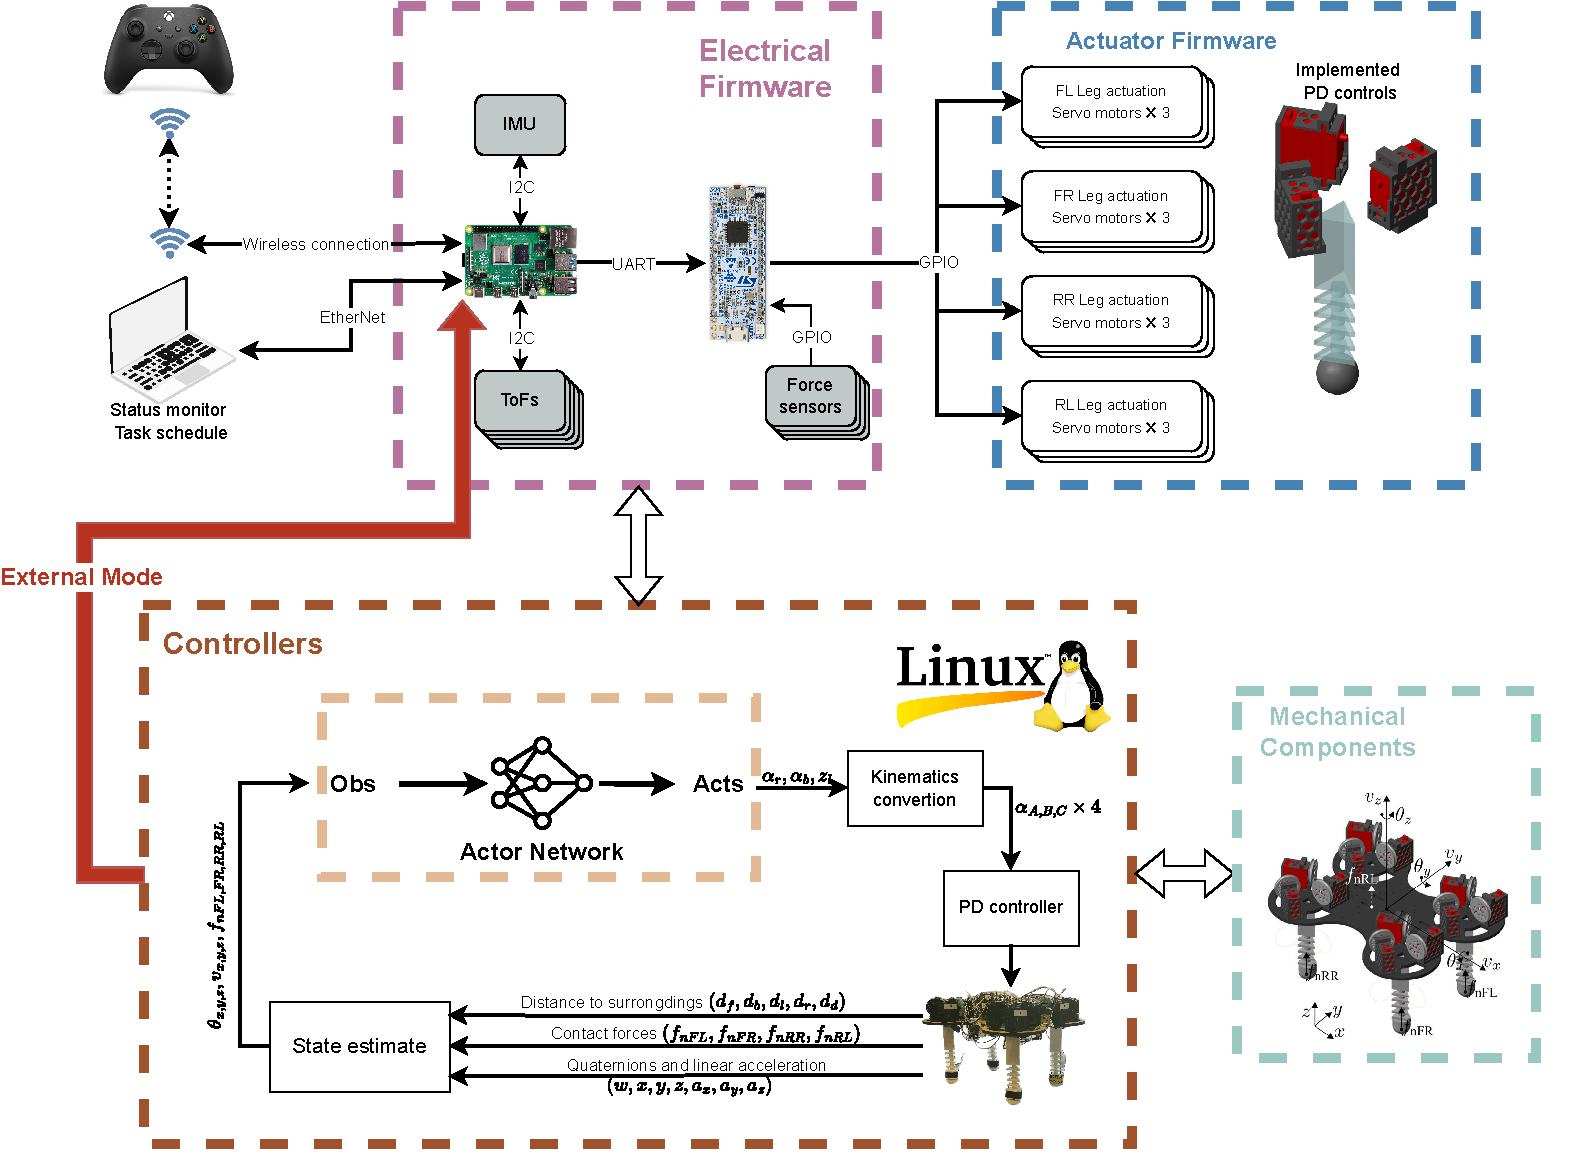
\includegraphics[width=\linewidth]{img/chap4/control.pdf}
    \caption{Graphical overview of control architecture of SoftQ.}
    \label{fig:control}
\end{figure}

The locomotion of SoftQ is profoundly governed by servo motors, which receive \ac{PWM} signals from the STM32 microcontroller. These signals translate into specific rotational torques applied to the actuators, leading to controlled limb motions for different gaits. The servo motors feature built-in position controllers that respond to PWM signals, ensuring precise motor positioning.

The STM32 microcontroller manages contact forces and controls the servo motors through \ac{GPIO} pins. It efficiently processes commands from the Raspberry Pi, generating PWM signals in response to Simulink controller commands. This fine-grained control guarantees accurate execution of the robot's intended actions. Additionally, the STM32 interfaces with force sensors, reading voltage values across them. These voltage changes help the controller determine the applied forces' magnitude, serving as feedback for the robot to adapt its movements to external forces. Communication between the Raspberry Pi and STM32 utilizes \ac{UART} for command and data exchange.

The Raspberry Pi directly interfaces with a variety of sensors and devices to gather supplementary information for guiding the robot's control. These vital observations encompass quaternion angles, linear accelerations, and distance data, all of which are acquired through the \ac{I²C} interface. The quaternion angles, originating from the \ac{IMU}, provide a representation of the robot's orientation in three-dimensional space. For a detailed description of the conversion process from quaternion to Euler angles, please refer to Section \ref{sec:Q2E}. To enhance the situational awareness, these quaternion angles are converted into Euler angles, specifically roll, pitch, and yaw. The IMU itself is a sophisticated 9-DOF sensor, featuring integrated sensor fusion capabilities via its onboard microcontroller. This functionality allows the IMU to provide additional fused data, including linear accelerations in three axis. The linear accelerations is subsequently integrated with distance data from \ac{ToF} sensors to estimate the robot's actual velocity. ToF sensors employ the time-of-flight principle by emitting light pulses that bounce off objects, returning to the sensor to calculate the mean distance within a square area in front of it, measuring the distance between the sensor and the reflecting object.

In the context described, the Simulink controller plays a crucial role by assuming the task of generating the robot's actions through external mode operation on the Raspberry Pi. This entails the generation of control commands, which are determined based on the assessment of states inferred from direct observations. To facilitate this process, raw data such as orientation, linear accelerations, and contact forces of the robot are subjected to preprocessing, transforming them into states ($\mathbf{s}_t$) that can serve as inputs for the actor network. The actor network, which is derived from a converged SAC algorithm, serves as the core component in this control scheme. The actor network takes on the critical task of planning an optimal gait, generating actions that enable the robot to move forward effectively. However, it is essential to note that these actions, produced by the actor network, must undergo a further transformation before they can be effectively utilized by the lower-level controllers. This transformation step involves the conversion of the actions into motor commands. This conversion process relies on inverse kinematic relations, as outlined in Equation \ref{eq:value2motor}. This ensures that the actions generated by the actor network are translated into commands that directly influence the robot's motors, thereby enabling the desired movements and control of the robot's behavior.

Furthermore, the Raspberry Pi establishes wireless communication with a PC to enhance its functionality. The PC serves as a conduit for transferring MATLAB Simulink programs to the Raspberry Pi via external mode. It also acts as a Graphical User Interface (GUI), enabling seamless human-robot interaction. The GUI offers real-time status updates, providing immediate insights into the robot's performance and operation. Moreover, it facilitates the reception of tasks and instructions from the operator, allowing real-time directive issuance. This bidirectional communication between the PC and the robot enhances versatility and adaptability. Additionally, the control system accommodates user input, offering various interfaces like joysticks or command line velocity inputs for real-time robot guidance and adjustments.

\subsection{Task Planning and Execution}
The control architecture of the soft quadruped robot encompasses a multifaceted orchestration of task planning and execution, which plays a pivotal role in the robot's ability to achieve its goals with precision and adaptability. This section delves into the specific architecture of task planning and execution at software side within the control framework. 

The core of the robot's control architecture is centered around the efficient utilization of multi-threading. Each thread is responsible for a specific aspect of the robot's operation, and these threads run concurrently, allowing for parallel processing and efficient resource management. This concurrent execution is particularly advantageous in enhancing the robot's ability to perform multiple tasks simultaneously. Notably, the Raspberry Pi serves as the primary processing unit responsible for coordinating the robot's actions. Within this Raspberry Pi-based control unit, four distinct threads operate in unison to orchestrate the robot's functions: 
\begin{itemize}
    \item UDP\_Transmit Thread (20 Hz): This thread is responsible for reading, composing and transmitting observational data to the Simulink environment via User Datagram Protocol (UDP). It facilitates the seamless exchange of sensory information gathered by the robot with the Simulink simulation. The frequency is bounded by the I²C communication of 5 ToFs. 
    \item UDP\_Receive Thread (50 Hz): The UDP\_Receive thread specializes in receiving motor control commands from the Simulink environment via UDP communication. It ensures that the robot can receive real-time instructions from the simulation, allowing for dynamic control adjustments. Importantly, this thread operates conditionally, only receiving commands when a specific counter condition is met, contributing to safety and controlled execution.
    \item com2STM32 Thread (20 Hz): This thread is responsible for bidirectional communication with the STM32 microcontroller, which interfaces with the robot's hardware components. It sends relevant control data to the STM32 unit, enabling the robot to perform physical actions. Simultaneously, it receives sensor readings and feedback from the STM32, providing crucial information about the robot's state and surroundings. The frequency is bounded by the computation load from Simulink. 
    \item Countdown Thread (0.5 Hz): The Internal Countdown thread operates at a lower frequency of 0.5 Hz. Its primary role is to manage a countdown mechanism that regulates the activation of flags to the STM32, indicating when motor commands received from Simulink can be executed.
\end{itemize}

One fundamental aspect of this architecture is its decentralized nature. Instead of relying on a single central controller, the robot employs a distributed control strategy. Each thread is designed to handle a specific subset of tasks or functionalities. For instance, the STM32 process operates on an event-triggered basis, only executing motor commands when received from the Raspberry Pi. It also sends back contact force readings, adding a feedback loop to the control process. Additionally, the presence of flags controlling the switch of power sources ensures that only reliable motor commands obtained from Simulink are executed, further enhancing the safety and reliability of the robot's actions. 
\begin{figure}[htb]
    \centering
    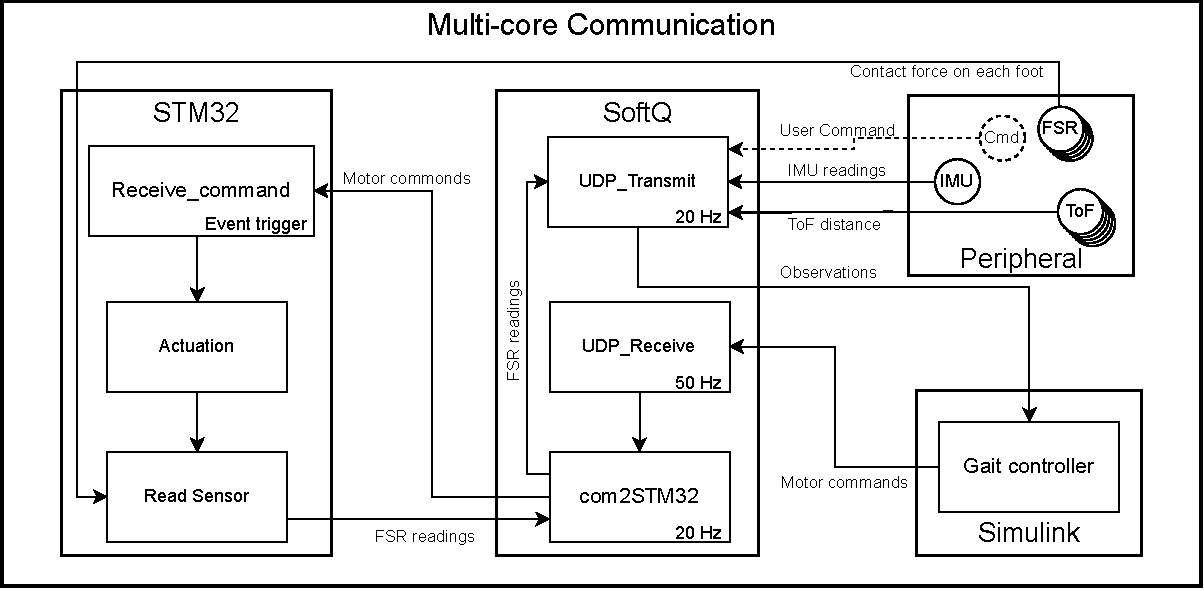
\includegraphics[width=0.9\linewidth]{img/chap4/process.pdf}
    \caption{Schematics of multi-core communication of SoftQ.}
    \label{fig:process}
\end{figure}

To facilitate cooperation among these threads and processes, a well-defined mechanism for multi-core communication and data sharing is established. This mechanism allows threads to exchange information and synchronize their actions. The schematic representation of this multi-core communication is illustrated in Figure \ref{fig:process}. To exemplify this inter-thread communication, consider the SoftQ process running on the Raspberry Pi. Within this context, a "Thread-Safe Data Access" mechanism is meticulously implemented. This involves encapsulating shared data within a dataclass, a structured approach that helps prevent data corruption or conflicts in a multi-threaded environment. Furthermore, synchronization mechanisms such as locks or semaphores are judiciously employed. These synchronization tools serve as safeguards, ensuring that only one thread can access and modify shared data at any given time, thus mitigating the risk of data inconsistency or errors. In addition, the control architecture benefits from pre-designed Direct Memory Access (DMA) and Interrupts Muralidharan et al.\cite{thorapallimuralidharanContinuumActuatorBased2020} and Danelia et al.\cite{daneliaStructureGaitOptimizationof2021}. These advanced techniques enhance data transfer efficiency and response times, further augmenting the control system's capabilities.

\subsection{Sensor Fusion by Kalman Filter}
In this section, the focus shifts to the implementation of a Kalman filter for sensor fusion, a critical element of the research aimed at acquiring precise velocity information. The quest for accurate velocity data is driven by the core objective of achieving precise control and adaptability in the deployment of MBRL on physical robots. Velocity estimation is approached by differentiating the position component over time, with particular attention given to forward walking scenarios, where the angular velocity component can be safely disregarded. The instant velocity calculated based on the distance data from the ToF sensors is plotted in Figure \ref{fig:KF}. However, this velocity exhibits a sharp changes and may not effectively capture dynamic changes in velocity. Furthermore, the computed velocity may result from the integration of linear acceleration over time, as plotted in Figure \ref{fig:KF}. This approach, unfortunately, is susceptible to inaccuracies, with the calculated velocity exhibiting constant fluctuations even in the absence of motion. The source of this inaccuracy is attributed to the drift present in the acceleration data acquired from the IMU. Consequently, the velocity estimation from acceleration reaches a constant value at -0.8 m/s after walk. 
\begin{figure}[htb]
    \centering
    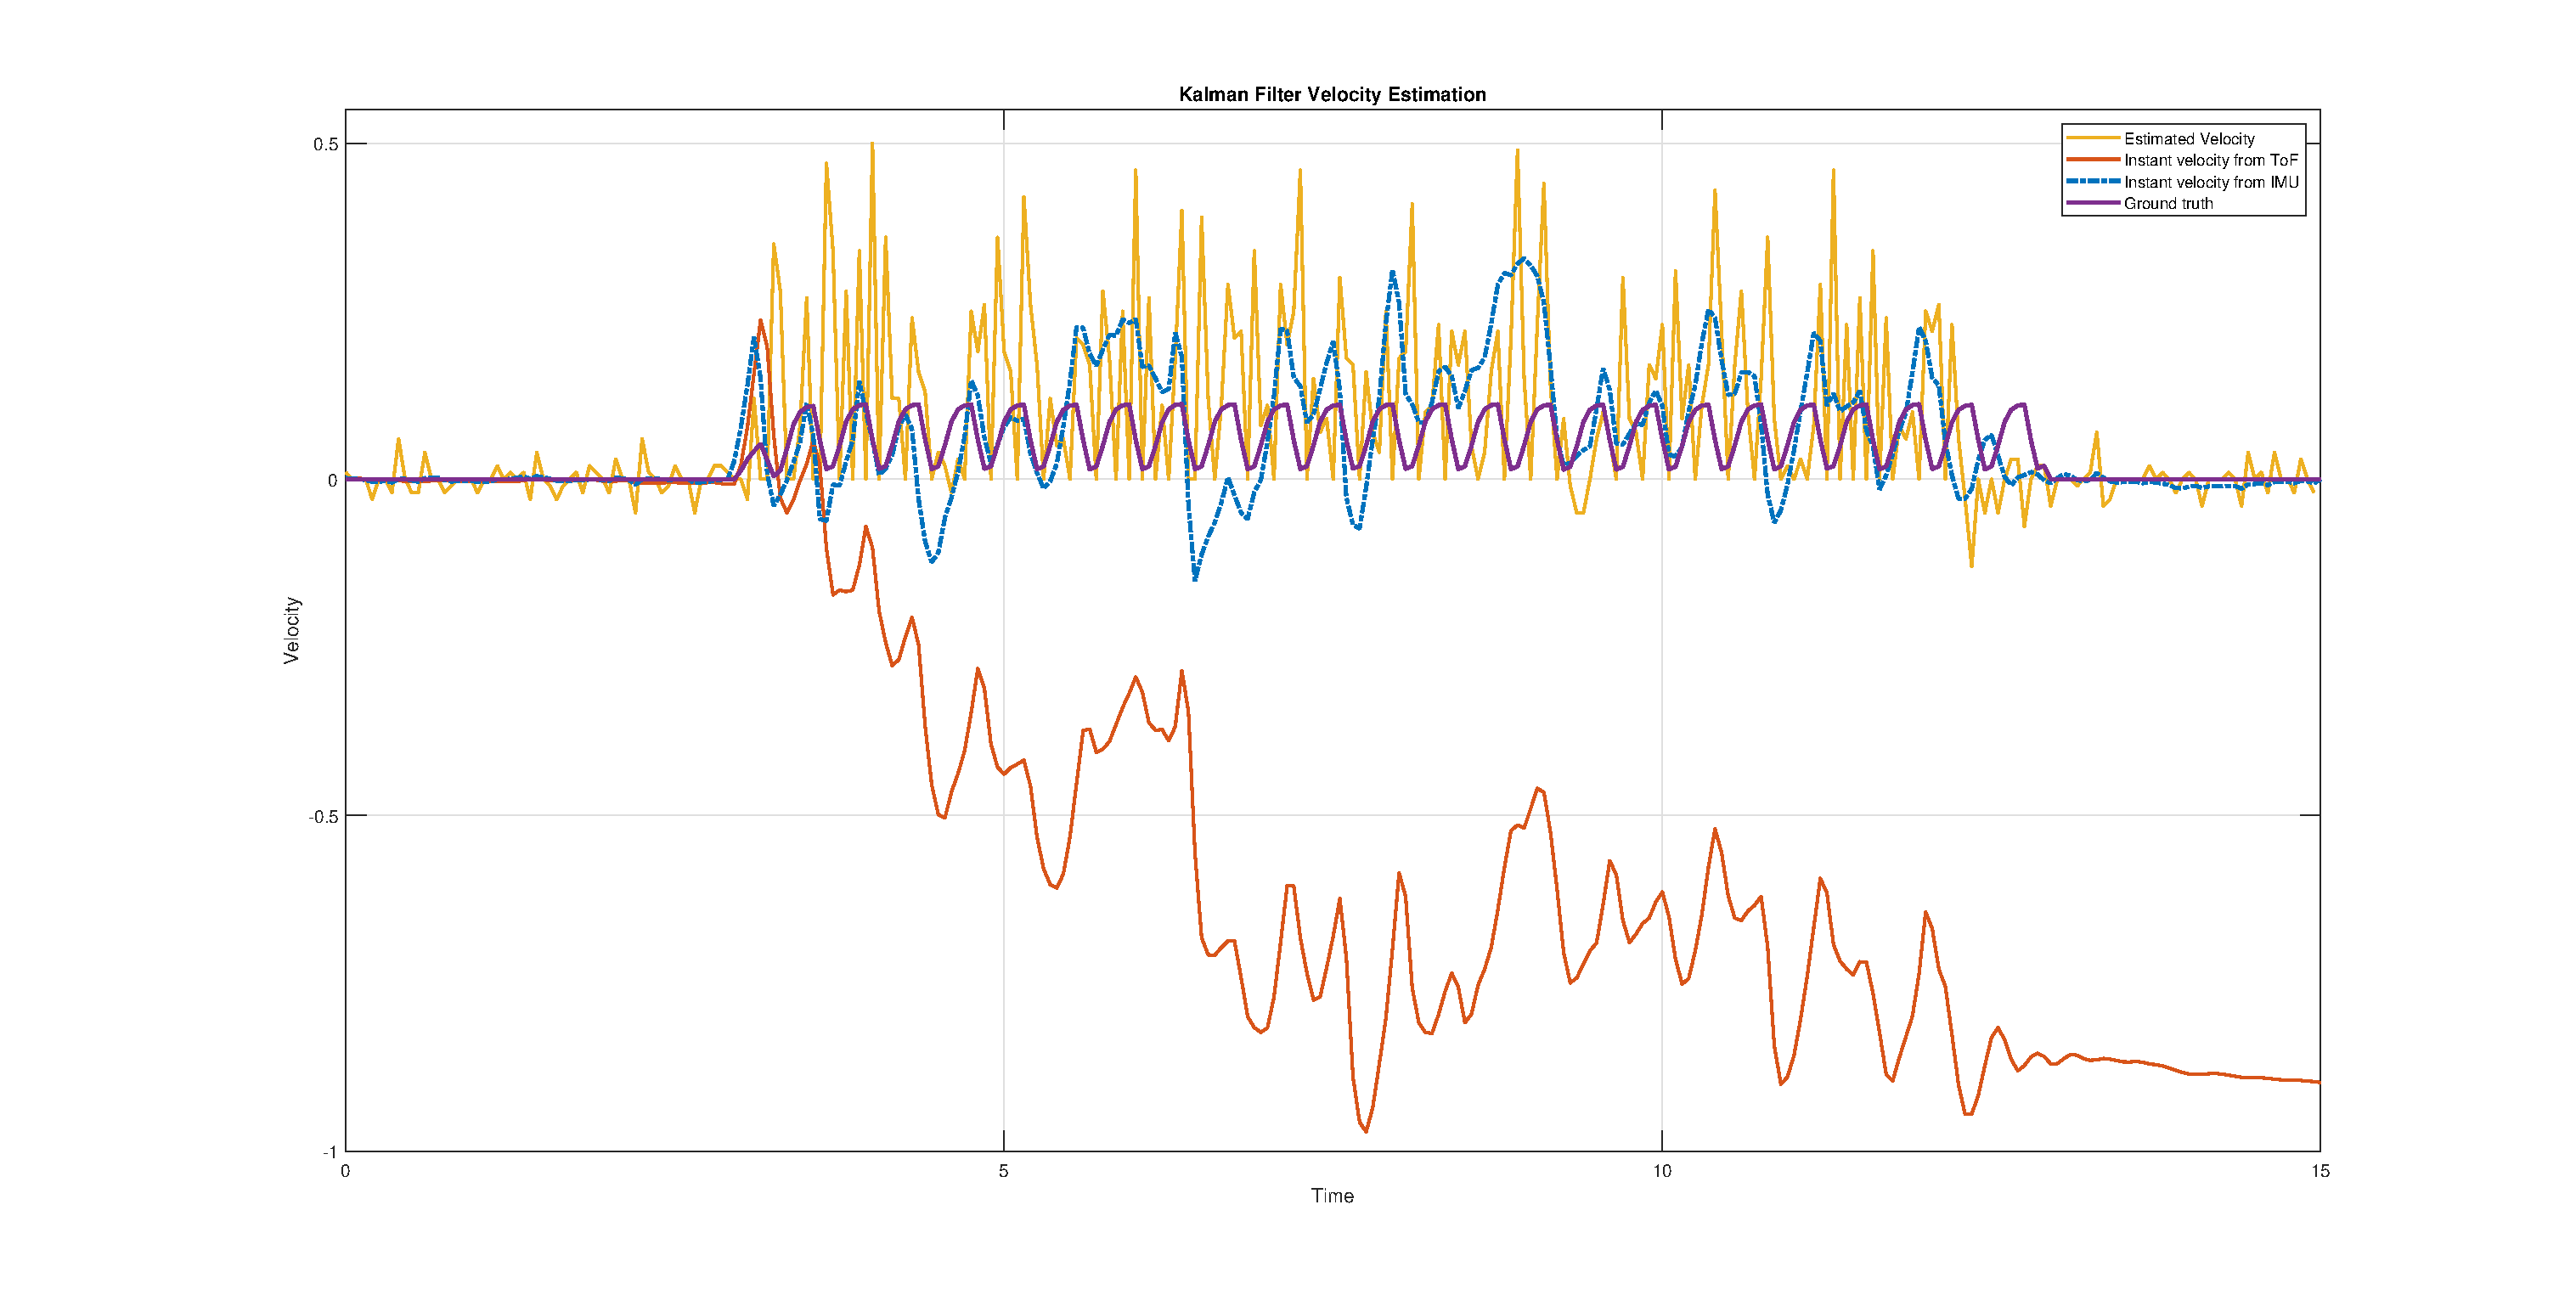
\includegraphics[width=\linewidth]{img/chap4/KF.eps}
    \caption{Velocity estimation in x-axis ($v_x$) through Kalman filtering of ToF and IMU data.}
    \label{fig:KF}
\end{figure}

To achieve a more accurate and precise velocity estimation, a Kalman filter has been specifically designed and integrated into the control architecture. The Kalman filter assumes a crucial role in reducing sensor electronic noise, addressing measurement inaccuracies, mitigating sensor noise, and minimizing quantization errors when predicting velocity from acceleration and position measurements. However, it is important to note that obtaining ground truth velocity data from the real robot is complex. Therefore, we used velocity data from simulations of the tested expert gait as a reference, as shown in Figure \ref{fig:KF}. The Kalman filter's estimation appears to capture most of the movement periods, although some inconsistencies remain. This is attributed to the reality gap, as the robot faces challenges in maintaining a relatively constant speed due to differences in ground conditions and other factors in the real-world environment.

Kalman filter is a linear optimal states estimation method, which is known as one of the most famous Bayesian filter theories. State equation is a linear representation of a state vector $x_{k-1}$, a process noise matrix $w_{k}$ and a control input vector $u_{k}$. Observation equation is a linear representation of a state vector $x_{k}$ and a measurement noise vector $v_{k}$. A dynamic model is presented with state equation and observation equation through the reliable estimation corrected by measurements, which is shown in Equation \ref{eq:kf}.

\begin{equation}
    \begin{aligned}
        \text{State Equation:} \quad & x_{k} = A x_{k-1} + B u_{k-1} + w_{k} \\
        \text{Observation Equation:} \quad & z_{k} = H x_{k} + \nu_{k}
    \end{aligned}
\label{eq:kf}
\end{equation}

In the above formulas: $A$, $H$, $w_{k}$, $\nu_{k}$ is the state transition matrix, the observation matrix, the system noise vector, the observation noise vector, respectively. $w_{k}$ and $\nu_{k}$ are assumed to satisfy positive definite, symmetric and uncorrelated, zero mean Gaussian white noise vector. $w_{k}$ is a random variable with a multivariate normal distribution, where the covariance matrix is $Q$. $\nu_{k}$ is also assumed to be a random variable with a multivariate normal distribution, where the covariance matrix is $R$. In addition, The state covariance matrix, denoted as $P$, is a symmetric matrix that provides information about the uncertainty in the state variables being estimated by the Kalman filter. $P$ undergoes continuous updates as the Kalman filter processes new measurements and predictions. In specific, the Kalman filter is appled to a linear system, and the system dynamics can be approximated as a linear relation between the acceleration $a$, velocity$v$ and position $p$, namely 
\begin{align*}
    \begin{cases} 
    p = p + T_s\cdot v + \frac{T_s^2}{2}\cdot a\\
    v = v + T_s\cdot a
    \end{cases}
    \label{eq:kf_dynamics}
\end{align*}

Defining the states as $x_1 = p$, $x_2 = v$ and the input $u = a$, the model could be transformed into state space form
\begin{equation}
    \begin{cases} 
    \mathbf{x}_{k+1} = \begin{bmatrix}p \\v \end{bmatrix} = \underbrace{\begin{bmatrix}1 & T_s \\0 & 1\end{bmatrix}}_{A} \mathbf{x}_k + \underbrace{\begin{bmatrix}\frac{T_s^2}{2}  \\T_s \end{bmatrix}}_{B} u_k \\
    y_k = \underbrace{\begin{bmatrix}1\;0\end{bmatrix}}_{H} \mathbf{x}_k
    \end{cases}
    \label{eq:kf_state}
\end{equation}

The Kalman gain $K$ determines the weight given to incoming measurement data when updating the estimated state of a dynamic system. In each step, $K_k$ is updated by $P_k$, $K_k=\frac{P_kH}{HP_kH^T+R}$. The Kalman gain $K_k$ emerges as a critical factor in adjusting the state estimate in response to incoming measurements, as outlined in the state estimation equation:
\begin{equation}
    \hat{\mathbf{x}}_{k+1} = A\hat{\mathbf{x}}_{k-1} + Bu_k + K_k\cdot(z_k - H\hat{\mathbf{x}}_{k-1})
    \label{eq:kf_est}
\end{equation} 
In this equations, $\hat{\mathbf{x}}_{k+1}$ is the updated state estimate, $u_k$ is the control input, $z_k$ is the measurement in position. The observer is interpreted as a one-step predictor, which forecasts the system states at the next time instance $k+1$ by utilizing the estimated states at time $k$, along with additional feedback from the estimation error, weighted by the Kalman gains. Since the disturbance primarily affects the acceleration, we can update the structure of $Q$ accordingly. The process noise covariance matrix $Q$ should reflect the covariance of disturbances in acceleration ($\sigma_a^2$) and how they propagate through the system. In a simplified form, it might look like: $Q = \begin{bmatrix}0.01 & 0 \\0 & 1\end{bmatrix}$, and the observation noise covariance matrix is set as $R = 0.15$. Additionally, the observation noise covariance matrix is tuned to be $R = 0.1$, and initial state estimates ($\mathbf{x}_0$) and initial error covariance estimates ($P_0$) are provided as: $\mathbf{x}_0 = \begin{bmatrix} 0 \\ 0 \end{bmatrix}$ and $P_0 = \begin{bmatrix}1 & 0 \\0 & 1\end{bmatrix}$. 

The detailed process of how the Kalman filter is updated and applied can be found in Section \ref{sec:kf}. Before incorporating sensor measurements into the Kalman filter, a preprocessing step was performed to bound and average the measurements, ensuring their reliability and stability. The same Kalman filter for sensor fusion was employed for velocity estimation in both the $x$ and $y$ axes. This choice was driven by the presence of two Time-of-Flight (ToF) sensors dedicated to these axes. Conversely, in the $z$ axis, which represents vertical motion, a single ToF sensor located at the bottom was used. The optimal state observer, known as the Kalman filter provides the optimal estimate of $\mathbf{x}$ minimizing the covariance matrix $P$ of the estimation error $\hat{\mathbf{x}}$ using series of noisy measurements. As the Kalman filter iteratively processed sensor measurements, it progressively refined its estimates of velocity. The results of velocity estimation, facilitated by the Kalman filter application, are visualized and presented in Figure \ref{fig:KF}. These plots provide a clear representation of the refined velocity estimates and underscore the effectiveness of the Kalman filter in mitigating sensor noise and enhancing the overall reliability of the velocity sensing.

\section{Potential Reality Gap}
Transitioning to a different facet of consideration, it is crucial to address the concept of the "Potential Reality Gap." In the realm of reinforcement learning, the surrogate model serves as a bridge between simulation environments and real-world scenarios. However, due to the inherent complexity and uncertainty associated with real-world environments, a misalignment often arises between the training data collected from simulations and the actual performance of the trained model in real-world situations. This discrepancy is referred to as the "Reality Gap."

The Reality Gap poses a challenge because the surrogate model might perform exceptionally well during training in simulation environments but struggle to generalize effectively to real-world settings. This phenomenon can be attributed to various factors, including disparities in physical dynamics, sensor noise, and unmodeled environmental influences. To address the Reality Gap, certain strategies can be adopted. One approach involves introducing stochasticity during training in simulations, simulating uncertainties and disturbances that are characteristic of real-world scenarios, where zero mean Gaussian noise is introduced into all observation signals. This additional noise is independently sampled from zero-mean Gaussian distributions in a random manner. Based on the sensor calibration results, the variances of the noise applied to the velocity, angular and force signal data are set to: $\sigma_{\pmb{\theta}}^2 = 0.002$, $\sigma_{\mathbf{v}}^2 = 0.002$ and $\sigma_{\mathbf{f}_n}^2 = 0.005$, respectively. By incorporating such noise into the training process, the model is better equipped to develop robustness and adaptability, allowing it to effectively handle unexpected variations and challenges encountered in real-world applications.

In an effort to mitigate the Reality Gap, it is worth noting that the SAC algorithm offers commendable exploration capabilities. This presents the opportunity to retrain a converged agent with the potential to adapt its policy for various tasks. Consequently, the converged policy guiding the robot's walking behavior, as determined by MBRL, can be repurposed as the initial policy for continued training with a more accurate model, facilitating the reduction of the Reality Gap, which is so-called continuous training.

The continuous training begins by extracting the policy that has been converged during the initial MBRL training. This policy is the result of the agent's learning process and encapsulates the knowledge it has gained about optimal gait control. To address the reality gap, the converged policy is integrated with a more accurate simulation model in Matlab. This simulation would strive to closely replicate the real-world dynamics and physics of the robot. The use of a more accurate model helps in reducing the discrepancies between simulation and reality. The training process begins with the converged policy as the starting point. This initial policy is influenced by the agent's prior learning, facilitating faster adaptation to the refined simulation environment. Depending on the specific goals and challenges of the new simulation setup, it is important to adjust the reward structure by fine-tuning reward functions to align with desired behavior or objectives in the updated environment. Once the continuous training process has yielded a sufficiently adapted policy, this policy can be transferred to the physical robot for real-world testing. 
\chapter{Results}
\label{chap5}
\textit{This chapter presents the results of the experiments and evaluations conducted in this research. It provides a detailed analysis of the performance of MBRL algorithms with continue training and provide insights into the research questions posed at the beginning of this study.}

\section{Surrogate Model Performance}
\subsection{Performance Evaluation}
To evaluate the surrogate model's performance, it is important to consider several critical metrics. These metrics serve as crucial indicators of how effectively the model approximates and forecasts the robot's behavior. Here, these metrics are elaborated without delving into details:
\begin{itemize}
    \item Average Steps before Failure: This metric assesses the model's capacity to predict the duration of a simulation run without encountering failure, serving as an indicator of sample efficiency.
    \item Validation RMSE and Validation Loss: This RMSE quantifies the disparity between the surrogate model's predictions and the actual values present in the validation dataset, as defined in Equation \ref{eq:RMSE}. Lower RMSE values are indicative of a higher degree of precision and accuracy in forecasting future states ($s_{t+1}$). Concurrently, the Validation Loss serves as an overarching measure of the model's performance on the validation dataset, underscoring the significance of minimizing this metric to enhance predictive capabilities, as defined in Equation \ref{eq:loss}.
    \item NRMSE: NRMSE provides a normalized measure of error, enabling comparisons of prediction accuracy across expert pattern datasets. It proves particularly valuable in evaluating the surrogate model's ability to predict sensor observations on the robot. The single step prediction NRMSE is calculated by Equation \ref{eq:NRMSE}, the long-term prediction NRMSE is calculated by Equation \ref{eq:NRMSET}.
    \item Correlation Coefficient (R): The R quantifies the linear relationship between simulated and predicted values, as specified in Equation \ref{eq:R}. A higher R signifies a more robust correlation, highlighting the model's proficiency in capturing underlying data trends and patterns.
\end{itemize}

\subsection{Control Variables Restriction}
The investigation commences with a focused exploration of state-space restriction within the surrogate model. The state-space, encompassing both observations and actions, is defined as $\mathbf{s}_t = [\pmb{\theta}(t), \mathbf{v}(t), \mathbf{f}n(t), \mathbf{a}_{t-1}]$ in Section \ref{sec:ss}. It is worth noting that the first three terms in this state-space originate from observations and are inherently challenging to restrict, but the action space can be subject to constraints.  It's crucial to acknowledge that the first three terms in this state-space comes from observations and present inherent challenges for restriction, but the action space can indeed be subjected to constraints. 

An important aspect to underscore is that the restriction of the robot's action space was achieved through the application of pattern-defined modeling techniques. Specifically, the robot's legs are interconnected in diagonal pairs, similar to a trotting pattern. This inherent structural arrangement significantly simplifies the action space compared to dealing with the complexity of controlling 12 individual motor actions\cite{jiSynthesizingOptimalGait2022}, effectively reducing it from $\mathbf{a}\in\mathbb{R}^{12}$ to $\mathbf{a}\in\mathbb{R}^4$. 

Furthermore, an alternate method of parameterization was applied, where the surrogate model's configuration incorporates specific control variables. Within this context, the actions are as defined in Section \ref{Sec:as}, taking the form of $\mathbf{a}_{t} = [\alpha_{b_1}, z_{l_1},\alpha_{b_2},z_{l_2}]$. These variables are subject to the bounds governed by the gains ($\alpha_{b_{gain}}\, , z_{l_{gain}}$). It's also crucial to emphasize that these gains associated with actions hold significance not only in the construction of the surrogate model but also play a vital role in shaping the behavior and adaptability of the SoftQ. Therefore, our focus centers on two key components within the action space: the gain of bending angle $\alpha_{b_{gain}}$ and the gain of compression length $z_{l_{gain}}$ for each of the diagonal leg pairs. To address this aspect, a series of simulations involving random actions within a bounded action space were carried out. These simulations aimed to gather the necessary data required for training the surrogate model. Subsequently, the performance of the trained model was evaluated. To effectively assess the trained neural networks performance, a color heat map can be employed to provide a visual representation of various performance metrics, as shown in Figure \ref{fig:NN_heat}. Each metric is associated with a specific color scale, allowing for a quick and intuitive evaluation.

\begin{figure}[htb]
    \centering
    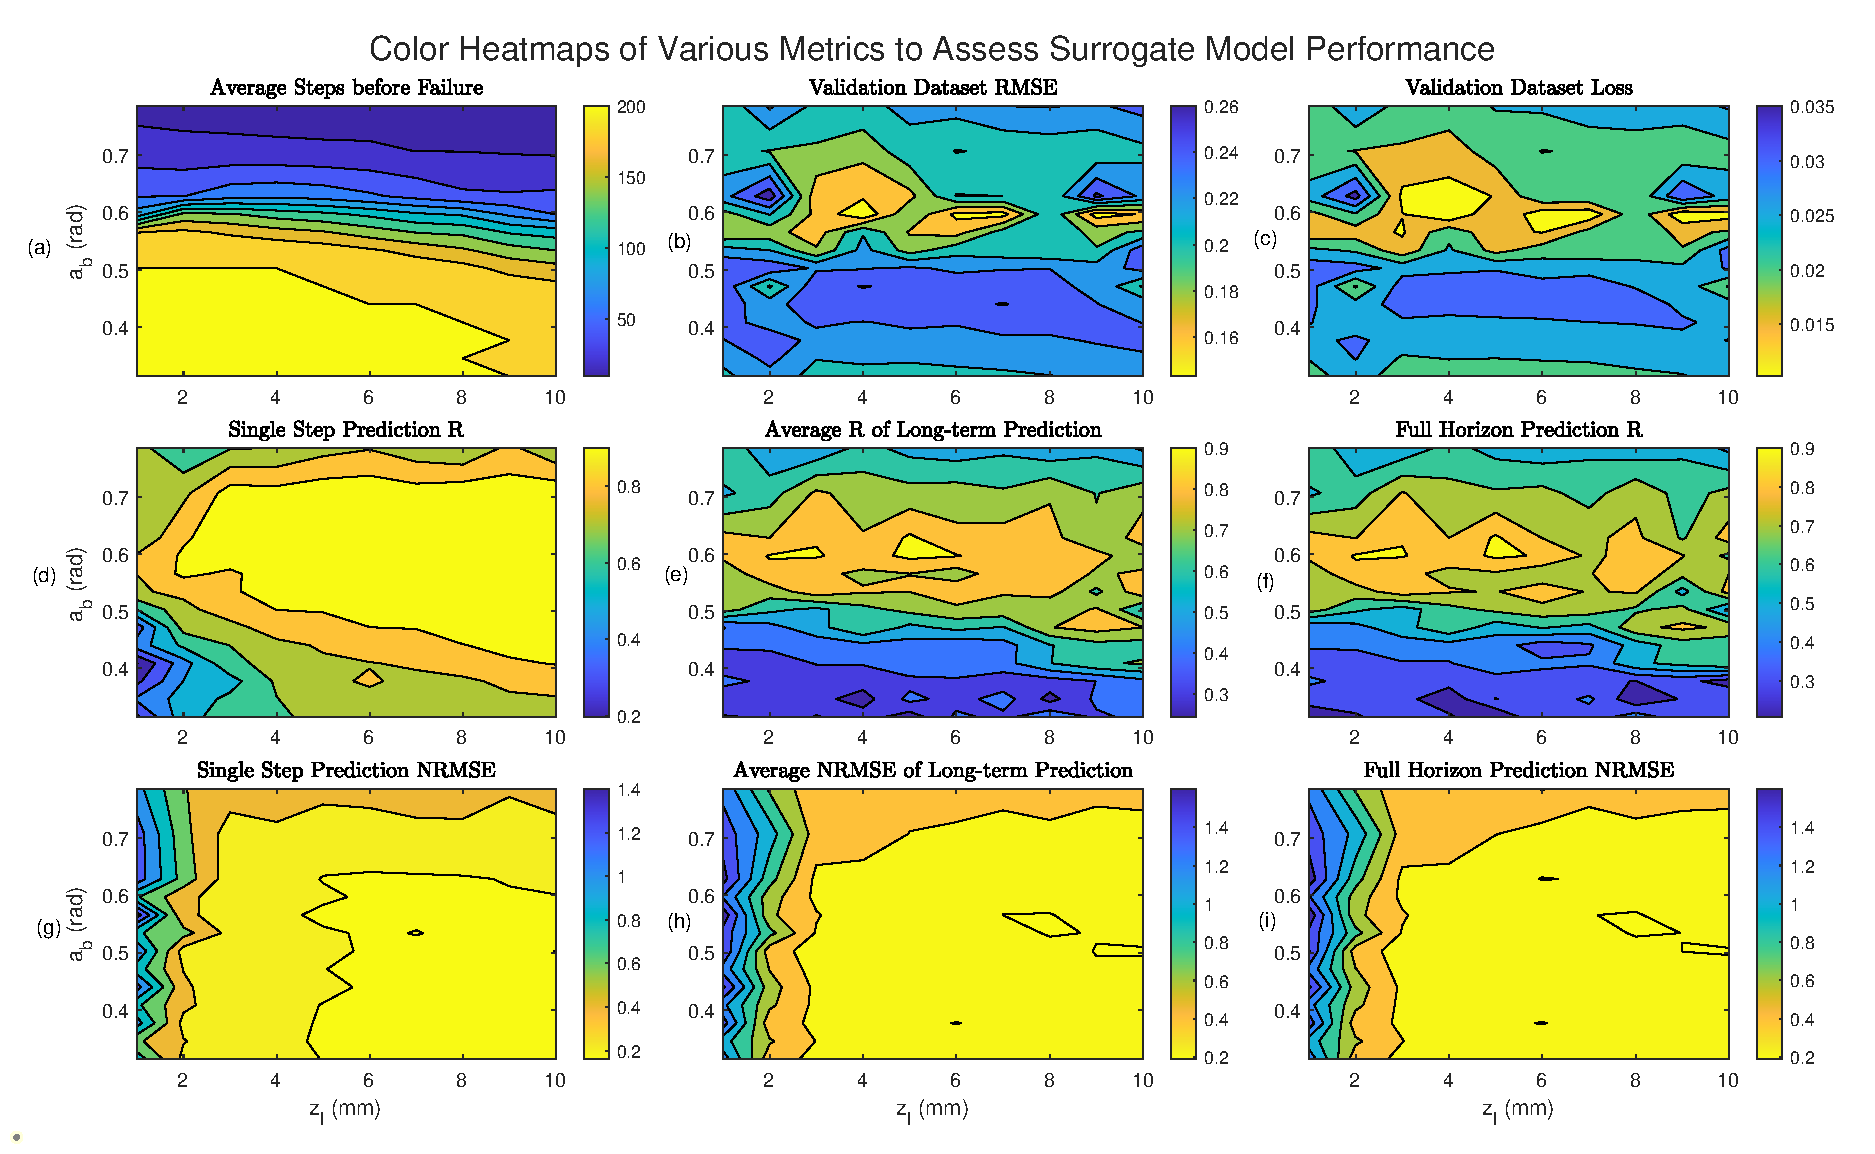
\includegraphics[width=\linewidth]{img/chap5/NN_heat.eps}
    \caption{Visualization of Performance Metrics Through Color Heat Map for Evaluating Trained Surrogate Models. The metrics include: (a) Average Steps before Failure; (b) \ac{RMSE} on the Validation Dataset; (c) Loss on the Validation Dataset; (d) Single Step Prediction Coefficient R; (e) Average Coefficient R for Long-term Prediction; (f) Coefficient R for Full Horizon Prediction; (g) NRMSE for Single Step Prediction; (h) Average NRMSE for Long-term Prediction; (i) NRMSE for Full Horizon Prediction.}
    \label{fig:NN_heat}
\end{figure}

In Figure \ref{fig:NN_heat}(a), it is evident that reducing the lower restrictions within the action space leads to an increase in the average number of steps the system can take before encountering failure, indicating improved data efficiency due to reduced locomotion risk with smaller actions. In Figure \ref{fig:NN_heat}(c), all neural networks converge with a loss below 0.037 in the validation dataset, with minimal differences between them. In Figure \ref{fig:NN_heat}(b), validated in the same dataset, RMSE converges to a minimum level. Notably, better validation RMSE is achieved when $\alpha_b$ ranges from 0.55 to 0.7 radians and $z_l$ ranges from 3 to 9 millimeters, suggesting optimal model performance within these parameter ranges.

In assessing single-step predictions using various expert gait pattern datasets, the correlation coefficient (R) between predictions and ground truth was calculated, as depicted in Figure \ref{fig:NN_heat}(d). The results show consistently high accuracy when either the compression length ($z_l$) or the bending angle ($\alpha_b$) is high, or when both are elevated. This observation aligns with the expectation that for the robot to achieve higher speeds, it should exhibit more pronounced behaviors, which are characterized by larger values of these parameters. Consequently, the expert gait dataset used in this context emphasizes high values of $\alpha_b$ and $z_l$, resulting in smaller differences between predictions and ground truth, and consequently, lower values of R. A similar trend is observed when considering single-step predictions. Smaller NRMSE values are associated with high values of $z_l$ and $\alpha_b$, but interestingly, low $\alpha_b$ values also yield small NRMSE values. This implys that bending angle ($\alpha_b$) exerts a more significant influence on robot locomotion. These results are visually represented in Figure \ref{fig:NN_heat}(g). However, it is important to note that neither the NRMSE nor R reach their lowest points in the highest $\alpha_b$ region, suggesting poorer predictions when too small steps are taken before simulation failure, resulting in an insufficient amount of useful data.

For multi-step predictions on the same expert gait pattern datasets, the effects of $\alpha_b$ and $z_l$ are similar in single step prediction, but the models with low $\alpha_b$ values perform less effectively in predicting over longer time horizons, suggesting a lack of robust generality in these models. However, as shown in Figure \ref{fig:NN_heat}(e), the average correlation coefficient (R) for long-term predictions reveals that models with relatively high values of both $\alpha_b$ and $z_l$ struggle to predict states over extended horizons. This challenge could be attributed to the larger action space, which introduces more unpredictability and subsequently leads to reduced performance compared to models with lower $z_l$ values when trained on the same dataset size. This trend is also evident in the full horizon prediction R, as depicted in Figure \ref{fig:NN_heat}(f), where predictions at relatively high values of both $\alpha_b$ and $z_l$ deteriorate. In addition, the average NRMSE of long-term predictions exhibits a similar performance to what was observed in single-step predictions, which shows different patterns compared to R results, because the NMRMSE is normalised and large values like contact forces may have more effects on the metrics. Lower errors are associated with larger values of $\alpha_b$ and $z_l$, but NRMSE also decreases when $\alpha_b$ reaches its highest values. These results are presented in Figure \ref{fig:NN_heat}(h). Interestingly, performance remains consistent when $\alpha_b$ is smaller than 0.72 radians and $z_l$ is larger than 3 millimeters. Likewise, in the case of NRMSE for full horizon prediction, there is no significant change in performance, as indicated in Figure \ref{fig:NN_heat}(i).

Hence, the optimal action state restrictions can be identified as approximately $\alpha_b$ around 0.6 rad and $z_l$ around 7 mm. However, it's important to consider that these restrictions also impact MBRL training, as they limit the range of exploration within the robot's action space. Therefore, it's preferable to keep the action space as broad as possible. Another viable set of restrictions to consider is $\alpha_b$ around 0.63 rad and $z_l$ around 8 mm for the state space during surrogate model training and MBRL training. This broader range allows for more exploration and potentially better overall performance in subsequent MBRL learning.

\section{Model-based RL Training}
After the surrogate model determined in Section \ref{sec:NN_design}, we can continue to training of MBRL for optimal gait controls, which will be used as a gait controller in robot to navigate with learned optimal gait. It's important to note that the training settings remained consistent across all experiments. The code snippet for training details can be found in Section \ref{code:mbrl}. To account for potential variations due to randomness, the training process was initiated with various random seeds. It was observed that training had a higher failure rate when the agent became trapped in local minima. Consequently, it can be intuitively inferred that mastering the policy for low-speed locomotion posed a more challenging task for the agent. Notably, in the experiments, $v_{ref}$ was maintained at no smaller than 0.1 m/s to ensure meaningful training outcomes and the final time of the training in one episode $T_f$ is 10 seconds.
\begin{figure}[htb]
    \centering
    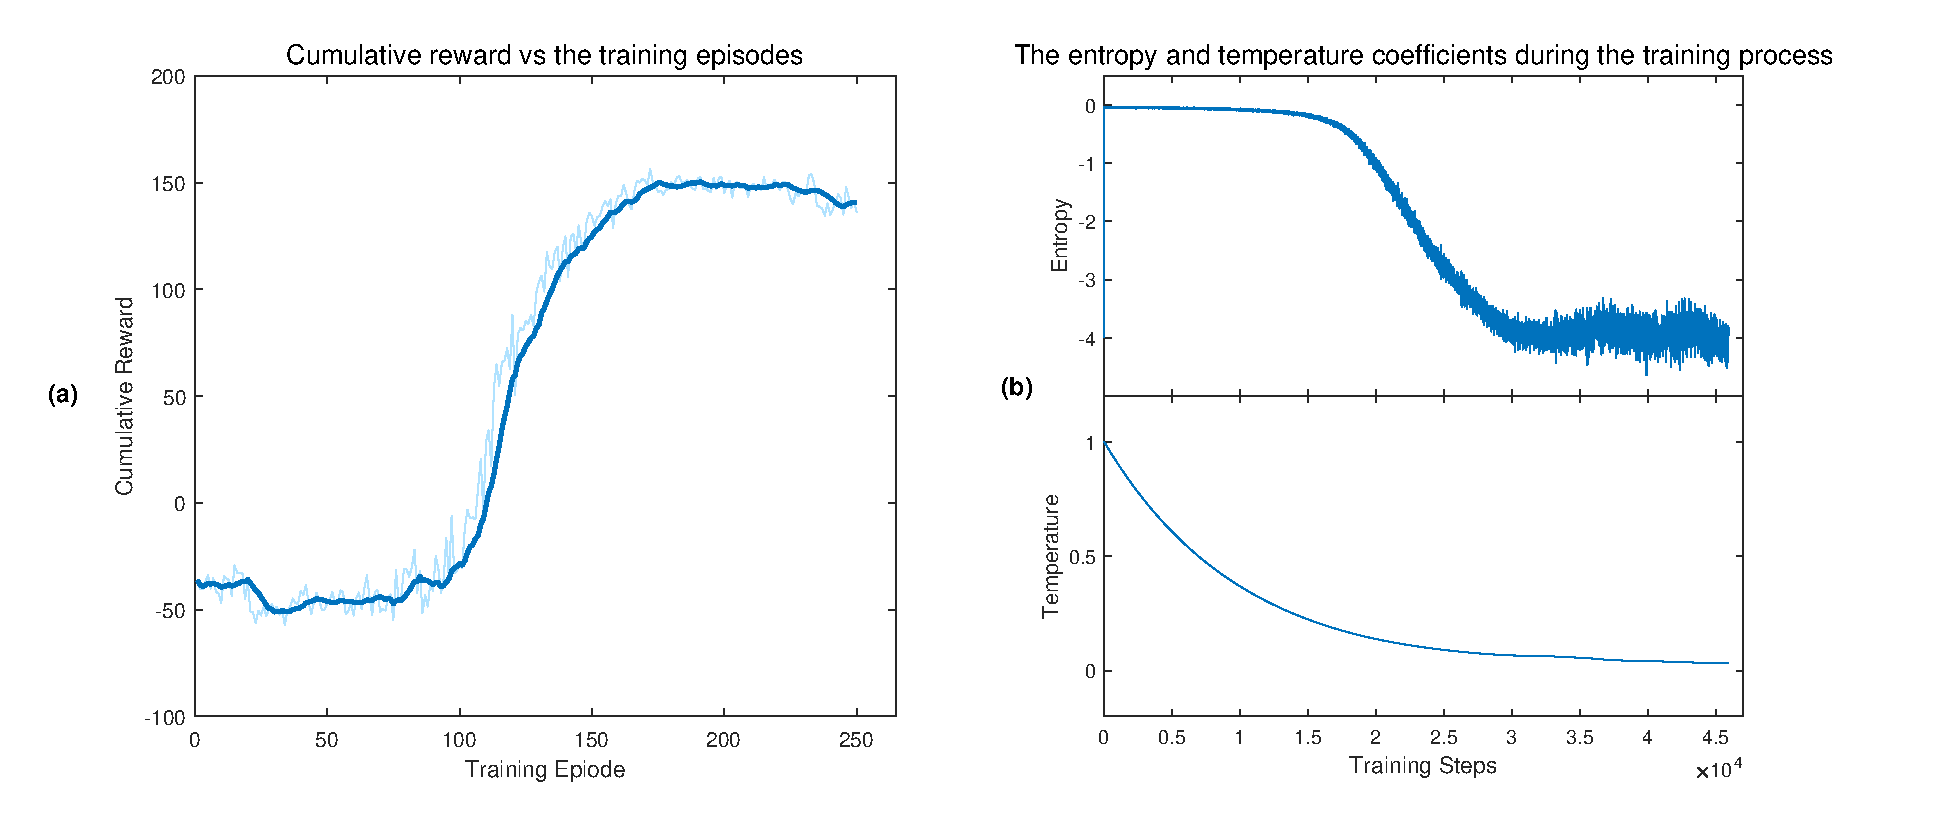
\includegraphics[width=\linewidth]{img/chap5/MBRL_tr.eps}
    \caption{The Training Results of MBRL. (a) Cumulative reward in MBRL vs the training episodes; (b) The variation of entropy and temperature parameters during the training process.}
    \label{fig:MBRL_tr}
\end{figure}

The training progress, along with the entropy and temperature parameters, is visually represented in Figure \ref{fig:MBRL_tr}. The plot illustrates the successful training of the agent using the SAC algorithm. The cumulative reward steadily increased from approximately -45 to 150, indicating the acquisition of the desired behavior by the agent. Additionally, the entropy decreased to around -4 (with the goal being the negative of the number of actions), and the temperature parameter also exhibited a decline from 1 to 0.05. These trends signify that the agent effectively learned the desired behavior during the training phase. Subsequent to the training process, the trained agent was implemented in simulation to evaluate its performance. The results of this implementation are elucidated in Figure \ref{fig:MBRL_val}, providing valuable insights into how well the trained MBRL model performs in executing optimal gaits for the SoftQ. 

Post-training validation in the simulation environment, conducted for a duration of 5 seconds, yielded noteworthy observations. As depicted in the figure, the robot exhibited some velocity along the x-axis. However, it remained virtually stationary at its initial position, effectively patrolling within a confined area. Despite generating speed, the robot failed to manifest any significant forward displacement. This phenomenon is notably characterized by a marked increase in the \ac{COT} during the initial phases of robot motion. This surge in \ac{COT} can be attributed to the imperative need for the robot to surmount inertia and initiate acceleration as it commences motion. Consequently, a substantial input of energy is necessitated. Additionally, heightened frictional forces encountered by mechanical components, such as wheels and joints, during the initial moments of motion contribute to this increased energy expenditure. In addition, the COT is defined as $$COT = \frac{E}{md}$$ where $E$ is the energy consumed to walk, $m$ is the mass of the robot and $d$ represents the distance travelled by the robot.

\begin{figure}[htb]
    \centering
    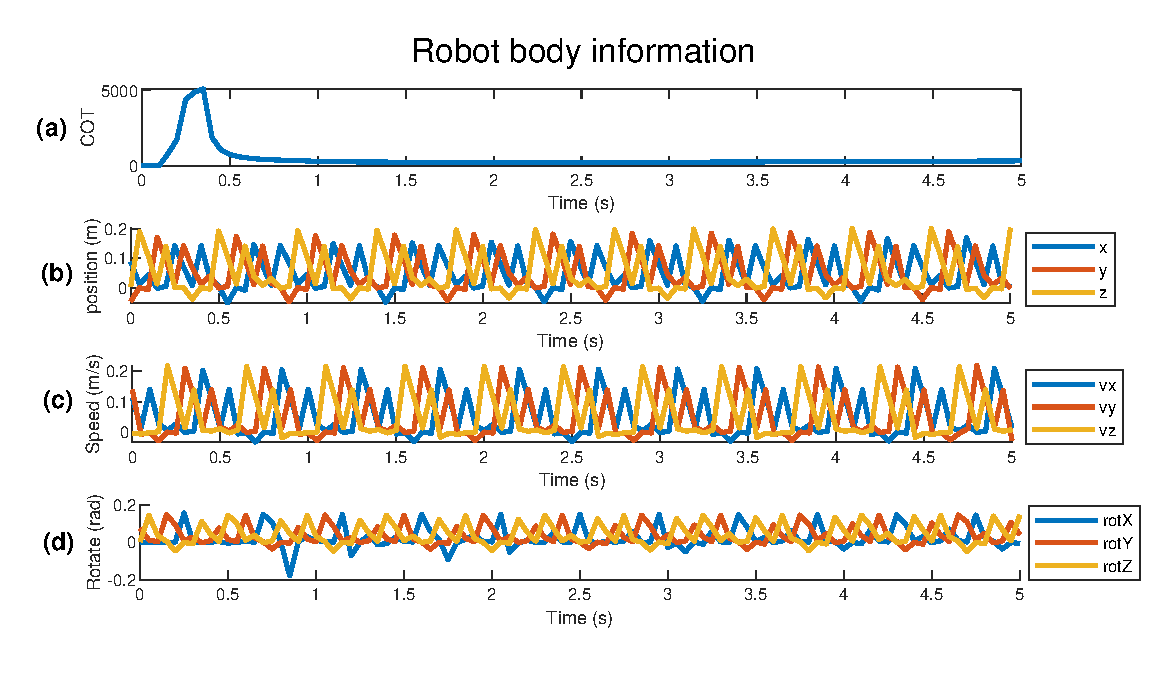
\includegraphics[width=\linewidth]{img/chap5/MBRL_val.eps}
    \caption{The Validation Results of MBRL. (a) COT of the robot while walking; (b) Distance traveled along the $x$, $y$, and $z$ axis; (c) Speed of the robot along the $x$, $y$, and $z$ axis; (d) Orientation of the robot along the $x$, $y$, and $z$ axis.}
    \label{fig:MBRL_val}
\end{figure}

To assess the operational capacity and explore the gait patterns of the soft robot, the same RL configurations were applied to learn optimal gaits under different reference speeds denoted as $v_{ref}$. Throughout the training experiments, an interesting observation emerged: the training performance of the simulated robot was notably influenced by the reference speed $v_{ref}$. When the target velocity was set higher, the learning agent was able to achieve forward motion in fewer training episodes, ultimately converging to an effective policy. Conversely, when $v_{ref}$ was set to a lower value, the agent exhibited a tendency to pitch forward, resulting in episode termination. The training process was initiated with various random seeds, and it was observed that training had a higher failure rate when the agent became trapped in local minima. Consequently, it can be intuitively inferred that mastering the policy for low-speed locomotion posed a more challenging task for the agent.

Given the limitations observed in the direct application of the agent trained through MBRL, a decision was made to further train this agent in a model-free environment to bridge the reality gap effectively. It is noteworthy that adjustments were made to the reward structure, particularly in penalizing instances where all four legs bent in the same direction with a significant angle. The coefficient $\epsilon_4$ governing this penalty was increased from 10 to 100. This modification was introduced due to the possibility that the model-based training might generate actions that are fatal in simulation but less perilous in the real-world scenario.

\subsection{Continue Learning}
To accelerate the training process, a predefined expert behavior, denoted as $A^e = [\textbf{a}_{T_0}^e, ..., \textbf{a}_T^e]$, is established\cite{jiSynthesizingOptimalGait2022}. This predefined behavior offers the robot an initial stable gait. Specifically, during the initial second of each training episode, the RL agent emulates human knowledge by executing the predefined behavior $A^e$. By this means, we resort to the framework of \textit{imitate learning}\cite{koberImitationReinforcementLearning2010}. Data generated from this process is collected and stored in a replay buffer for subsequent learning phases. This approach aligns with the principles of imitation learning, where the RL agent imitates pre-established behaviors as a form of guidance. While it's important to note that this predefined state-action trajectory doesn't guarantee optimality, it serves as a valuable reference for the agent. Emulating these guided elementary movements enables the agent to swiftly implement and adapt its behavior in real-time scenarios, contributing to efficient online implementation. 

To continue training the agent from MBRL, the same RL configurations were applied, with the exception of the penalty adjustment for the four legs bending. The goal for the robot was to learn an optimal gait for higher speed, with $v_{ref}$ set at 0.3 m/s. The reward functions remained the same as defined in Equation \ref{eq:reward}, but the coefficients were adjusted to $[\epsilon_1, \epsilon_2, \epsilon_3, \epsilon_4, \epsilon_5] = [5, −1/v_{ref}, 0.25, 100, 3]$. 

The results of continue training are visualized in Figure \ref{fig:MFRLvsCT} for comparison with Model-Free Reinforcement Learning (MFRL). Notably, it is observed that the continue training policy exhibited rapid improvement, reaching convergence at around 200 episodes. However, it's important to note that this policy incurs higher penalties, aligning with the assumption that the MBRL policy may generate riskier actions. Additionally, the MFRL policy converges at approximately 120 episodes, which is slower than the continue training agent. However, the reward at the beginning of training is higher for MFRL, indicating that the agent in early training may not actively promote forward motion but is associated with fewer high-risk actions. Furthermore, the MFRL approach failed to converge to a walking gait even after 400 episodes, and the MFRL agent did not learn to travel a significant distance. Notably, the MFRL method required about 24 hours of training, while MBRL and continue training together took approximately 10.5 hours. This substantial reduction in training time, coupled with the ability to achieve effective learning and improved gait control, underscores the efficiency and effectiveness of the continue training approach compared to the benchmark MFRL method.
\begin{figure}[htb]
    \centering
    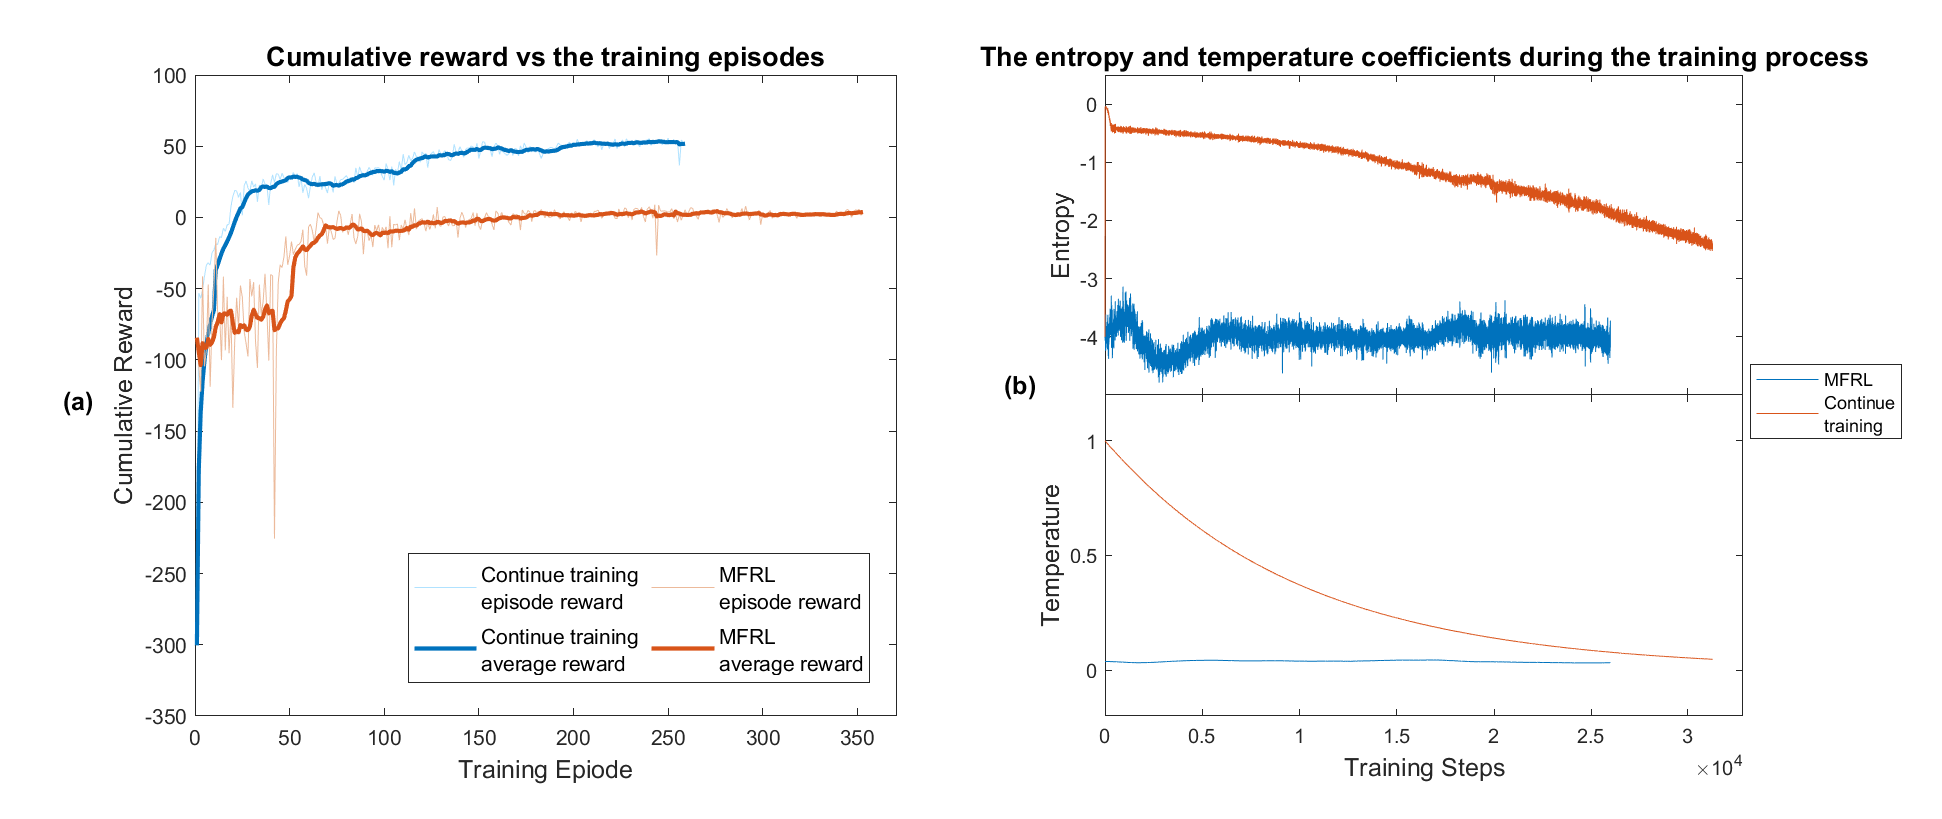
\includegraphics[width=\linewidth]{img/chap5/MFRLvsCT.eps}
    \caption{The Training Results of Continue Training Compared to MFRL. (a) Cumulative reward in MFRL and continue training vs the training episodes; (b) The variation of entropy and temperature coefficients during the training process of both MFRL and continue training.}
    \label{fig:MFRLvsCT}
\end{figure}

The outcomes of validations for continue training are graphically presented in Figure \ref{fig:CT}, which serves as a overview of continue training performance. The COT achieved a remarkable low value of approximately 73 J/kg/m, signifying the robot's ability to traverse a certain distance with efficient energy consumption. Over a 5-second validation period, the robot covered a distance of 1.8 meters, achieving an average speed of 0.36 m/s, surpassing the reference speed of 0.3 m/s. These findings highlight the agent's capability to attain and sustain a speed higher than the predefined benchmark. Moreover, the robot demonstrated stability during locomotion, as indicated by the minor fluctuations in velocity along the $x$-axis and minimal deviations in the $y$ and $z$ axes. The orientation plots revealed controlled movement, with the largest rotation measuring approximately 0.055 radians in the initial stages, confirming a stable and well-maintained gait. Collectively, these validation results underscore the practical viability of the continue training technique in enhancing the robot's performance in real-world scenarios.

\begin{figure}[htb]
    \centering
    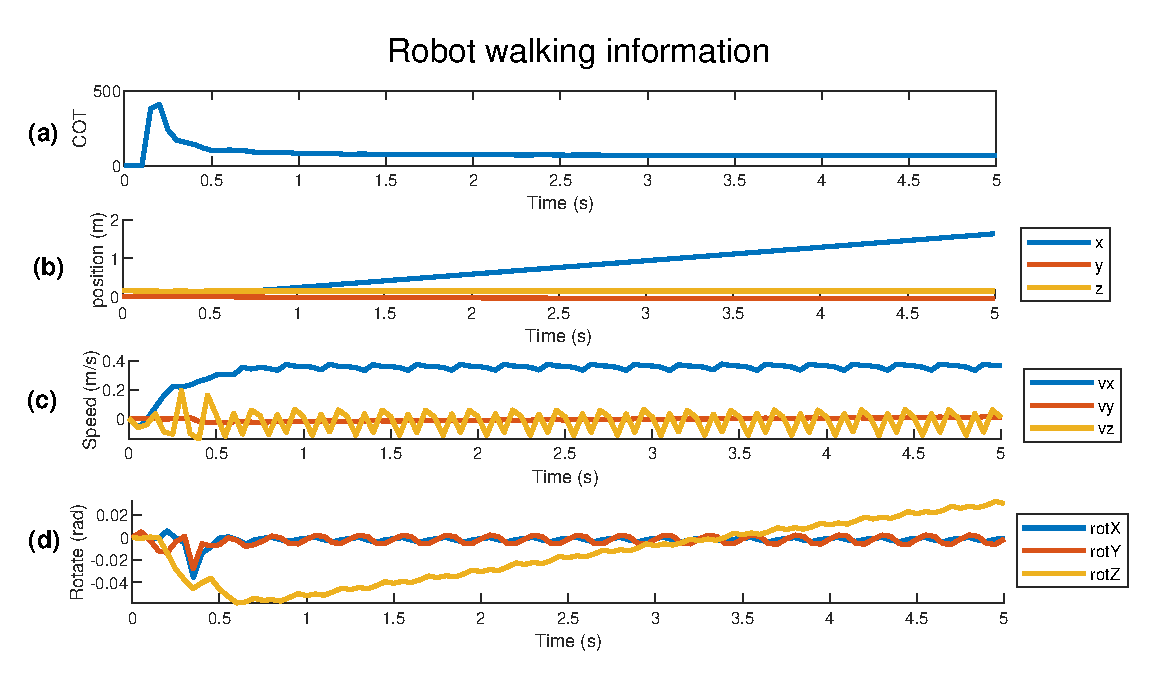
\includegraphics[width=0.9\linewidth]{img/chap5/best_CL.eps}
    \caption{The Validation Results of Continue Training. (a) COT of the robot while walking; (b) Distance traveled along the $x$, $y$, and $z$ axis; (c) Speed of the robot along the $x$, $y$, and $z$ axis; (d) Orientation of the robot along the $x$, $y$, and $z$ axis.}
    \label{fig:CT}
\end{figure}

Figure \ref{fig:CT_gait} (a) shows the examples of the four foot trajectories, and Figure \ref{fig:CT_gait} (b) with colored areas representing the contact regions demonstrates a typical gait patterns captured from the validation simulation. Synchronized motions were observed between the FR and RL legs, as well as the FL with RR legs, as they are linked as pairs. Notably, the FL and RR leg pairs exhibit a smaller swing area compared to the FR and RL pairs. This difference in swing area may be attributed to corrective actions addressing yaw rotation errors. These yaw rotation errors could potentially be caused by slight uneven mass distribution on the robot, favoring the right side, as indicated by the orientation in the $z$ axis shown in Figure \ref{fig:CT} (d). Additionally, a delay of approximately 0.1 seconds is observed between each diagonal leg pair. The contact time for each leg is around 0.15 seconds, resulting in the formation of a periodic gait pattern. This pattern indicates that the robot successfully learned to coordinate its movements in a rhythmic manner, which is essential for stable and sustained locomotion.

\begin{figure}[htb]
    \centering
    \begin{subfigure}[b]{0.45\textwidth}
    \centering
    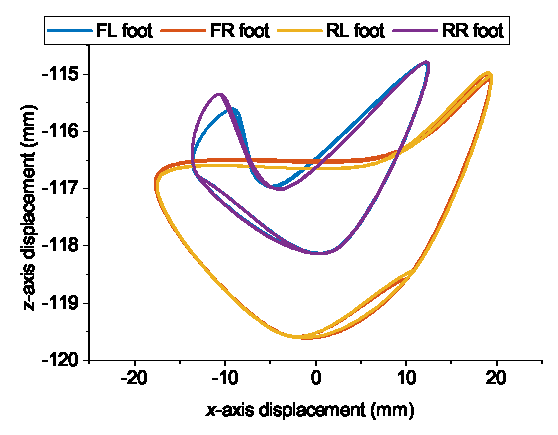
\includegraphics[width=\linewidth]{img/chap5/foot_trace.eps}
    \caption{}
    \end{subfigure}
    \begin{subfigure}[b]{0.45\textwidth}
    \centering
    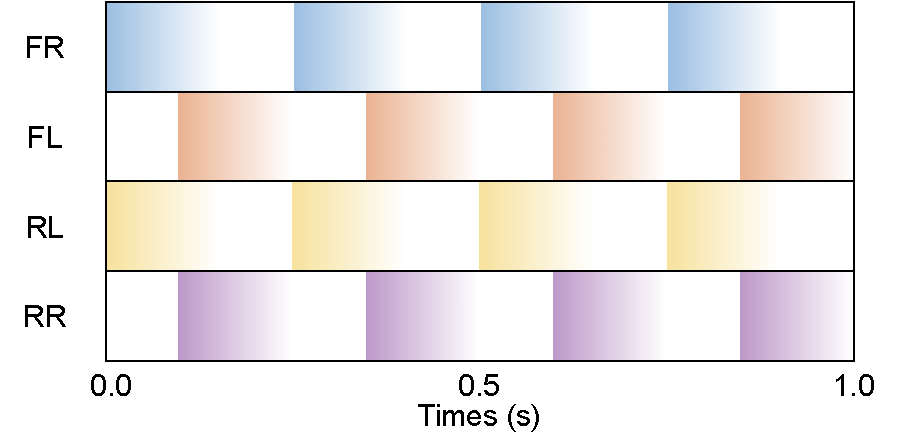
\includegraphics[width=\linewidth]{img/chap5/pattern.pdf}
    \caption{}
    \end{subfigure}
    \caption{The Learned gait patterns. (a) Four foot moving trajectories. (b) Footfall patterns}
    \label{fig:CT_gait}
\end{figure}

Moreover, it's essential to highlight that the observed results go beyond demonstrating successful gait patterns and stability. They also reveal the practical significance of this achievement in terms of direction control within velocity control. As shown in Figure \ref{fig:CT} (d), in the beginning of walking, the robot initially turns to the right but subsequently corrects itself, adjusting its orientation slightly to the left by the end of the gait cycle. This phenomenon was also observed in field tests, as presented in Section \ref{video}. This capability for self-correction and precise direction control enhances the robot's suitability for applications that require controlled and accurate movement, further expanding its utility in real-world scenarios. 

\section{Model-based RL Comparison}
\label{Sec:MBRL}

In order to examine the operational capacity and investigate the gait patterns of the soft robot, we applied the above RL setups to learn the walking motions with different speed references $v_{ref}$, where the training settings are identical in each experiment. During the training experiments, we observe that the training performance of the simulated robot is susceptible to the reference speed $v_{ref}$. With a higher target velocity, the agent is able to walk forward in fewer training episodes with a converged policy. On the other hand, with a smaller $v_{ref}$ as the target, the agent is prone to pitch forward and the episode is terminated. We start the training process with various random seeds, and the training has a higher failure rate with the agent stuck in the local minimal. Hence intuitively, we regard mastering the low-speed locomotion policy as a more difficult task for the agent.

\subsection{Performance Evaluation}
In the performance evaluation of the trained agent, it is important to consider several critical metrics. These metrics serve as crucial indicators of proficiency of the agent, referred to as the controller. Here, these metrics are expounded again avoiding excessive details:
\begin{itemize}
    \item Stability : This metric combines information about the time duration of the gait, rotational motion, and vertical displacement to assess the stability of the gait. It provides valuable insights into the agent's ability to maintain stability during operation. 
    \item Resultant walking speed (m/s): This metric involves assessing the agent's walking speed, particularly by calculating the average speed achieved during validation. It offers a straightforward measure of the agent's mobility and effectiveness in movement.
    \item Cost-of-Transport (J/kg/m):  The COT metric evaluates the energy efficiency of the agent. It quantifies the amount of energy expended by the agent, normalized by its weight and the distance traveled. This metric is crucial for understanding the agent's energy consumption patterns.
    \item Learning efficiency:  Learning efficiency gauges how quickly the agent converges to an optimal or satisfactory performance level. It is quantified by measuring the training time required for the agent to reach convergence and the reward reach a significant level. This metric provides insights into the agent's adaptability and learning capabilities.
\end{itemize}

\subsection{Compare with MFRL}
This section will delve into the performance comparison between the MBRL with continue training and MFRL based metrics outlined earlier. To ensure a robust evaluation, three identical training sessions were conducted for each reference velocity $v_{ref}$, which took values of 0.2 m/s, 0.3 m/s, and 0.5 m/s. Training was stopped upon the convergence of each policy to a significant reward level. Following the training phase, each trained agent was implemented and evaluated through simulation of 5s. The results of these evaluations are visually represented in Figure \ref{fig:box}. It is evident from the figure that MBRL with continuous training consistently outperforms MFRL. This conclusion is drawn based on the observation that the mean values of key performance metrics, including stability, resultant walking speed, COT, and training time, are consistently higher for MBRL with continuous training compared to MFRL.

\begin{figure}[htb]
    \centering
    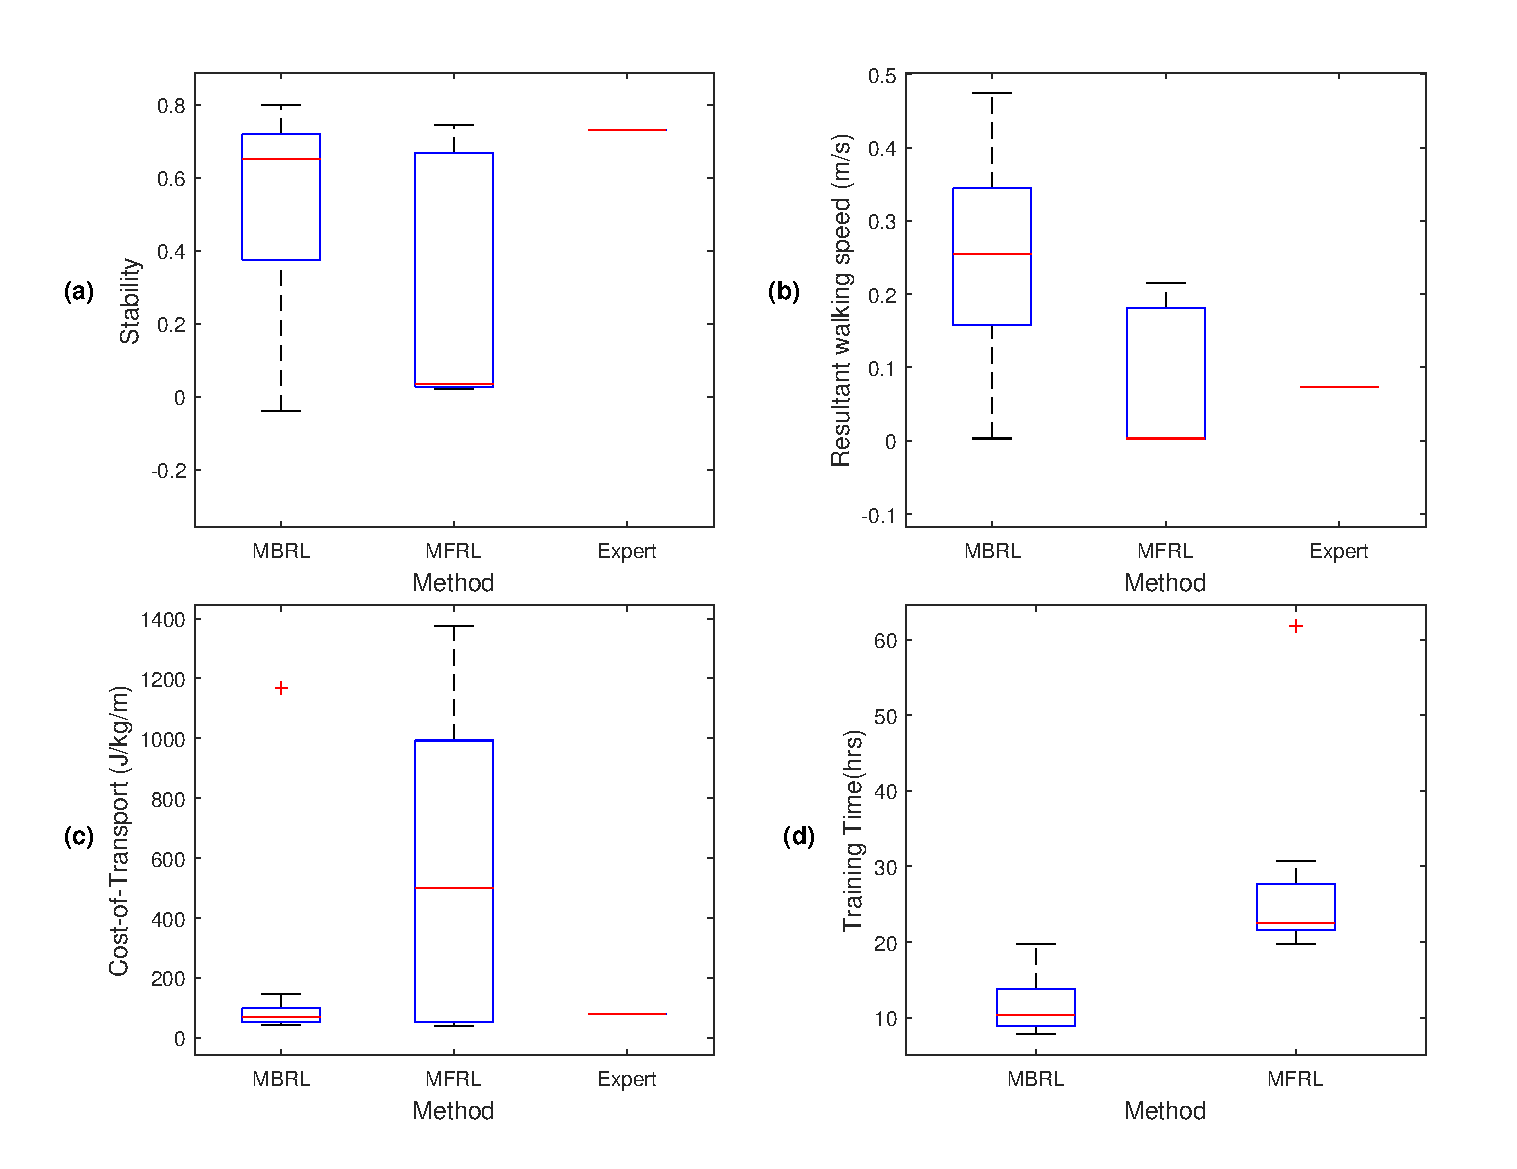
\includegraphics[width=\linewidth]{img/chap5/box_results.eps}
    \caption{The Box Plot of MBRL with Continue Training compared to MFRL. (a) Box plot of stability by method; (b) Box plot of resultant walking speed by method ; (c) Box plot of COT by method; (d) Box plot of simulation time by method.}
    \label{fig:box}
\end{figure}

However, it is essential to acknowledge that reference walking speed ($v_{ref}$) represents a covariate in this comparative analysis. To ensure a rigorous assessment that accounts for the potential influence of this covariate, an \ac{ANCOVA} was conducted to compare MBRL with continue learning and MFRL. This statistical analysis enabled us to compare these two RL approaches while effectively controlling for the covariate $v_{ref}$. This analysis primarily focused on the following dependent variables, as previously defined in Section \ref{Sec:test_def}: stability, resultant walking speed, COT and learning efficiency. This ANCOVA analysis provides a robust framework for evaluating the relative performance of the two RL approaches, while considering the potential impact of reference walking speed ($v_{ref}$). The results of this analysis offer deeper insights into the effectiveness of each method in achieving stable and efficient gait control for our soft robot. The details of ANCOVA is discussed in \ref{Sec:ANCOVA}.

The hypothesis holds that MBRL with continue training is significantly more effective and efficient in achieving stable and efficient gait control for our soft robot SoftQ compared to MFRL, across various reference velocities ($v_{ref}$).

\subsubsection*{Stability}
The ANCOVA analysis revealed both the method of RL (MBRL or MFRL) and the covariate $v_{ref}$ have a statistically significant effect on walking stability. The F-value of 5.9902 and the p-value of 0.0307 in the effect of method indicate that the method of RL significantly influences walking stability. Given that the p-value is less than 0.05, this effect is statistically significant, suggesting that one of these methods is likely better than the other in terms of enhancing walking stability. $v_{ref}$ serves as a covariate in this study, and it too shows a statistically significant F-value of 4.3583 and a p-value of 0.0378. This implies that $v_{ref}$ independently impacts walking stability, and its effect is statistically significant. The interaction between the method and $v_{ref}$ is also significant, with an F-value of 5.4802 and a p-value of 0.0204. This suggests that the effect of the learning method on walking stability is not consistent across all levels of $v_{ref}$. In other words, the optimal choice between MBRL and MFRL may depend on the specific value of $v_{ref}$. This suggests that the  RL approaches has a significant positive impact on the stability of walking.

\begin{table}[H]
    \centering
    \begin{tabular}{c|ccccc} 
         Source&  DoF&  Sum Sq&  Mean Sq&  F& Prob>F\\ \hline
         $v_{ref}$&  2&  0.4734&  0.2367&  4.3583& 0.0378\\ 
         Method&  1&  0.3254&  0.3254&  5.9902& 0.0307\\ 
         $v_{ref}\cdot$Method&  2&  0.5953&  0.2977&  5.4802& 0.0204\\ 
         Error&  12&  0.6518&  0.0543&  & \\ 
    \end{tabular}
    \caption{ANCOVA test of stability metrics.}
    \label{tab:ANCOVA_sta}
\end{table}

\subsubsection*{Resultant walking speed}
The ANCOVA analysis concluded that the method of RL significantly impacts resultant walking speed, while $v_{ref}$ does not. The DoF for $v_{ref}$ is 2, and it has a Sum of Squares (Sum Sq) of 0.0056, yielding a Mean Square (Mean Sq) of 0.0028. The F-value is a low 0.2133, and the p-value is notably high at 0.8109. These metrics strongly suggest that $v_{ref}$ does not have a statistically significant impact on the resultant walking speed in this case. The Method has a DoF of 1 with a Sum Sq of 0.1390, resulting in a Mean Sq of 0.1390. The F-value is considerably high at 10.6660, and the p-value is 0.0068, well below the 0.05 threshold. These values point to a statistically significant influence of the RL method on resultant walking speed. This implies that either MBRL or MFRL has a substantial impact on walking speed, warranting further investigation to determine the most effective approach. The interaction term shows a DoF of 2, a Sum Sq of 0.0991, and a Mean Sq of approximately 0.0496. With an F-value of 3.8011 and a p-value of 0.0526, the interaction term is borderline significant. This indicates that the effect of the RL method on resultant walking speed may vary depending on $v_{ref}$, although the evidence is not strong enough to make this conclusion definitively.
\begin{table}[H]
    \centering
    \begin{tabular}{c|ccccc} 
         Source&  DoF&  Sum Sq&  Mean Sq&  F& Prob>F\\ \hline
         $v_{ref}$&  2&  0.0056&  0.0028&  0.2133& 0.8109\\ 
         Method&  1&  0.1390&  0.1390&  10.6660& 0.0068\\ 
         $v_{ref}\cdot$Method&  2&  0.0991&  0.0496&  3.8011& 0.0526\\ 
         Error&  12&  0.1564&  0.0130&  & \\ 
    \end{tabular}
    \caption{ANCOVA test of resultant walking speed.}
    \label{tab:ANCOVA_v}
\end{table}

\subsubsection{Cost-of-Transport}
The data indicates that the choice of RL method (MBRL or MFRL) has a statistically significant impact on COT. On the other hand, the influence of $v_{ref}$ is borderline significant, and the interaction term between $v_{ref}$ and method of RL is not statistically significant. In effect of $v_{ref}$, the F-value stands at 3.7479 with a p-value of 0.0544. While the F-value suggests a reasonable effect, the p-value marginally exceeds the typical 0.05 significance threshold, making the influence of $v_{ref}$ on COT statistically borderline. In effect of RL method, the F-value is 5.5947 with a p-value of 0.0357. Given the p-value is less than 0.05, the influence of the chosen RL method on COT is statistically significant. In the effect of interaction term ($v_{ref}\cdot$Method), the F-value is 2.9587, and the p-value is 0.0902. Although the F-value suggests some degree of effect, the p-value is greater than 0.05, suggesting that the interaction effect is not statistically significant. Therefore, while the RL method appears to be a crucial factor affecting COT, the role of $v_{ref}$ and its interaction with the method may require additional research to be conclusively understood.
\begin{table}[H]
    \centering
    \begin{tabular}{c|ccccc} 
         Source&  DoF&  Sum Sq&  Mean Sq&  F& Prob>F\\ \hline
         $v_{ref}$&  2&  \num{9.5553e5}&  \num{4.7776e5}&  3.7479& 0.0544\\ 
         Method&  1&  \num{7.1318e5}&  \num{7.1318e5}&  5.5947& 0.0357\\ 
         $v_{ref}\cdot$Method&  2&  \num{7.5432e5}&  \num{3.7716e5}&  2.9587& 0.0902\\ 
         Error&  12&  \num{1.5297e6}&  \num{1.747e5}&  & \\ 
    \end{tabular}
    \caption{ANCOVA test of COT.}
    \label{tab:ANCOVA_COT}
\end{table}

\subsubsection{Learning efficiency}
The ANCOVA analysis underscores the statistical significance of the RL method in influencing learning efficiency. The $v_{ref}$ term as a covariate,  is characterized by a Degrees of Freedom (DoF) of 2, Sum of Squares (Sum Sq) of 208.0905, and Mean Square (Mean Sq) of 104.0452. The F-value is 1.2107 and the p-value is 0.3319. Given the p-value is well above the common 0.05 significance threshold, $v_{ref}$ does not appear to have a statistically significant impact on learning efficiency. The Method term has a DoF of 1, a Sum Sq of \num{1.1997e3}, and a Mean Sq of \num{1.1997e3}. The F-value is remarkably high at 13.9597, and the p-value is notably low at 0.0028. These values confirm that the Method is statistically significant in affecting learning efficiency, suggesting a noteworthy influence of the chosen RL approach. The interaction term has a DoF of 2, a Sum Sq of 265.9588, and a Mean Sq of 132.9794. The F-value is 1.5473, and the p-value is 0.2524. These numbers indicate that the interaction term does not meet the threshold for statistical significance, which implies that the effect of the RL method on learning efficiency is generally consistent across different $v_{ref}$ levels. 
 
\begin{table}[H]
    \centering
    \begin{tabular}{c|ccccc} 
         Source&  DoF&  Sum Sq&  Mean Sq&  F& Prob>F\\ \hline
         $v_{ref}$&  2&  208.0905&  104.0452&  1.2107& 0.3319\\ 
         Method&  1&  \num{1.1997e3}&  \num{1.1997e3}&  13.9597& 0.0028\\ 
         $v_{ref}\cdot$Method&  2&  265.9588&  132.9794&  1.5473& 0.2524\\ 
         Error&  12&  \num{1.0313e3}&  85.9405&  & \\ 
    \end{tabular}
    \caption{ANCOVA test of learning efficiency.}
    \label{tab:ANCOVA_time}
\end{table}

\section{Field Test}
The culmination of the MBRL and continue training efforts is the deployment of the trained controller onto the physical SoftQ robot. This section presents the results of the field tests, providing insights into the controller's transferability, generalization capabilities, and its performance in real-world scenarios.

The primary objective of the field tests is to assess the extent to which the controller's learned motor skills can be transferred from the simulated environment to the physical robot. The results demonstrate the remarkable transferability and generalization capabilities of the trained controller. Despite the disparities between the simulation and the real world, the controller seamlessly applies the acquired behaviors in tangible, real-world settings.

\begin{figure}[htb]
    \centering
    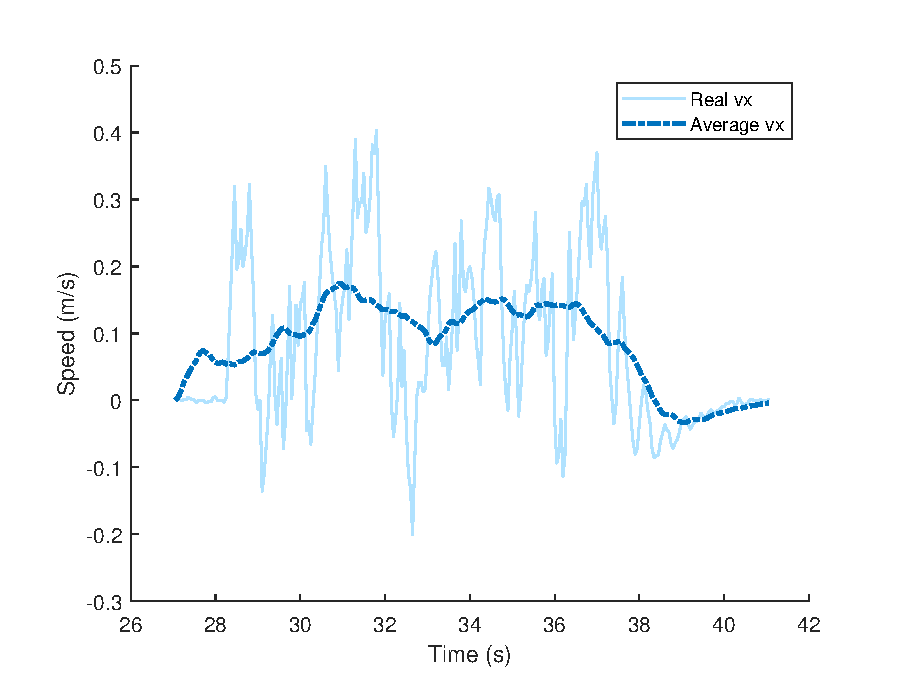
\includegraphics[width=0.9\linewidth]{img/chap5/real_vx.eps}
    \caption{The Field Test Results of Measurement of Velocity at $x$ axis.}
    \label{fig:real_vx}
\end{figure}

One of the key performance metrics evaluated during the field tests is the robot's locomotion. The trained controller showcases impressive locomotion performance across a range of terrains and conditions. It effectively adapts its gait and motor control to navigate flat surfaces, uneven terrain, slopes, and surfaces with varying friction properties. The controller's ability to maintain stability and achieve locomotion is a testament to its adaptability and robustness.

The outstanding performance observed in the field tests holds significant implications for the power of this methodology enhanced by MBRL. The robot prototype successfully completes the preliminary walking test under real-time execution by utilizing the SAC trained agents.
\chapter{Conclusions}
\label{chap6}
\textit{Describe the conclusions (reflect on the whole introduction given in Chapter 1). Discuss the positive effects and the drawbacks. Describe the evaluation of the results of the degree project. Describe valid future work. The sections below are optional but could be added here.}

\section{Discussion}
In conclusion, this research endeavor has sought to unravel the complexities surrounding gait control in soft quadruped robots, aiming to enhance our understanding and pave the way for more effective control strategies. Through a systematic exploration of the research questions outlined in this study, we have unearthed valuable insights and findings that contribute to the field of robotics and autonomous locomotion.

Our investigation into methods for restricting the state space and designing surrogate models with high estimation accuracy has revealed innovative approaches such as pattern-defined reinforcement learning and parameterization. These methods provide a solid foundation for efficient and accurate simulations and training, ultimately leading to improved gait control strategies.

Furthermore, the comparative analysis between model-based and model-free reinforcement learning approaches has shed light on the potential of the former in generating superior control agents for soft quadruped robots. The enhancements in stability, walking speed, and cost-of-transport underscore the significance of model-based reinforcement learning as a benchmark in this project. The careful consideration of trade-offs among learning efficiency, simulation accuracy, and long-term planning accuracy has provided essential insights into the quest for optimal gait control policies.

\section{Future Work}

An intriguing fact of our approach resides in the capacity to tailor the controller's behavior to various task objectives through the manipulation of distinct reward functions within the RL framework. By delineating specific reward functions, the RL algorithm learns to optimize the controller for diverse tasks of interest. This adaptability renders the methodology versatile and applicable to a spectrum of scenarios, allowing the robotic system to be endowed with a repertoire of task-specific skills.

This thesis has ventured into the realm of gait control for soft quadruped robots, uncovering valuable insights and paving the way for further investigations. As with any scientific endeavor, there are promising avenues for future research that can expand upon the knowledge and limitations identified in this study. In this section, we outline potential directions for future research in the field of soft quadruped robot gait control.

1. Real-world Validation

While this research primarily focused on simulation-based gait control, an imperative direction for future research involves the validation of control strategies in real-world scenarios. Conducting experiments with physical soft quadruped robots can bridge the gap between simulated environments and practical applications, enabling a more comprehensive assessment of control strategies and their effectiveness in real-world conditions.

2. Hardware Advancements

The continuous evolution of soft robotic materials and actuators presents an opportunity for future research. Investigating the integration of cutting-edge soft robotics hardware, such as novel actuators and sensors, can enhance the physical capabilities and adaptability of quadruped robots, thereby advancing their locomotion control.

3. Hybrid Control Strategies

Future research can explore the development of hybrid control strategies that combine the strengths of model-based and model-free reinforcement learning techniques. Such an approach may leverage the accuracy of model-based methods while retaining the adaptability and robustness of model-free techniques, offering a more versatile and reliable solution for gait control.

4. Multi-Terrain Adaptation

Soft quadruped robots are designed to navigate diverse terrains. Future research should prioritize the development of control algorithms that enable seamless adaptation to various surfaces, including rough, uneven, and dynamically changing terrains. This will expand the practical utility of soft quadruped robots across a wide range of environments.

5. Online Learning and Adaptation

Implementing online learning and adaptation mechanisms is crucial for enhancing a robot's ability to respond to changing environmental conditions and unforeseen challenges. Future research can focus on developing algorithms that allow soft quadruped robots to continuously update their control policies in real-time, improving their adaptability and performance.

6. Human-Robot Interaction

As soft quadruped robots find applications in human-centric environments, investigating human-robot interaction aspects becomes essential. Future research can explore how these robots can effectively collaborate with humans in tasks such as search and rescue, healthcare, logistics, and more, ensuring safe and seamless integration.

7. Energy Efficiency

Optimizing the energy efficiency of gait control is paramount, particularly for applications with limited battery resources. Future work should concentrate on developing control strategies that minimize energy consumption while maintaining or even enhancing performance, addressing a critical aspect of practical robot deployment.

8. Robustness and Fault Tolerance

Future research should delve into robust control strategies capable of withstanding disturbances and uncertainties in real-world scenarios. Additionally, investigating fault-tolerant control mechanisms to handle hardware failures or damage will be essential for ensuring the reliability of soft quadruped robots.

9. Multi-Robot Coordination

In scenarios involving multiple soft quadruped robots, coordinating their actions effectively is a complex challenge. Future research can explore techniques for multi-robot coordination, facilitating collaborative tasks in domains such as surveillance, exploration, and disaster response.

10. Ethical Considerations

As soft quadruped robots become integrated into society, ethical considerations, including privacy, safety, and their impact on employment, require careful examination. Future research should delve into these ethical dimensions to ensure the responsible deployment of these robots.

\subsection{Final Words}
In these final words, it is crucial to acknowledge the collaborative efforts of researchers, engineers and innovators who continue to push the boundaries of robotics. The journey to master gait control in soft quadruped robots is ongoing, with numerous challenges and opportunities awaiting exploration.

In the grand scheme of scientific exploration, this research represents a small but significant stride toward unlocking the full potential of soft quadruped robots. It is our hope that the knowledge gained here will inspire further research and innovation, ultimately leading to the realization of highly capable and versatile soft quadruped robots that can navigate the complexities of our ever-changing world.

In closing, this thesis marks not an end, but rather a new beginning in the journey to harness the untapped potential of soft quadruped robots. May our collective efforts continue to drive progress, pushing the boundaries of what these remarkable machines can achieve.








% \include{content}
%TC:ignore
\newpage
% \addcontentsline{toc}{chapter}{References}
% \thispagestyle{plain}
% \setstretch{0.75}
% \fontsize{5}{0}
% \setlength\bibitemsep{0pt}
\printbibliography[heading=bibintoc]
% \setstretch{1.25}
\newpage
\appendix
\newpage

\captionsetup[figure]{font=small,skip=0pt}
\etocdepthtag.toc{mtappendix}
\etocsettagdepth{mtchapter}{none}
\etocsettagdepth{mtappendix}{subsection}
\etoctocstyle{1}{Appendix - Contents}
\tableofcontents
\pagestyle{plain}
\newpage
\pagenumbering{arabic}

\chapter{Detailed Explanations and Supplementary Results}
In this chapter, the detailed explanations of the concepts discussed in the main text and present supplementary results that contribute to a clearer overview of the key outcomes of this thesis. These additional findings provide valuable context and insights that complement the primary research findings.

\section{Quaternions to Euler Angles}
\label{sec:Q2E}
Even though Euler angles are used to represent rotations, the transmission of two poses are calculated by Quaternion, which is a mathematical construct that extends the notion of complex numbers to four dimensions. They comprise four components: a scalar part represented by $w$, and a vector component denoted as $\vec{v}=(x, y, z)$. Quaternions are expressed as:
$$q = w + xi + yj + zk$$
where $x$, $y$, $z$, and $w$ are real numbers, and $i$, $j$, and $k$ are three imaginary units that satisfy the following multiplication rules: $i^2 = j^2 = k^2 = ijk = -1$. This approach involves establishing the initial pose of the robot as a quaternion and subsequently updating the current pose through sensors like accelerometers and gyroscopes. By computing the difference between the initial and current poses, the rotational component of the transformation can be extracted. This rotational component is often represented as a 3x3 rotation matrix $R$, which can then be used to derive the Euler angles 'yaw', 'pitch', and 'roll', providing insights into the robot's orientation in three-dimensional space. 
$$ R = \begin{bmatrix}
1 - 2(y^2 + z^2) & 2(xy - wz) & 2(xz + wy) \\
2(xy + wz) & 1 - 2(x^2 + z^2) & 2(yz - wx) \\
2(xz - wy) & 2(yz + wx) & 1 - 2(x^2 + y^2)
\end{bmatrix}
$$
The conversion from the rotation matrix 'R' to Euler angles 'yaw', 'pitch', and 'roll' involves the following mathematical expressions:
\begin{align*}
\text{yaw (Y)} & = \text{atan2}(R_{21}, R_{11}) \\
\text{pitch (X)} & = -\text{asin}(R_{31}) \\
\text{roll (Z)} & = \text{atan2}(R_{32}, R_{33})
\end{align*}

\section{Kalman Filter Update}
\label{sec:kf}
The Kalman filter, a fundamental tool in state estimation for dynamic systems, continuously refines its state estimate in the presence of noisy measurements. This section provides an overview of the Kalman filter's update process, shedding light on its predictive and corrective steps.

\textbf{State Transition Model (Predictive Step):}
In the predictive step, the Kalman filter employs the system's dynamics to forecast the next state ($x_{k|k-1}$) based on the previous state estimate ($x_{k-1|k-1}$). This forecast hinges on a linear transformation captured by the state transition matrix ($A$):
\begin{equation*}
x_{k|k-1} = A \cdot x_{k-1|k-1}
\end{equation*}

The state covariance ($P_{k|k-1}$) is also updated to account for the inherent uncertainty in this prediction:
\begin{equation*}
P_{k|k-1} = A \cdot P_{k-1|k-1} \cdot A^T + Q
\end{equation*}
Here, $Q$ represents the process noise covariance matrix, characterizing the uncertainty introduced by the system dynamics.

\textbf{Measurement Update (Corrective Step):}
In the corrective step, measurements ($z_k$) are incorporated into the state estimate to enhance its accuracy. The Kalman gain ($K_k$) is computed to determine the weight assigned to the measurement versus the prediction:
\begin{equation*}
K_k = P_{k|k-1} \cdot H^T \cdot (H \cdot P_{k|k-1} \cdot H^T + R)^{-1}
\end{equation*}
In this equation, $H$ represents the measurement matrix, mapping the state to the measurement space. The measurement noise covariance matrix ($R$) captures the uncertainty associated with sensor measurements.

Leveraging the Kalman gain, the state estimate and its covariance are updated as follows:
\begin{align*}
x_{k|k} = x_{k|k-1} + K_k \cdot (z_k - H \cdot x_{k|k-1}) \
P_{k|k} = (I - K_k \cdot H) \cdot P_{k|k-1}
\end{align*}
In these equations, $I$ denotes the identity matrix. The Kalman filter's iterative process continually refines the state estimate and its associated uncertainty, making it a powerful tool for state estimation in the presence of noise and uncertainty..

\section{Single Step Prediction of two NNs}
\begin{figure}[htb]
    \centering
    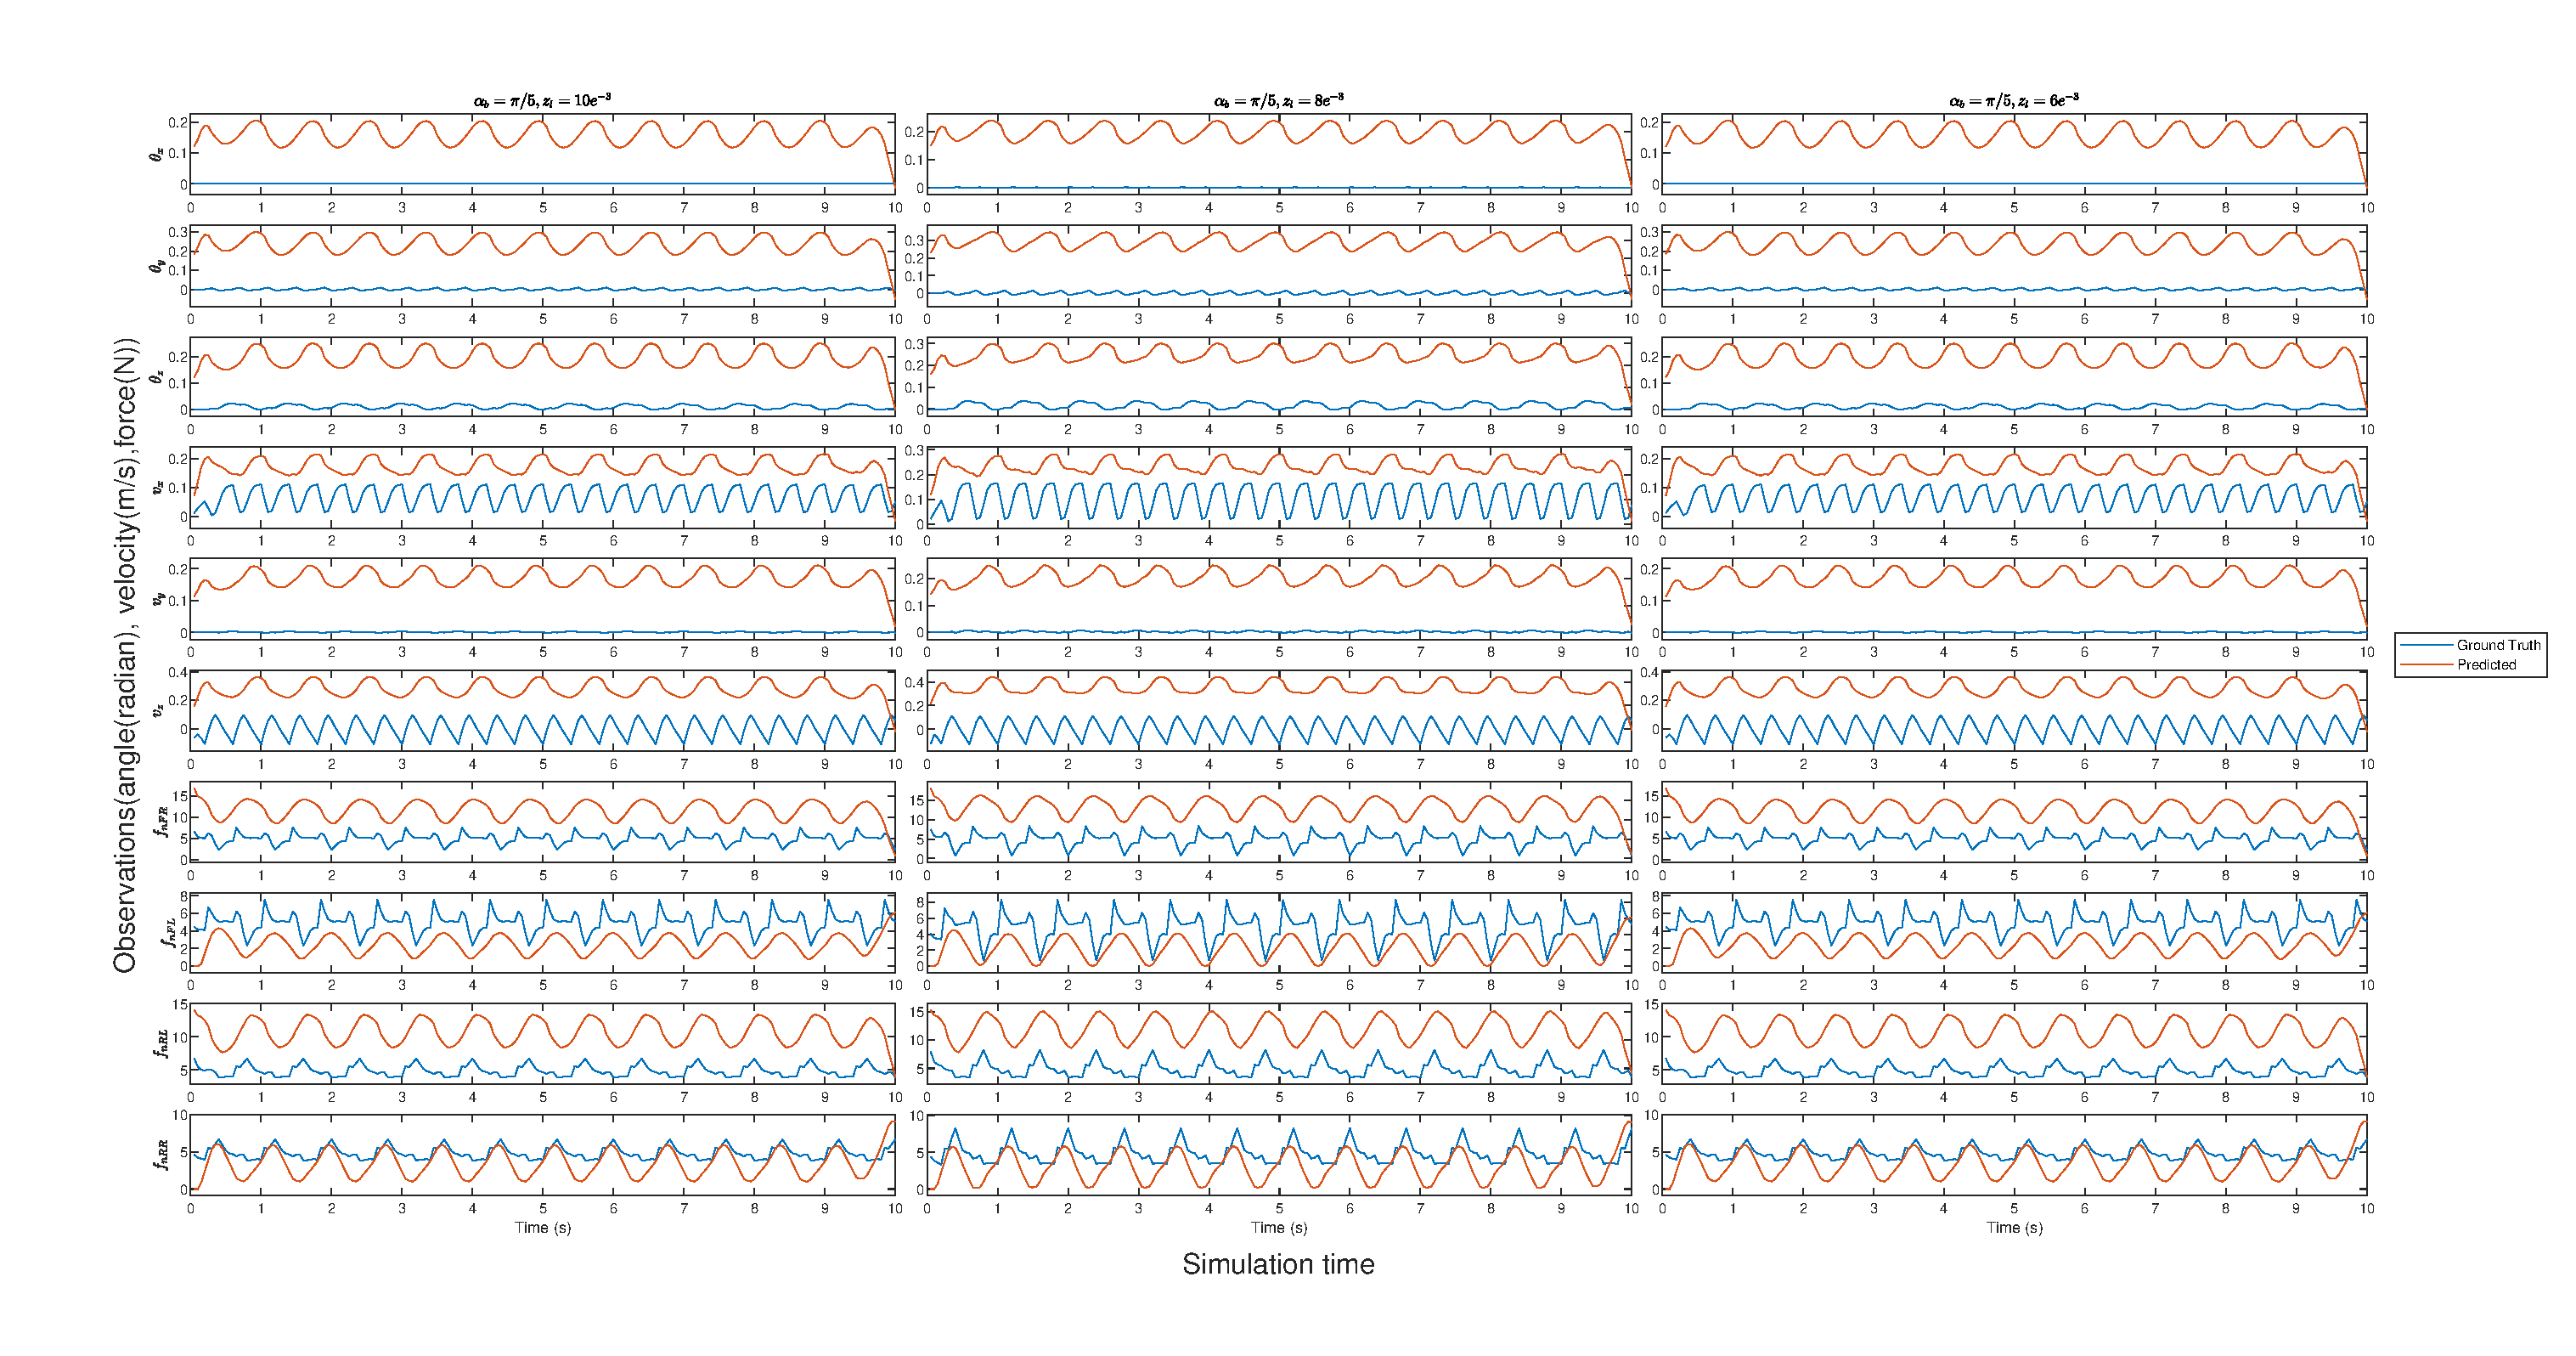
\includegraphics[width=\linewidth]{img/AppA/lstm_pred.eps}
    \caption{Single step prediction test of LSTM network}
    \label{fig:lstm_test}
\end{figure}

\begin{figure}[htb]
    \centering
    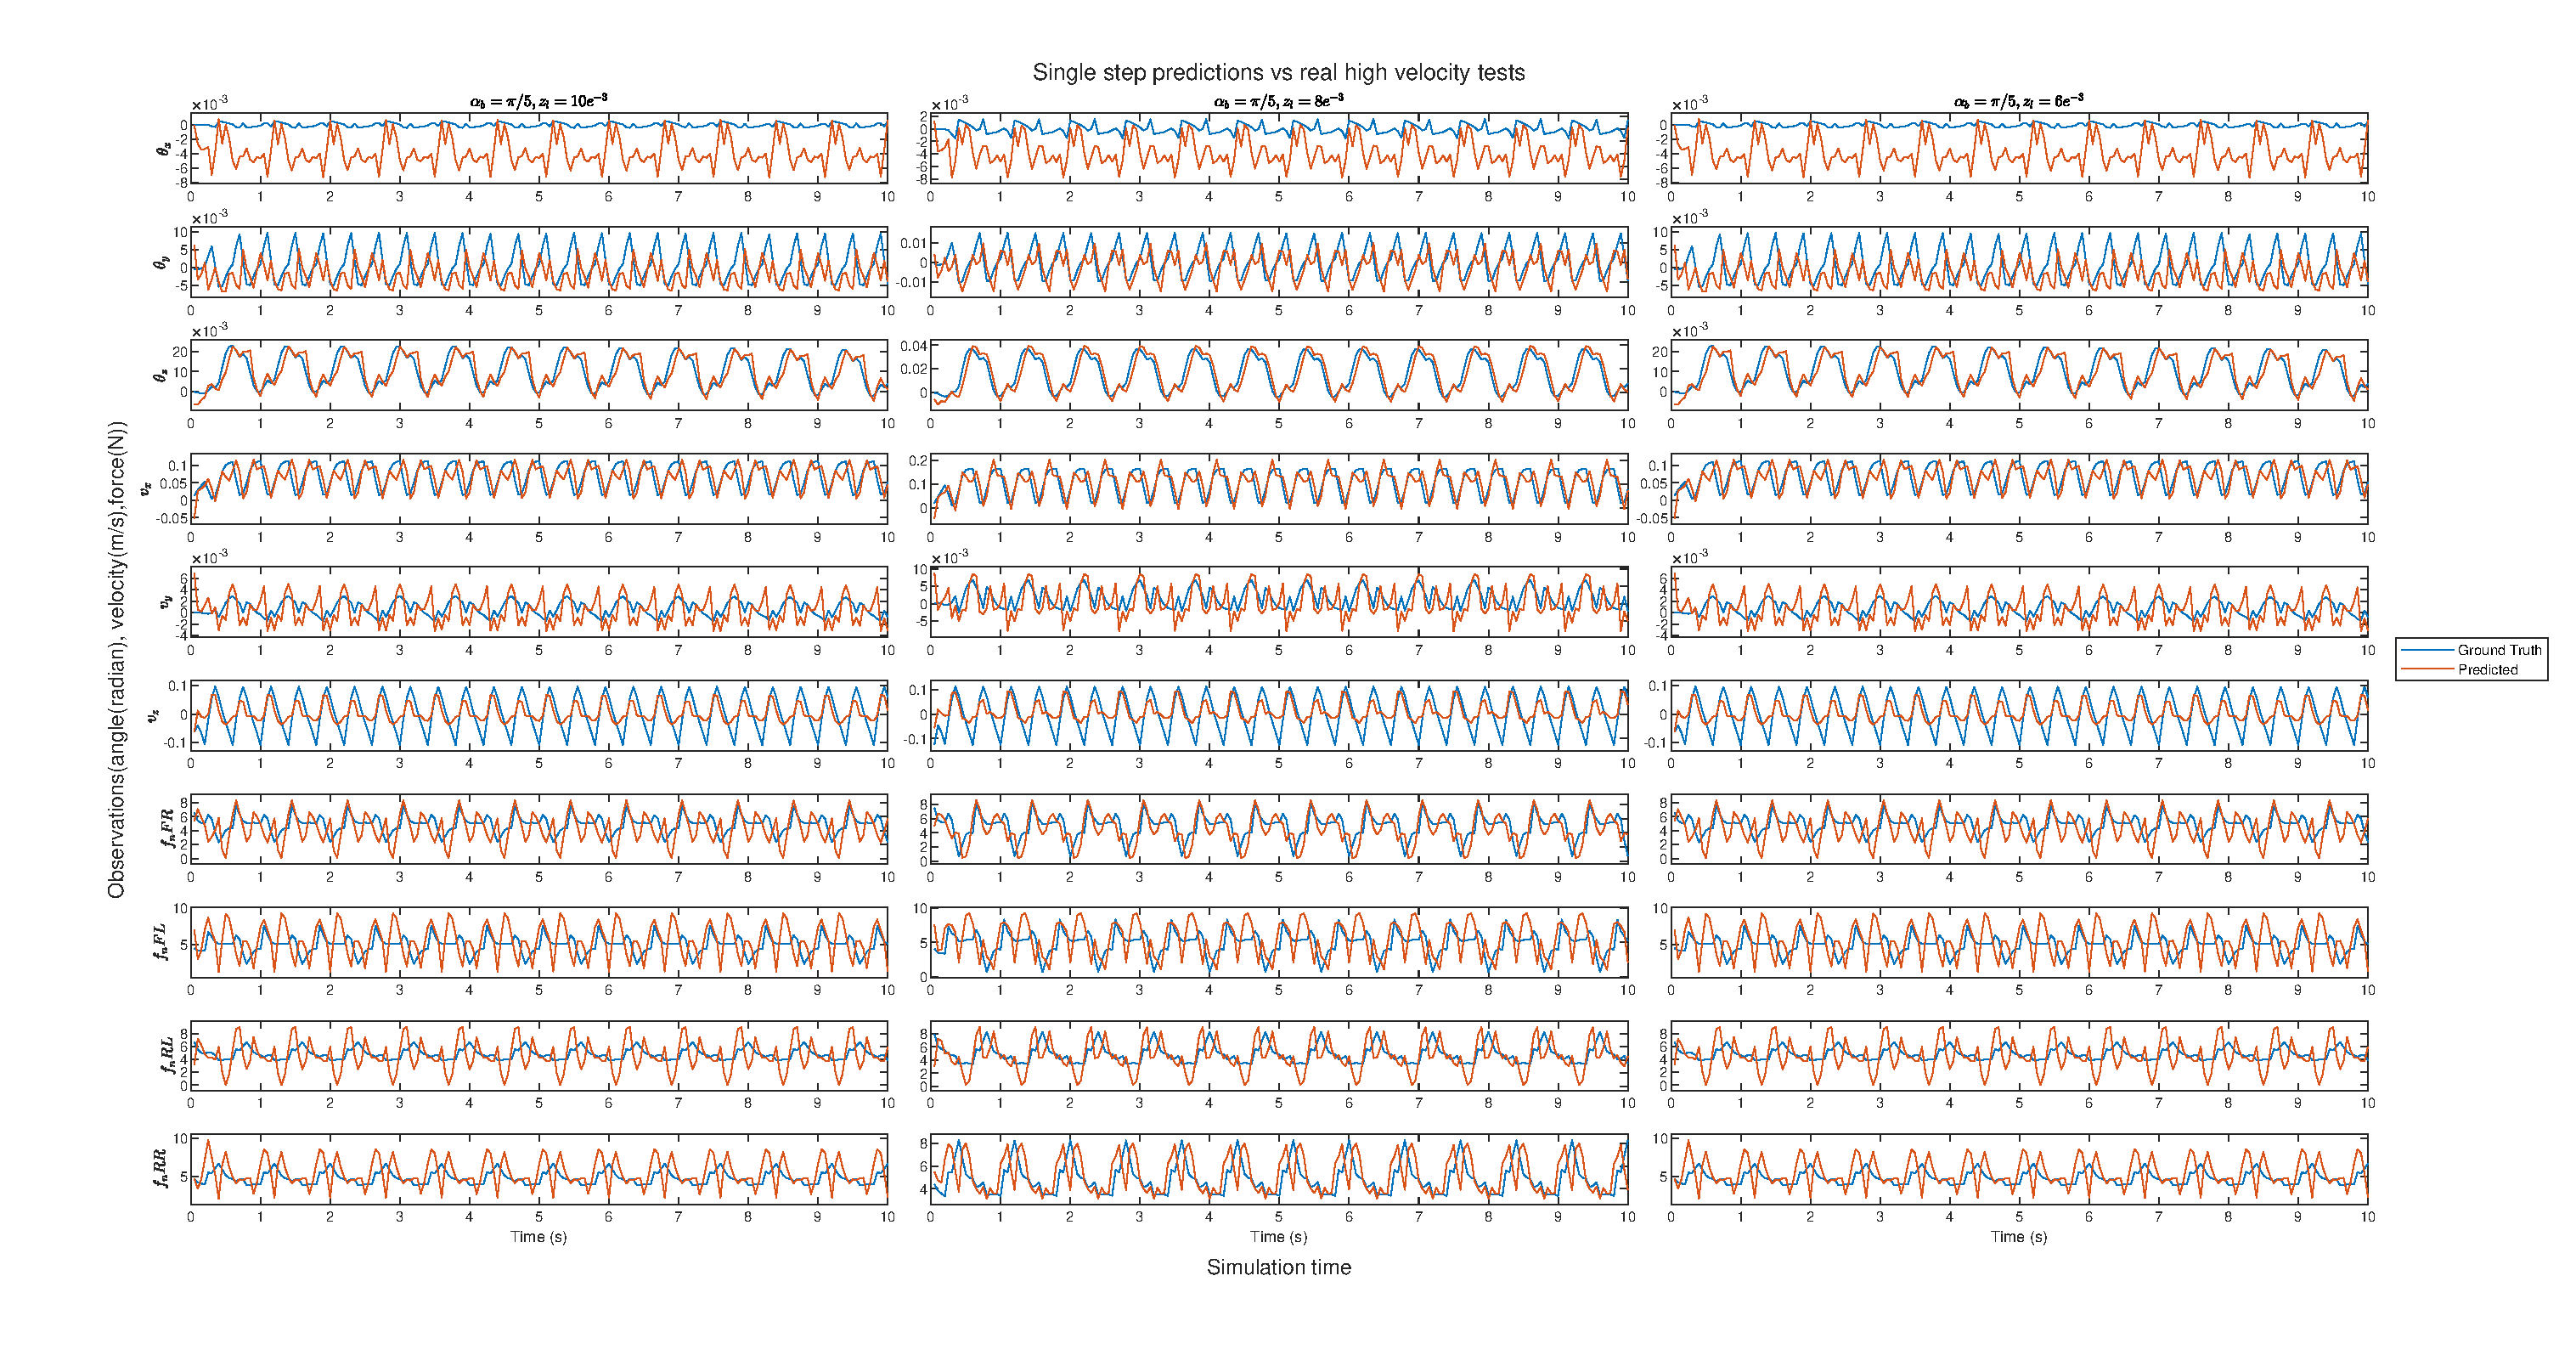
\includegraphics[width=\linewidth]{img/AppA/model_all.eps}
    \caption{Single step prediction test of DNN}
    \label{fig:DNN_test}
\end{figure}



\chapter{Source Code and Block Diagrams}
In this chapter, the main the source code and block diagrams implemented in Simulink is provided. These elements play a crucial role in this thesis, enabling the replication of experiments, validation of results, and the potential for further advancements in our work.


\section{Main Code of SoftQ}
github: 


\section{Block Diagrams from Simulink}
github: 


% 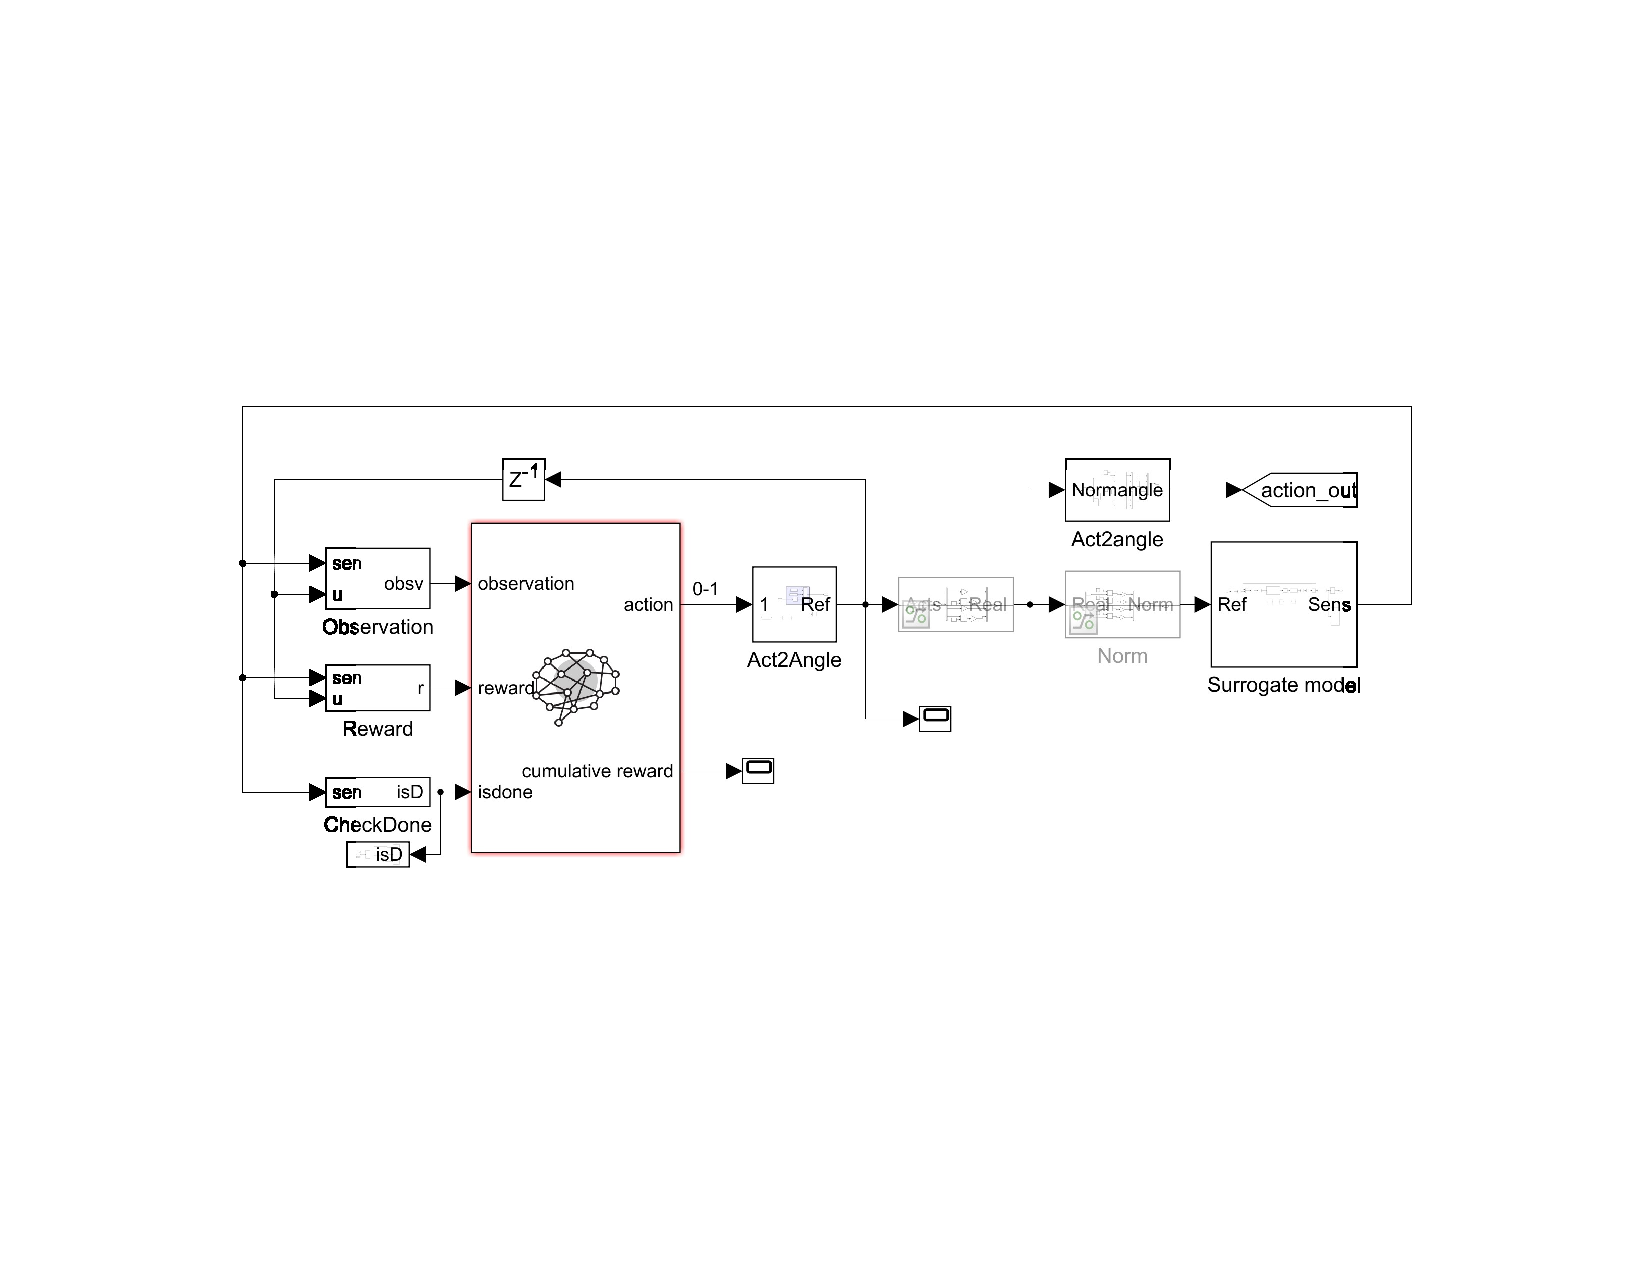
\includepdf[landscape=true]{img/AppB/it.pdf}
\subsection{Block Diagrams for Continue Training and MFRL}

\subsection{Block Diagrams for Simulink Controller}
\newpage
\newgeometry{top=56mm,bottom=30mm,left=26mm, right=35mm}
\definecolor{kth-blue}{RGB/cmyk}{25,84,166/0.849,0.494,0,0.349} 
\thispagestyle{empty}
% This is the last page of the document
% \begin{textblock*}{10cm}(38.83pt, {\paperheight - 70pt}) % {block width} (coords) 
% \noindent{\fontsize{10}{12} TRITA – ITM-EX 2023:XXX}
% \end{textblock*}

\begin{textblock*}{5cm}(38.83pt, {\paperheight - 44pt}) % {block width} (coords)  - was 44pt
\noindent{\fontsize{8}{9} 
    \textcolor{kth-blue}{\href{www.kth.se}{www.kth.se}}
}
\end{textblock*}
\begin{textblock*}{510pt}(38.83pt, {\paperheight - 34pt}) % {block width} (coords) - was 24.634pt
\begin{tikzpicture}
\draw[kth-blue, line width=1.0 pt] (0pt,0pt) -- (510pt,0pt);
\end{tikzpicture}
\end{textblock*}
% \thispagestyle{empty}
% \AddToShipoutPictureBG*{%]
%     \AtPageLowerLeft{%
%         
\includegraphics[width=1.0\paperwidth]{setup/img/kth-footer.png}
%     }%
% }

% \PlaceText{140mm}{272mm}{\color{white}\fontsize{10}{0} TRITA – ITM-EX 2023:XXX }


% \PlaceText{20mm}{282mm}{\color{white}\fontsize{12}{0}\sffamily \href{www.kth.se}{www.kth.se}}

%TC:endignore
\end{document}
